\documentclass[11pt,fleqn,a4paper,titlepage]{article} 
\addtolength{\textwidth}{1.5cm} 
\addtolength{\marginparwidth}{-20pt}
\usepackage{fancyhdr}
\usepackage{graphics}
\usepackage{graphicx}
\usepackage{geometry}
\usepackage[comma,authoryear]{natbib}
\usepackage[dvipsnames]{xcolor}
\pagestyle{fancy} 


% ======================================================
% i comandi seguenti impediscono la scrittura in maiuscolo 
% dei nomi dei capitoli e dei paragrafi nelle intestazioni 
\renewcommand{\sectionmark}[1]{\markboth{#1}{}} 
\renewcommand{\sectionmark}[1]{\markright{\thesection\ #1}} 
%\renewcommand{\subsectionmark}[1]{\markboth{#1}{}} 
%\renewcommand{\subsectionmark}[1]{\markright{\thesubsection\ #1}} 
\fancyhf{} % rimuove l�attuale contenuto dell�intestazione 
% e del pi\�e di pagina 
\fancyhead[LE,RO]{\bfseries\thepage} 
\fancyhead[LO]{\bfseries\rightmark} 
\fancyhead[RE]{\bfseries\leftmark} 
\renewcommand{\headrulewidth}{0.5pt} 
\renewcommand{\footrulewidth}{0pt} 
\addtolength{\headheight}{0.5pt} % riserva spazio per la linea 
\fancypagestyle{plain}{% 
\fancyhead{} % ignora, nello stile plain, le intestazioni 
\renewcommand{\headrulewidth}{0pt} % e la linea 
}
% ======================================================

\renewcommand{\familydefault}{\sfdefault}

\newcommand\selen{\textsf{SELEN~}}
\newcommand\selens{\textsf{SELEN}}
\newcommand\mmyr{mm~yr$^{-1}$}
\newcommand\ntg{$N_{tg}$~}
\newcommand\nv{$N_{v}$~}
\newcommand\sealevel{sea level~}
\newcommand\sealevels{sea level}
\newcommand\gmslr{GMSLR}
\newcommand\jgr{J. Geophys. Res.~}
\newcommand\gjras{Geophys. J. R. Astron. Soc.~}
\newcommand\gji{Geophys. J. Int.~}
\newcommand\grl{Geophys. Res. Lett.~}
\newcommand\eos{Eos. Trans. AGU~}
\hyphenation{SELEN}


\begin{document} 
\thispagestyle{empty}
\newgeometry{left=1.5cm,right=1.5cm,top=2cm,bottom=2cm}
\begin{figure}[!h]
\centering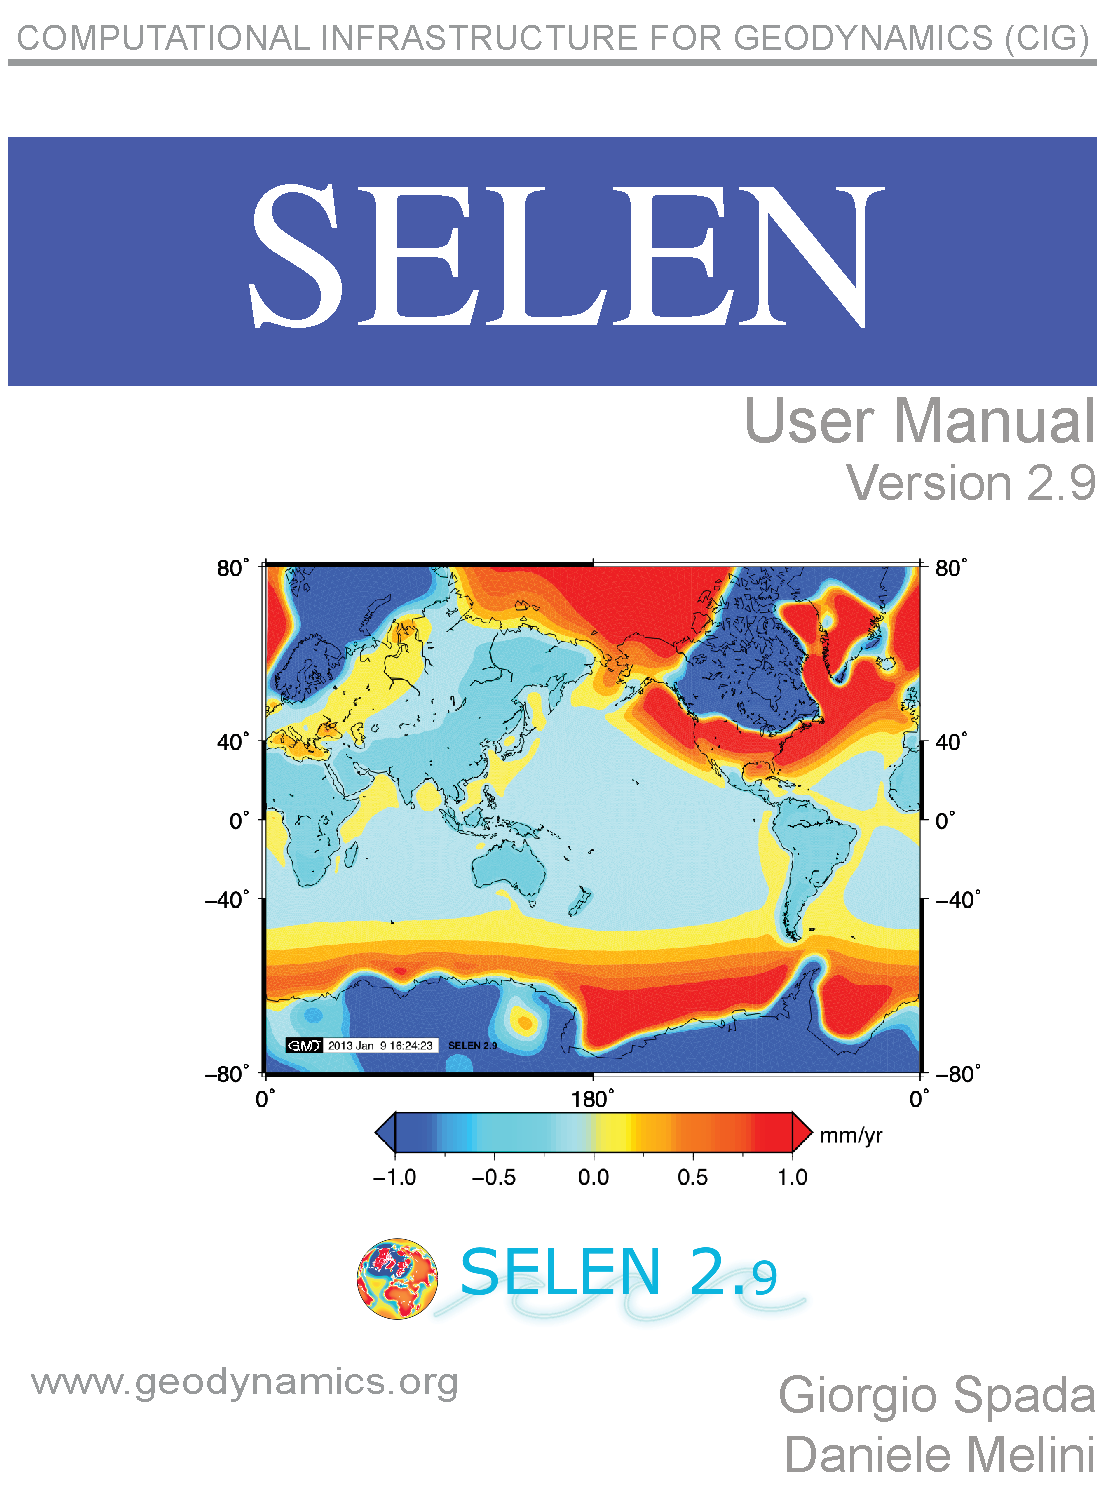
\includegraphics[width=\textwidth]{./Figures/selen-cover.pdf}
\end{figure}
\restoregeometry
\pagebreak

\title{{\underline {\large \textbf{COMPUTATIONAL INFRASTRUCTURE FOR GEODYNAMICS (CIG)}}}\\
\vspace{0.3cm}
\large{http://www.geodynamics.org/} \\
\vspace{1.1cm}
%
\includegraphics[angle=0,width=0.9\textwidth]{./Figures/logo_SELEN29.png}
\Huge{{SELEN: a program for solving the \\ \textit{``Sea Level Equation''}}} \\ 
\vspace{0.6cm}
\Large{User Manual for version 2.9} \\
\vspace{0.7cm}
\normalsize{Giorgio Spada (giorgio.spada@gmail.com)} \\
\normalsize{DiSBeF, Universit\`a di Urbino} \\
\vspace{0.55cm}
\normalsize{Daniele Melini (daniele.melini@ingv.it)} \\
\normalsize{Istituto Nazionale di Geofisica e Vulcanologia (INGV)} \\
\vspace{0.55cm}
%\normalsize{xy} \\
%\normalsize{abc} \\
%\vspace{0.15cm}
%\normalsize{xy} \\
%\normalsize{abc} \\
\vspace{0.7cm}
\texttt{\small{Manual version 1.2, November 2015}}\\
\vspace{0.9cm}

\includegraphics[angle=0,width=0.75\textwidth]{./Figures/logo_SELEN29.png}
\vspace{-0.5cm}
}
%\Huge logo here 
%\Huge logo here 
%\Huge logo here 


%\begin{figure}[h]
%\begin{center}
%
\includegraphics[angle=0,width=0.7\textwidth]{./Figures/logo_SELEN29.png}
%\label{fig:logo} 
%\end{center} 
%\end{figure}

%\vspace{0.2cm}
%\normalsize{Florence Colleoni (f.colleoni@gmail.com)} \\
%\normalsize{Centro Euromediterraneo per i Cambiamenti Climatici (CMCC)} \\

\maketitle

\newpage

\tableofcontents
\let\thefootnote\relax\footnotetext{The cover image is a GMT visualization of the rate of sea level change today (\textit{\sealevel fingerprint}) associated with GIA ($\dot S$) calculated by SELEN. Details about parameters and analysis are in Figure \ref{fig:sdot} in this manual.}

\listoffigures

\listoftables

\clearpage 

\begin{figure}[h]
\begin{center}
\vspace{6cm}

\includegraphics[angle=0,width=1\textwidth]{./Figures/logo_SELEN29.png}
\vspace{0cm}
\caption[The \selen logo]{\small{The \selen logo is an artwork by Florence Colleoni (2009).}}
\label{fig:logo} 
\end{center} 
\end{figure}

\clearpage 

\section{Introduction}\label{introduction}

The open source program \selen solves numerically the so--called ``Sea Level Equation'' (SLE) for a spherical, layered, non--rotating Earth with Maxwell viscoelastic rheology. 

The SLE  is an integral equation that was introduced in the $70$s to model the \sealevel variations in response to the melting of late--Pleistocene ice--sheets, but it can also be employed for predictions of geodetic quantities in response to present-day melting of continental ice-sheets. \selen can compute vertical and horizontal surface displacements, gravity variations and \sealevel changes on a global and regional scale. 

\selen (acronym of SEa Level EquatioN solver) is particularly oriented to scientists at their first approach to the glacial isostatic adjustment (GIA) problem and, according to our experience, it can be successfully used in teaching. The current release (2.9) considerably improves the previous version of the code in terms of computational efficiency, portability and versatility. As far as we know, 
\selen is the only open source program designed for solving the SLE. 

\selen 2.9 solves the SLE following the classical theory of \citet{Farrell_and_Clark_1976}. In the future release of \selen (\selen 3.0), which is under development, two important new features will be introduced: the rotational feedback on \sealevel and the horizontal migration of shorelines in response to \sealevel change. 

This User guide describes the essentials of the theory behind the SLE, and provides instructions for the configuration and execution of \selens. 

\section{Acknowledgements}
We thank all the \selen users and a number of colleagues for the numerous feedbacks that have greatly contributed to improve the program. We thank Max Tegmark for making available the code for the icosahedral pixelization of the sphere. For computations involving spherical harmonic functions, \selen implements some {SHTOOLS} routines developed by Mark Wieczorek. All the figures have been drawn using the free GMT software \citep{Wessel_and_Smith_1998}. The development of \selen has been supported by ISCRA (Italian SuperComputing Resource Allocation) with contracts n. HP10CS9J50 (SEASIM) and HP10CUX77T (SEAMED). Partly funded by COST Action ES0701 ``Improved Constraints on Models of Glacial Isostatic Adjustment'' and by the European Commission's 7$^{\textrm{th}}$ Framework Programme through grant number 226375 (ice2sea project). CIG is thanked for hosting SELEN (\texttt{http://geodynamics.org/cig/software/selen}). Eric Heien from CIG has greatly improved the \selen usability by implementing the autoconf system into the original code.

\section{Citation}
Computational Infrastructure for Geodynamics (CIG) and the SELEN developers are making the source code to SELEN available to researchers in the hope that it will aid their research and teaching.  A number of individuals have contributed a significant amount of time and energy into the development of SELEN.  We request that you cite the appropriate papers and make acknowledgements as necessary. The SELEN development team asks that you cite the following papers:

\begin{itemize}
\item Spada G, Stocchi P (2006) The Sea Level Equation, Theory and Numerical Examples. Aracne, Roma.
\item G. Spada, P. Stocchi, SELEN: A Fortran 90 program for solving the �sea-level equation�, Computers \& Geosciences, Volume 33, Issue 4, May 2007, Pages 538-562, ISSN 0098-3004, http://dx.doi.org/10.1016/j.cageo.2006.08.006 .
\item Spada G, Melini D, Galassi G, Colleoni F (2012) Modeling sea level changes and geodetic variations by glacial isostasy: the improved SELEN code (http://arxiv.org/abs/1212.5061)
\end{itemize}

\clearpage

\section{Theoretical background}\label{sec:theory}

Here we briefly illustrate the background theory of the SLE, the integral equation that describes the \sealevel variations and solid Earth deformations associated with GIA. Essentially, the material that follows is a condensed summary of the SLE theory first exposed by \citet{Farrell_and_Clark_1976}. 

For further details, including the spatiotemporal discretization of the SLE and its  numerical implementation, the reader is referred to the review of \citet{Spada_and_Stocchi_2006} and to references therein. 

\subsection{Sea Level and Sea Level change}\label{sec:slc}

Introducing the SLE requires some basic definition involving the general concept of ``\sealevels''. 
\emph{Absolute \sealevels} is:
\begin{equation}\label{eq:sl-def}
\textrm{SL}(\omega,t) = R_{ss}(\omega,t) - R_{se}(\omega,t), 
\end{equation}
where $\omega\equiv (\theta,\lambda)$, $\theta$ is colatitude and $\lambda$ is longitude, $t$ is time, and
$R_{ss}$ and $R_{se}$ denote the radii of the (equipotential) sea surface and of the solid surface 
of the Earth, both relative to the Earth's center of mass (CM). 

The quantity involved in the SLE is \emph{sea level change}
\begin{equation}\label{eq:s-definition}
S(\omega, t) = \textrm{SL}(\omega,t) - \textrm{SL}(\omega,t_{r}), 
\end{equation}
where $t_{r} \le t$ denotes a remote time. For studies 
of past \sealevel variations, it is convenient to introduce 
\emph{relative sea level} (RSL):
\begin{equation}
\textrm{RSL}(\omega,t_{BP})=\textrm{SL}(\omega,t_{BP})- \textrm{SL}(\omega,t_{p}),
\end{equation}
where $t=t_{BP}$ is a given time before present (BP) and $t=t_p$ is present time. 
Using (\ref{eq:s-definition}), {RSL} is easily expressed in terms of \sealevel change: 
\begin{equation}\label{eq:rsl-vs-s}
\textrm{RSL}(\omega,t_{BP})= {S}(\omega,t_{BP})- {S}(\omega,t_{p}).
\end{equation}

An expression for $S(\omega, t)$ which is suitable in GIA studies is 
obtained using (\ref{eq:sl-def}) in
(\ref{eq:s-definition}): 
\begin{equation}\label{sle-original}
S(\omega, t) = N(\omega,t) - U(\omega,t), 
\end{equation}
where $N(\omega,t)= R_{ss}(\omega,t) - R_{ss}(\omega,t_r)$ is the \textit{sea surface variation} relative to the CM (sometimes referred to as \emph{absolute \sealevel change}) and $U(\omega,t)= R_{se}(\omega,t) - R_{se}(\omega,t_r)$ is the \emph{vertical displacement} of the solid surface of the Earth. Note that $S(\omega, t)$ is defined over the whole Earth surface, including the continental masses. 

Eq.~(\ref{sle-original}) represents the SLE in its simplest form; 
what follows is aimed to illustrate the relationship between $S$ and the variations of the ice thickness through time, in order to obtain a form of the SLE amenable to a numerical approach. 

\subsection{The Sea Level Equation}\label{sec:sle}

According to \citet{Farrell_and_Clark_1976}, the sea surface variation $N$ in Eq.~(\ref{sle-original}) can be written as 
\begin{equation}\label{n_sle}
{N}(\omega, t) = G(\omega, t) + c(t),  
\end{equation}
where $c$ is yet undetermined and the \emph{geoid height variation} is 
\begin{equation}\label{g_sle}
G(\omega, t) = \frac{\Phi}{\gamma}(\omega, t),  
\end{equation}
in which $\gamma$ is the reference gravity at the surface of the Earth and $\Phi(\omega,t)$ is the 
\emph{total
variation of the gravity potential}. 

Hence, using Eq.~(\ref{n_sle}) into (\ref{sle-original}) gives 
\begin{equation}\label{sle-c}
S(\omega, t) = \frac{\Phi}{\gamma} - U +c, 
\end{equation}
where we have dropped the ($\omega,t$) dependence in right hand side to simplify notation. Mass
conservation of the system (Ice sheets + Oceans) is ensured taking   
\begin{equation}\label{c-constant}
c(t) = - \frac{m_i}{\rho_{w}A_{o}} - \overline{ \biggl( \frac{\Phi}{\gamma} - U\biggr)}, 
\end{equation}
where $\rho_{w}$ is the (constant) density of water, $m_{i}$ is the mass 
variation of the ice sheets, $A_{o}$ is the (constant) area of the present--day oceans 
and the overbar indicates the average over the surface of the oceans 
\begin{equation}\label{average}
\overline {(\ldots)} = \frac{1}{A_{o}} \int_{o} (\ldots) ~dA,
\end{equation}
where $dA=a^{2}\sin\theta d\theta d\lambda$ is the area element 
and $a$ is Earth average radius. From Eq.~(\ref{sle-c}), the SLE can be therefore written as 
\begin{equation}\label{slegia}
S(\omega,t) = \biggl( \frac{\Phi}{\gamma} - U\biggr)  +S^E   - \overline{ \biggl( \frac{\Phi}{\gamma} - U\biggr)}, 
\end{equation}
where the \emph{``eustatic'' \sealevel variation}: 
\begin{equation}\label{eustatic}
S^{E}(t) = - \frac{m_i}{\rho_w A_o},  
\end{equation}
shows the remarkable property 
\begin{equation}
S^{E}(t) = \overline{S}. 
\end{equation}
\noindent The SLE has solution $S=S^{E}$ only in the case of a rigid, 
non self--gravitating Earth ($U = \Phi = 0$ in Eq.~\ref{slegia}).

Functions $U(\omega,t)$ and $\Phi(\omega,t)$ will depend on the spatiotemporal variations of the 
\emph{surface load}:  
\begin{equation}\label{load}
{\cal L}(\omega,t) = \rho_{i}I + \rho_{w} S {\cal O},
\end{equation}
where the two terms on the right hand side are associated with the waxing and waning of the ice sheets 
(\textit{ice load}), and with the redistribution of meltwater in the ocean basins (\textit{ocean load}), 
respectively. 
In Eq.~(\ref{load}), $\rho_i$ is ice density, ${\cal O}$ is the \emph{ocean function}   
\begin{equation}\label{eq:ocean-function}
{\cal O}(\omega) = \left\{ \begin{array}{ll} 
1, & \textrm{if~} \omega \in \textsf{oceans}\\ 
0, & \textrm{if~} \omega \in \textsf{land,} 
\end{array} \right. 
\end{equation} 
(hereinafter referred to as OF), and   
\begin{equation}\label{ice-thick-variation}
I(\omega,t)= T - T_0, 
\end{equation}
is the \emph{ice thickness variation}, where $T(\omega,t)$ is \emph{ice thickness}, and $T_{0}(\omega)$ is a reference 
thickness at a remote time ({e.g.} the thickness at the Last Glacial Maximum, LGM, $21$ kyrs ago). The mass variation in 
Eq.~(\ref{eustatic}) is obtained from (\ref{ice-thick-variation}) by integration over the 
ice--covered regions: 
\begin{equation}\label{mass-variation}
m_{i} (t)= \int_{i} \rho_{i}I ~dA.  
\end{equation}
Following Eq.~(\ref{load}), vertical displacement stems from two terms
\begin{equation}\label{u_sle}
{U}(\omega, t) = \rho_i G_{u}\otimes_i I + \rho_w G_{u}\otimes_o S,  
\end{equation}
where $G_{u}$ is the {Green's} function for vertical displacement, 
$\otimes_i$ and $\otimes_o$ are spatiotemporal convolutions 
over the ice-- and ocean--covered regions, respectively (these convolutions and the Green's functions 
are formally defined in \citeauthor{Spada_and_Stocchi_2006}~\citeyear{Spada_and_Stocchi_2006}). Similarly, the total
variation of the gravity potential is
\begin{equation}\label{phi_sle}
\Phi(\omega,t) = \rho_i G_{\phi}\otimes_i I + \rho_w G_{\phi}\otimes_o S,  
\end{equation}
where $G_{\phi}$ is the corresponding {Green's} function. Explicit expressions for $G_u$ and $G_{\phi}$ are given in e.g.~\citet{Spada_and_Stocchi_2006} in terms of the load--deformation coefficients (LDCs) $h(t)$ and $k(t)$, respectively. The \sealevel Green's function is defined as the difference:  
\begin{equation}\label{gf_sl}
\frac{G_{s}}{\gamma}(\omega,t) =    \frac{G_{\phi}}{\gamma} - {G_{u}}. 
\end{equation}

Substitution of Eqs. (\ref{u_sle}) and (\ref{phi_sle}) into (\ref{slegia}) using (\ref{gf_sl}) gives 
\begin{equation}\label{sle}
S(\omega, t) = \frac{\rho_i}{\gamma} G_s^{} {\otimes}_i I + \frac{\rho_w}{\gamma} G_s^{} {\otimes}_o S 
                             + S^E 
-\frac{\rho_i}{\gamma} \overline {G_s^{} {\otimes}_i I}
-\frac{\rho_w}{\gamma} \overline {G_s^{} {\otimes}_o S}, 
\end{equation}
which represents the SLE in the \emph{``gravitationally self--consistent''} form. Since the unknown $S(\omega,t)$ also appears in the spatiotemporal convolutions at the right hand side, the SLE is an integral equation, which in general cannot be solved in closed form. 
The SLE is a linear equation as long as shorelines are not allowed to migrate horizontally, i.e. if ${\cal O}$ (and consequently $A_o$) 
is not dependent on $S$ itself. Sea level variations are sensitive to mantle rheology through $G_{s}$, since this is determined by the viscoelastic LDCs $h$ and $k$ \citep{Spada-2003a, Spada_and_Stocchi_2006}. Solutions of Eq.~(\ref{sle}) in special cases, discussed in detail by \citet{Spada_and_Stocchi_2006}, are also available via \selen. 

It is worth to observe that the SLE (\ref{sle}) does not involve absolute quantities and can, consequently, only provide \textit{variations} of geophysical and geodetic quantities relative to a reference state. 

\subsection{Solving the Sea Level Equation}\label{sec:solve-the-sle}

The form (\ref{sle}) of the SLE is not suitable for a numerical implementation. In fact,
the spherical harmonic (SH) decomposition of terms terms like $ G_s^{}{\otimes}_o S$, which 
imply an integration over the oceans and not over the whole Earth, would demand evaluating 
coupling coefficients between sets of SHs, which may severely limit the maximum degree of the 
harmonic analysis (SH conventions in \selen are summarized in Section~\ref{sec:shs}). 

The \emph{pseudo--spectral approach} introduced {by \citet{Mitrovica_and_Peltier_1991} 
and}  \citet{Mitrovica_etal_1994}, and implemented in \selens, overcomes this difficulty, since 
it allows for a direct spectral analysis \citep{Milne_1998}. {At the core of the 
method is a change of variable in the SLE, where $S(\omega,t)$ is substituted by its projection on the OF:
\begin{equation}
Z(\omega,t) \equiv {\cal O}S,
\end{equation}
where we define $Z$ as the \emph{modified \sealevel change}. Multiplying both sides of 
Eq.~(\ref{sle}) by ${\cal O}$ gives the SLE in the form:
\begin{equation}\label{eq:sle-z}
Z(\omega,t) = H  + Z^E + K(Z), 
\end{equation}
where: 
\begin{eqnarray}
Z^E(t)      & \equiv & {\cal O}S^E \\
H(\omega,t) & \equiv &{\cal O}(A - \overline{A}) \\
K(Z;\omega,t) & \equiv & {\cal O}(B - \overline{B}), 
\end{eqnarray}
and variables 
\begin{eqnarray}
A(\omega,t) &\equiv & \frac{\rho_i}{\gamma}~ G_s {\otimes}_e I \label{eq:adef}\\
B(\omega,t) &\equiv & \frac{\rho_w}{\gamma}  G_s {\otimes}_e Z \label{eq:bdef},
\end{eqnarray}
now involve an integration (denoted by ${\otimes}_e$) over the whole Earth's surface, which can
be tackled using a standard spectral approach. Using this formalism, the SLE (\ref{sle}) reads 
\begin{equation}\label{eq:sle-ab}
S(\omega,t) = A - \overline{A} + S^E + B - \overline{B}  
\end{equation}
and from (\ref{u_sle}) vertical displacement is  
\begin{equation}\label{u-ab}
U(\omega,t) = A_u + B_u,
\end{equation}
where $A_u$ and $B_u$ have the same form of $A$ and $B$ in (\ref{eq:adef}) and (\ref{eq:bdef}), but with $G_s$ replaced by $G_u$. 
Similarly, from (\ref{phi_sle}) and (\ref{g_sle}), the geoid height variation is  
\begin{equation}\label{g-ab}
G(\omega,t) = A_g + B_g,
\end{equation}
where $A_g$ and $B_g$ have the same form of $A$ and $B$, with $G_s$ replaced by $G_\phi$.

Since term $K$ in (\ref{eq:sle-z}) depends on $Z$, the SLE is an integral (implicit) equation, in which the unknown $Z$ appears explicitly at the left--hand side but it is convolved in space and time with $G_s$ on the right hand side. This suggests an iterative approach to the SLE, similar to that employed to solve the one--dimensional inhomogeneous integral Fredholm equations of the second kind. However, the complexity of the SLE (and its three dimensionality) hinders an analytical study of the convergence conditions of the iteration scheme. 

Following \citet{Spada_and_Stocchi_2007}, to which the author is referred for 
more details, the iteration scheme implemented in \selen reads 
\begin{equation}\label{eq:iteration-scheme}
\left\{ \begin{array}{ll} 
Z^{(0)}_{\ell m,i} = & Z^E_{\ell m,i} \\
Z^{(k)}_{\ell m,i} = & H_{\ell m,i}  + Z^E_{\ell m,i} + K_{\ell m,i}\left(Z^{(k-1)}_{\ell'm',j}\right),  
\end{array} \right. 
\end{equation} 
where $Z^{(k)}_{\ell m,i}$ is the $k$--th approximation to the degree $\ell$ ($0 \le \ell \le \ell_{max}$) and order $m$ ($0 \le m \le \ell$) component 
of $Z(\omega,t)$, evaluated at the $i$--th time step (a piecewise constant behavior is assumed for all the 
variables involved in the SLE, with a typical time step of $1$ kilo--year). The iteration continues until the ratio 
$|Z^{(k)}_{\ell m,i}-Z^{(k-1)}_{\ell m,i}|$/$|Z^{(k-1)}_{\ell m,i}|$  becomes sufficiently small (according to the numerical tests carried out by \cite{Spada_and_Stocchi_2007}, three to five iterations normally suffice for convergence). Once the SLE is solved, all the other geophysical and geodetic quantities (see e.g. \citeauthor{Spada_etal_2012a}~\citeyear{Spada_etal_2012a}) 
are immediately obtained from the spectral components of Eqs.~(\ref{eq:sle-ab}), (\ref{u-ab}), and (\ref{g-ab}). 

For the numerical evaluation of surface integrals embedded in terms $H$ and $K$ of the SLE 
(Eq.~\ref{eq:sle-z}), \selen takes advantage of the equal--area, icosahedron--shaped, spherical 
pixelization by \citet{Tegmark_1996}, which is particularly convenient for the manipulation 
of harmonic functions.  
The number of pixels on the grid is determined by 
\begin{equation}\label{eq:np}
N_p = 40R(R+1) + 12, 
\end{equation} 
where the integer $R$ is the \textit{grid resolution parameter} \citep{Tegmark_1996}. The pixels 
are the centers of slightly distorted hexagonal grid cells. Assuming that $N_p$ is sufficiently large, 
the area of the surface of the cells is $A_{cell}\sim 4\pi a^2/N_p$
and their radius is $r_{cell} \sim a\sqrt{4/N_p}$, where $a$ is Earth's radius. 
As discussed by \citet{Tegmark_1996}, an accurate numerical integration of harmonic functions up 
to degree $\ell_{max}$ demands a sufficiently large number of grid pixels, with  
\begin{equation}\label{eq:constraint-lmax-r}
N_p \ge \frac{\ell^2_{max}}{3}, 
\end{equation}
where $\ell_{max}$ is the maximum harmonic degree of the SH expansion of the SLE. 

\clearpage

\section{How \selen works}\label{sec:how}

\subsection{Software and hardware requirements}\label{sec:sw-hw}

\paragraph{Software.} Running \selen requires a standard UNIX environment (including Linux and Mac OS X) and a Fortran 90 compiler. On Windows systems, \selen can run within the Cygwin environment\footnote{Cygwin is freely downloadable from: http://www.cygwin.com}. \selen also requires the free GMT\footnote{The Generic Mapping Tools can be downloaded from: http://gmt.soest.hawaii.edu/} (Generic Mapping Tools) mapping software \citep{Wessel_and_Smith_1998}.  

The configuration and build process of \selen 2.9 is handled by standard GNU autoconf scripts\footnote{http://www.gnu.org/software/autoconf/}.  \selen 2.9 has been succesfully tested using both the freely available g95\footnote{Available from: http://www.g95.org} and gfortran\footnote{Available from: http://gcc.gnu.org/gfortran} compilers, or the commercial Intel Fortran compiler\footnote{More information at: http://software.intel.com/en-us/fortran-compilers}. Additional operating system and compiler configurations can be implemented by modifying the \texttt{flags.guess} file and providing suitable options to the \texttt{configure} script. 
%A list of currently supported operating systems and Fortran compilers is given in %\marginpar{T\ref{table:compiler-options}} Table~\ref{table:compiler-options}. 
%To run \selens, the GMT\footnote{The Generic Mapping Tools can be downloaded from: http://gmt.soest.hawaii.edu/} (Generic Mapping Tools) public domain software of \citet{Wessel_and_Smith_1998} must be installed on the system.  

%
%\begin{table}[!hbp]
%\begin{center}
%\caption[{Supported platforms}]{\selen supported operating system/compiler combinations. The code in the first column can be set by option \texttt{121} in \texttt{config.dat}.}
%\begin{tabular}{cl}
%\\
%\hline
%Code &  Description  \\
%\hline
%\texttt{1} & GNU gfortran on x86 Mac OS X\\
%\texttt{2} & Intel Fortran compiler on x86 Mac OS X\\
%\texttt{3} & GNU gfortran on x86 Linux\\
%\texttt{4} & Intel Fortran compiler on x86 Linux\\
%\texttt{5} & Reserved for future use\\
%\texttt{6} & IBM XL Fortran compiler on AIX\\
%\texttt{7} & GNU gfortran on Win32 CYGWIN environment\\
%\texttt{8} & G95 compiler on any system \\
%           & (suitable for Mac OS X on PowerPC)\\
%\hline
%\label{table:compiler-options}
%\end{tabular}
%\end{center}
%\end{table}
%

\begin{figure}[t]
\begin{center}
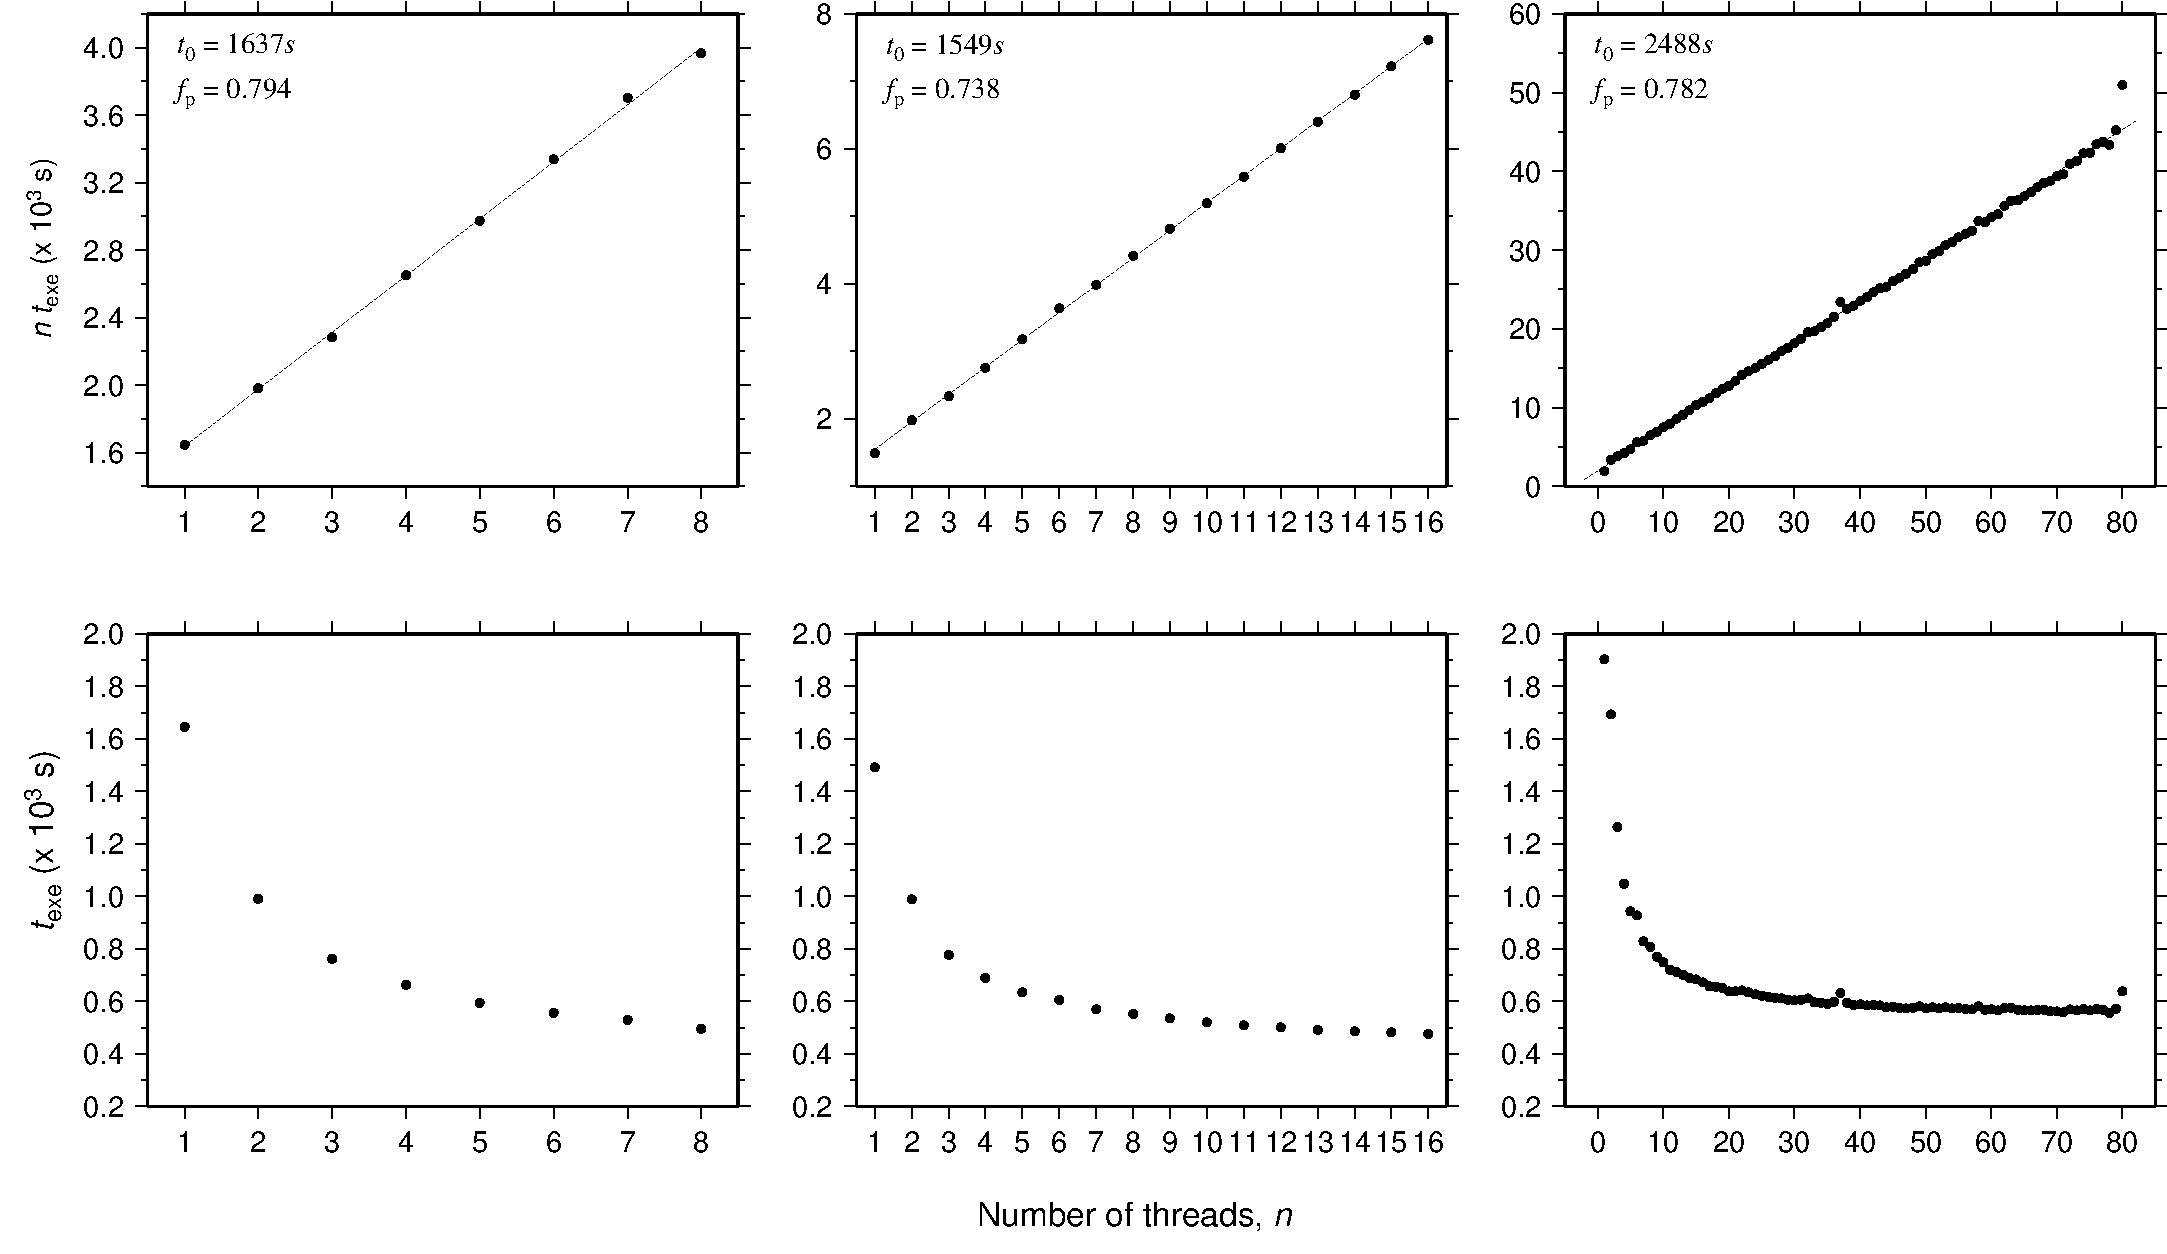
\includegraphics[width=0.9\textwidth,angle=0]{./Figures/scaling-new.pdf}
\caption[Execution time scaling]{\small{Scaling of execution time for the \texttt{TEST} run with the number of threads. Test systems are: an Apple Mac Pro configured with two 2.8GHz quad-core Intel Xeon CPUs (``Harpertown''--class, model number E5462) and 16GB DDR2 RAM, running Mac OS X 10.5.8 (left frames); an HP ProLiant BL460c G8 configured with two 2.70GHz eight-core Intel Xeon CPUs (``Sandy Bridge''--class, model number E5-2680) and 128GB DDR3 RAM, running Red Hat Enterprise Linux 5.8 (middle frames); 
an HP ProLiant DL98G7 configured with eight 2.0GHz 10-core Intel Xeon CPUs (``Westmere''--class, model number E7-2850) and 2TB DDR3 RAM, running Scientific Linux release 6.3 (right frames).  In top frames, a dashed line represent the fit of Eq.~(\ref{eq:amdahl2}) to the measured points; corresponding values of $t_0$ and $f_p$ are given for each system.}}
\label{fig:scaling}
\end{center}
\end{figure}

In \selen 2.9, the most computationally intensive portions of code have been parallelized with~\cite{Openmp_2005} directives. The corresponding program units can therefore take advantage of multi--threading on modern CPUs, resulting in a substantial performance improvement\footnote{The g95 compiler does not support OpenMP, so it is not possible to run \selen in parallel with this compiler.}. 

Porting \selen on ``unsupported'' systems should be an easy task.  The only tricky aspect is that program unit \texttt{tb.F90} (the LDCs calculator)  needs quad--precision floating--point (i.e. \texttt{REAL*16}), which is not supported on all platforms.  The Intel fortran compiler and the g95 compiler fully support \texttt{REAL*16} objects. On x86 systems, the GNU gfortran compiler does {not} support \texttt{REAL*16}; however it supports \texttt{REAL*10}, essentially a double-precision fraction with a quad--precision exponent, which is adequate for floating-point computations in \texttt{tb.F90}.  When porting \selen to other platforms, the support and range of \texttt{REAL*16} variables have to be carefully checked.

%A special attention should be paid to the \texttt{PATH} ~system ~variable ~when ~running \selen ~under the Cygwin environment. Since on Windows systems all executables have the \texttt{.exe} suffix, the \texttt{sh} shell binary has the same name of the executable for the \texttt{sh.f90} \selen program unit. To avoid confusion, if the current working directory (``\texttt{.}'') is included in the search path, it must be placed \textit{after} \texttt{/usr/bin}; for instance, with the command \texttt{PATH=\$PATH:.}.  In this way, it is guaranteed that the command (`\texttt{sh}') will invoke the \texttt{sh} shell and not the executable of the \texttt{sh.f90} \selen program unit. 

\paragraph{Hardware.} The hardware requirements of \selen are related to the desired grid resolution parameter $R$ and to the maximum harmonic degree $\ell_{max}$. For low or medium resolutions (approximately $R \le 50$ and $\ell_{max} \le 128$), \selen can run without trouble on a notebook.  High-resolution runs might require a multi-processor system and/or large amounts of RAM.   
The \texttt{TEST} \selen run, described in Section~\ref{section:test-run}, runs in about $34.5$ minutes on an Apple MacBook with a 2GHz dual-core Intel Core 2 Duo CPU and in about $10.5$ minutes on an Apple Mac Pro with two 2.8Ghz quad-core Intel Xeon CPUs.

The execution time of \selen scales with the number of grid pixels $N_p$ and the maximum harmonic degree $\ell_{max}$ as $t_{exe} \sim N_p N_h$ where
$N_h = {(\ell_{max}+1) (\ell_{max}+2)}/{2}$ is the number of SHs for $\ell\le \ell_{max}$. In view of Eq.~(\ref{eq:np}), as a rough approximation
\begin{equation}
t_{exe} \sim \left(R \ell_{max}\right)^2, 
\end{equation} 
where $R$ is the grid resolution parameter. The memory footprint of \selen follows a similar scaling law. For high resolution runs (large values of $\ell_{max}$ and consequently of $R$, see Eq.~\ref{eq:constraint-lmax-r}), disk I/O can become a considerable fraction of $t_{exe}$, and these relations may no longer be valid. 

On multi--core systems, \selen can use multi--threading to reduce computation time (multi--threading was not implemented in previous version of \selens). Multi--threading will automatically be enabled if it is supported by the system and, as a default, all the available cores are used. If the user wishes to leave some resources free for other tasks, the \texttt{OMP\_NUM\_THREADS} environment variable has to be set to the number of usable cores before launching \selen.

Fig.~\ref{fig:scaling} 
%\marginpar{F\ref{fig:scaling}} 
shows the execution time $t_{exe}$ of the \texttt{TEST} as a function of the number of threads $n$ for three test systems.  If the inter-process communication overhead is negligible, the relationship between $t_{exe}$ and $n$ is well approximated by
\begin{equation}\label{eq:amdahl1}
t_{exe}(n) = t_0 \left( f_s + \frac{f_p}{n} \right), 
\end{equation}
where $f_s$ and $f_p$ are the serial and parallel fractions of the code ($f_s+f_p=1$), and $t_0$ is the serial execution time \citep{Amdahl_1967}.  Eq.~(\ref{eq:amdahl1}) can be rewritten as
\begin{equation}\label{eq:amdahl2}
n t_{exe}(n) = t_0 \left( f_p + f_s n \right), 
\end{equation}
showing that when the speedup of the parallel portion of the code is linear, the relation between $nt_{exe}$ and $n$ is also linear. Measured values of $nt_{exe}$ for the \texttt{TEST} run are shown in Fig.~\ref{fig:scaling}. By fitting Eq.~(\ref{eq:amdahl2}) to the points in Fig.~\ref{fig:scaling} it is possible to evaluate the parallel fraction $f_p$ of the code, which for the \texttt{TEST} run is within $0.7$ and $0.8$. This value depends on the specific options selected in the \texttt{config.dat}; for instance, enabling the execution of the GMT scripts (which are sequential tasks) results in a lower parallelism level.


% ----------------------------------------------------------------------


\subsection{Configuration and execution files}
The configuration and the execution of the program involve several files and scripts 
in the \selen directory. For a normal execution of \selens,
the user only needs to edit and modify the configuration file {\texttt{config.dat}}. 

\vspace{0.3cm}
\noindent The relevant scripts and programs for configuration and execution are: 

\begin{description}
\item [\texttt{config.dat}] is the configuration file of \selens. It is a plain text file that can 
be easily configured by the user according to the specific tasks to be accomplished. The structure of the file and the configuration rules are described in detail in Section~\ref{sec:configuration} below. A sample {\texttt{config.dat}}, configured for a \texttt{TEST} run, is provided in Section~\ref{sec:sample-config}, 
%\item [\texttt{makeselen.sh}] is the execution shell script of \selens. It performs the 
%following tasks: \textit{i)} parsing of {\texttt{config.dat}} to identify the Fortran compilation 
%options \textit{ii)} compilation of SHTOOLS programs, \textit{iii)} compilation and execution of the setup program \texttt{config.f90} and \textit{iv)}
%execution of the shell script \texttt{selen.sh}. Script \texttt{makeselen.sh} also handles some 
%error conditions,
\item [{\texttt{config.f90}}] is the \selen setup program. This program \textit{i)} 
parses {\texttt{config.dat}}, \textit{ii)} creates the shell script  \texttt{selen.sh} which physically executes the \selen run, 
\textit{iii)} creates  the ``include file'' \texttt{data.inc}, which contains declarations useful to all the Fortran units needed
for the execution (the full list is given in 
\marginpar{T\ref{table:fortran-units}} 
Table~\ref{table:fortran-units}), \textit{iv)} creates the GMT scripts needed for visualization of the results. The implementation of new features in \selen will demand, in general, adding new subprograms to {\texttt{config.f90}} or modifying the existing ones.   The setup program also performs several checks on the input parameters, and exits with an error message if inconsistencies are found. 
\item [\texttt{selen.sh}] is a shell script, created by {\texttt{config.f90}}, containing execution commands for the Fortran units of \selen which are required to fulfill the user's tasks. 
This script also creates the \texttt{depot} directory structure where
the \selen outputs are stored, and purges the working directory from temporary files before and after the execution of the program.
\end{description}

\subsection{Input and output data}\label{sec:input-output}
\paragraph{Input.} The \selen input data are organized in several sub--directories:  
\begin{enumerate}
\item Folder {\texttt{DATA}} collects various files with information about geophysical and geodetic sites of interest and other miscellanea data, 
\item Folder {\texttt{ICE-MODELS}} contains the files describing the time chronology of each the ice models available by \selens,
\item Folder {\texttt{VSC}} stores a collection of viscosity profiles. 
\item Folder {\texttt{INPUTS}} stores user--generated input files, such as pixel table files, pre--computed SH coefficients at the grid pixels and SH coefficients of the ice thickness data. 
\end{enumerate}

\paragraph{Output.} 
The \selen outputs consist of:
\begin{enumerate}
\item ASCII files with various formats, 
\item PostScript and PDF graphic files, 
\item GMT scripts.
\end{enumerate}
\noindent After each run, \selen outputs are stored in a subfolder \texttt{depot-}\textit{name}, where \textit{name} is a 4--character label defined by the user in the \texttt{config.dat} file (see Section~\ref{sec:configuration}). The \texttt{depot} output subfolders are created into the \texttt{DEPOTS} folder of the \selen directory, and their structure is described in 
%\marginpar{T\ref{table:folders}} 
Table~\ref{table:folders}. 

Some of the \selen intermediate outputs, such as SH coefficients at the grid pixels, SH coefficients of the ice thickness data or pixel table files, can be reused as input files for subsequent \selen runs.  After a \selen run, these files are stored in the \texttt{run} folder of the \selen working directory; in order to make them available for later reuse, they have to be manually moved into the \texttt{INPUTS} folder.

\clearpage

\section{Setting up and running \selen}

\subsection{Installation}\label{sec:installation}
The installation of \selen is straightforward. The user just needs ~to ~un--zip ~the ~\selen ~package 
in any chosen folder.  If not already available on the system, a supported Fortran compiler and the GMT mapping software \citep{Wessel_and_Smith_1998} must be also installed.

\subsection{Configuration}\label{sec:configuration}
The configuration file of \selen is the plain text file \texttt{config.dat}. Here we describe its structure and illustrate the options available to the user. A sample configuration file, employed for a \texttt{TEST} run in Section~\ref{section:test-run}}, is listed 
in Section~\ref{sec:sample-config}. 

\vspace{0.6cm}
\noindent File \texttt{config.dat} is composed of two sections:

\begin{itemize}
\item  \texttt{SECTION 1}
contains the general settings of \selens. It defines the approximation (mode of solution) employed to solve the SLE, the rheological profile of the Earth model and the spatiotemporal features of the surface load (ice model). 

\texttt{SECTION 1} is marked by the header:

{\color{Cyan}{\scriptsize\begin{verbatim}
    ...
    !!!!!!!!!!!!!!!!!!!!!!!!!!!!!!!!!!!!!!!!!!!!!!!!!!!!!
    This is SECTION (1) of "config.dat": SELEN settings
    !!!!!!!!!!!!!!!!!!!!!!!!!!!!!!!!!!!!!!!!!!!!!!!!!!!!!
    ...
\end{verbatim} }}

The options for \texttt{SECTION 1} are described in Section~\ref{section:general-options}.

\item \texttt{SECTION 2} can be configured to schedule the outputs of 
\selens. These are ASCII files and tables, plots and diagrams. The particular set
of outputs will of course depend on the kind of analysis planned by the user. 
After execution, the outputs are collected in a \texttt{depot} folder
(see Table~\ref{table:folders}). 

\texttt{SECTION 2} is marked by the header:

{\color{Magenta}{\scriptsize\begin{verbatim}
    ...
    !!!!!!!!!!!!!!!!!!!!!!!!!!!!!!!!!!!!!!!!!!!!!!!!!!!!!
    This is SECTION (2) of "config.dat: SELEN outputs
    !!!!!!!!!!!!!!!!!!!!!!!!!!!!!!!!!!!!!!!!!!!!!!!!!!!!!
    ...
\end{verbatim} }}

The options for \texttt{SECTION 2} are described in Section~\ref{section:output-settings}.

\end{itemize}

\noindent In both sections, the options are organized in text blocks like this:

{\color{black}{\scriptsize\begin{verbatim}
    ...
    ====> TITLE for this block of options 
    lab-1   Option-1       Description      switches and more data                  
    lab-2   Option-2       Description               ...                                             
     ..      ...               ...                   ...
     ..      ...               ...                   ...
    lab-n   Option-n           ...                   ... 
    ...
\end{verbatim} }}
\noindent where the three--character string \texttt{lab-k} labels \texttt{Option-k}, 
which comes with a short \texttt{Description}. The field 
\texttt{switches and more data} has the form 
\begin{verbatim}
'y' 'filename' 
\end{verbatim}
\noindent or 
\begin{verbatim}
'n' 'parameter1' 'parameter2'  
\end{verbatim}
\noindent where \texttt{'y'} and \texttt{'n'} stand for \textit{yes} and \textit{no}, respectively.  

The only formatting requirements of file \texttt{config.dat} are: \textit{i)} 
labels \texttt{lab-k} must be placed in the first three columns of the file; \textit{ii)} 
\textit{ALL} the options, switches and data \textit{must} be enclosed in primes and can 
be freely placed on the corresponding line. Lines in \texttt{config.dat} which do not begin 
with a valid label (i.e., a label recognized by the setup program \texttt{config.f90}) are ignored, 
and therefore can be used for user comments. 

\subsubsection{Program settings}\label{section:general-options}       

The options of \texttt{SECTION 1} of \texttt{config.dat} are organized in eight text blocks:
\textit{
\begin{description}
\item[1.] Environment settings,
\item[2.] Mode of solution, 
\item[3.] Spatial resolution and reference frame,  
\item[4.] Choice of the rheological model, 
\item[5.] Choice of the ice model, 
\item[6.] Computation of SHs at grid pixels,
\item[7.] Ocean Function, 
\item[8.] Output data archive, 
\end{description}}
\noindent which are sequentially described below in separate paragraphs. 

\vspace{0.4cm}\noindent{\textbf{1. Environment settings}}

{\color{Cyan}{\scriptsize\begin{verbatim}
    ...
    ====> PURGING option ----------------------------------------------------------
    110  Purging the wdir before & after execution                      'y'
         [see config.f90 for purged filenames extensions ]
    ...
\end{verbatim} }}
\noindent In this first section of \texttt{config.dat}, option \texttt{110} can be used to remove auxiliary files from the working directory before \selen is executed (this is particularly useful in the case the previous run of \selen has crashed, possibly leaving some junk files around). 

\vspace{0.4cm}\noindent{\textbf{2. Mode of solution}}

{\color{Cyan}{\scriptsize\begin{verbatim}
    ...
    ====> SOLUTION of the SLE -----------------------------------------------------
    130    Iterations & mode of solution                              '5'    '1' 	    			 	
    Modes:  1= Gravitationally self-consistent (GSC)
            2= Elastic GSC / 3="Eustatic" / 4="Woodward" / 5="No Ice" 
\end{verbatim} }}
\noindent Here, we solve the SLE in ``mode 1", i.e. in its full ``Gravitationally self-consistent'' form expressed by Eq.~(\ref{sle}), and we configure \selen for five iterations (generally three 
ensure convergence of the iterative scheme, see \citeauthor{Spada_and_Stocchi_2007}~\citeyear{Spada_and_Stocchi_2007}). 

Other modes of solution available through option \texttt{130} above are discussed by \citet{Spada_and_Stocchi_2007}; experimenting different solution modes can indeed be 
very useful to understand the physics behind the SLE and how the program works. 

\vspace{0.4cm}\noindent{\textbf{3. Spatial resolution and reference frame}}

{\color{Cyan}{\scriptsize\begin{verbatim}
    ...
    ====> MAXIMUM HARMONIC DEGREE -------------------------------------------------
    140    LMAX     				                       '128'  
    
    ====> REFERENCE FRAME ---------------------------------------------------------
    145    Includes degree 1 Love numbers (CM/CE frames)             'y'  'CM'   
    
    ====> TEGMARK RESOLUTION ------------------------------------------------------
    150    R                  				             '33'                         
    151    Prepare a new pixel table (y/n, filename)         'y' 'px-table-r44.dat'    ...
\end{verbatim} }}
\noindent In this example, the SLE is solved to maximum degree $\ell_{max}=128$ (option \texttt{140}). 

LDCs of harmonic degree $\ell=0$ are not computed since they vanish identically because of incompressibility (the volume of the Earth is constant). However, they would not play any role even for a compressible Earth since the SLE includes explicitly the constraint of mass conservation, expressed by Eq.~(\ref{c-constant}). 

If the computation of LDCs of harmonic degree $\ell=1$ is requested (\texttt{145}) (LDCs of harmonic degree one are discussed in 
e.g. \citeauthor{Spada_etal_2011}~\citeyear{Spada_etal_2011}), the program outputs can be 
expressed in two
possible reference frames. The first (\texttt{CM}) is the reference frame with origin in the center of mass of the
whole Earth (including the solid and fluid portions), while the second is the reference frame with origin in the 
center of the undeformed Earth (\texttt{CE}). It is important to note that the solution of the SLE, i.e. \sealevel change $S(\omega,t)$
(see Eq.~\ref{sle-original}), is the same in the two frames. The same holds for RSL (\ref{eq:rsl-vs-s}). However, surface 
displacements, the sea surface variation and the gravity potential variations are indeed sensitive to this choice. 

The grid resolution parameter \texttt{R} (option \texttt{150}) determines the number of pixels of the Tegmark grid 
by Eq.~(\ref{eq:np}) and the spatial resolution of the oceans/continents distribution (see caption of Fig.~\ref{fig:pixelization} for more details). Note that parameters \texttt{LMAX} and \texttt{R} must obey constraint (\ref{eq:constraint-lmax-r}), which ensures an optimal integration on the sphere. This condition is checked by \texttt{config.f90} and an error message is displayed if it is not satisfied. 

When a new Tegmark grid is generated, \selen identifies oceanic and continental grid pixels by invoking the GMT utility \texttt{gmtselect}, and creates a ``pixel table'' file (in the example above, \texttt{px-table-r44.dat}) where grid pixels are flagged as ``wet'' or ``dry''.  Since this process can be relatively time consuming, especially for large values of grid resolution \texttt{R}, a previously computed pixel table file can be reused in subsequent runs (if \texttt{R} is unchanged) by setting \texttt{'n'} in option \texttt{161}. In this case, the pixel table file has to be placed in the \texttt{INPUTS} folder.

\vspace{0.4cm}\noindent{\textbf{4. Choice of the rheological model}}

{\color{Cyan}{\scriptsize\begin{verbatim}
    ...
    ====> RHEOLOGICAL MODEL -------------------------------------------------------
    160    Rheological profile info:                         '2' '2' 'vsc_BJ97.dat'  
    ...
\end{verbatim} }}
\noindent The choice of the Earth rheological profile, necessary for the computation of 
the LDCs, is made through option \texttt{160}. In \selens, the computation of the 
LDCs is accomplished by TABOO~\citep{Spada-2003a,tabooeos}, a program 
based on the Viscoelastic Normal Modes theory \citep{Peltier_1974}. 

Option \texttt{160} above allows to provide the number 
of desired mantle layers \texttt{NV} (here \texttt{NV=2}) and a code (here \texttt{CODE=2}).
These parameters identify the values of the density and of the shear modulus of each layer 
as well as the radii of the interfaces between layers. The reader is referred to the TABOO 
User guide for information about the options available for \texttt{NV} and a model 
\texttt{CODE} (see, in particular, Appendix 5.4 of the TABOO program 
user guide\footnote{http://samizdat.mines.edu/taboo/user\_guide.pdf}, \citeauthor{Spada-2003b} 
\citeyear{Spada-2003b}). 
Note that all models available by TABOO (hence by \selens) assume an elastic lithosphere and a 
perfectly homogeneous and inviscid core. 

In the sample configuration above, the Maxwell viscosities of the mantle layers and the lithospheric 
thickness are 
provided by the user--supplied ASCII file \texttt{vsc\_BJ97.dat} (this file must be 
placed in folder \texttt{VSC} before execution).


\vspace{0.4cm}\noindent{\textbf{5. Choice of the ice model}}

{\color{Cyan}{\scriptsize\begin{verbatim}
    ...
    ====> ICE MODEL ---------------------------------------------------------------
    170    Ice file name                               'ice3g.dat'  
    171    Prepare a new SH ice file (y/n, filename)       'y'  'ice3g-l128.dat'
    172    Ice history time step (kyrs)                       '1.0'  
    ...
\end{verbatim} }}
\noindent The ice file name is set by option \texttt{170} (this 
name identifies model ICE--3G~ of \citeauthor{Tushingham_and_Peltier_1991}~\citeyear{Tushingham_and_Peltier_1991}). 

With option \texttt{171}, we are scheduling the computation of a new set of SH coefficients of the 
ice thickness distribution of ICE--3G to harmonic degree \texttt{LMAX} (consistently
with option \texttt{140}). These will be written on the ASCII 
file \texttt{ice3g-l128.dat} in the \texttt{run} directory. Since the computation 
of the SH coefficients is relatively CPU intensive, the same file can be 
utilized in subsequent runs if the \texttt{LMAX} parameter
is not changed, setting \texttt{'n'} in option \texttt{171} and copying it into the \texttt{INPUTS} folder. 

In folder \texttt{ICE-MODELS}, various ice models are available 
%\marginpar{T\ref{table:ice-models}} 
(see Table~\ref{table:ice-models}). These include some of the 
previous ICE--X models developed by Prof. W. R. Peltier and co--workers (ICE--1 and ICE--5G).  
Folder \texttt{ICE-MODELS} also contains individual regional components of these ice models and 
some other ``test'' ice models. Using specific {Fortran} formats described in the \selen setup 
program \texttt{config.f90}, the user can indeed introduce other \textit{ad hoc} ice models 
according to specific purposes.

\vspace{0.4cm}\noindent{\textbf{6. Computation of SHs at grid pixels}}

{\color{Cyan}{\scriptsize\begin{verbatim}
    ...
    ====> SPHERICAL HARMONICS (SH) FILE AT PIXELS ---------------------------------
    180    A new SH file  (y/n, filename)                    'y'  'sh-r33-l128.bin'  
    ...
\end{verbatim} }}
\noindent Using option \texttt{180}, the user can specify whether to schedule a new computation of SHs at the grid pixels or 
to employ a pre--computed SH file. Since SH computation is an intensive task, re--using pre--computed SHs can be particularly
convenient. The SH set is sensitive to the \texttt{R} and \texttt{LMAX} values (options \texttt{140} and \texttt{150}). We experimented that using a SH binary file generated on a different system (or even with a different compiler) can lead to unexepected results.

In the case a pre--computed file with name \texttt{sh-r33-l128.bin} ~exists already 
in the \texttt{INPUTS} folder, ~the ~switch ~\texttt{'n'} ~can be set in option \texttt{180}
to avoid a new, time--consuming computation. 

\vspace{0.4cm}\noindent{\textbf{7. Ocean Function}}

{\color{Cyan}{\scriptsize\begin{verbatim}
    ...
    ====> OCEAN FUNCTION (OF) -----------------------------------------------------
    190    A new OF SH decomposition (y/n, filename)         'y'  'of-l128.dat'
    ...
\end{verbatim} }}
\noindent With option \texttt{190}, the user can supply the name of the file that will 
store the coefficients of the SH decomposition of the OF (the ocean
function ${\cal O}(\omega)$ is defined by Eq.~\ref{eq:ocean-function}). 
The chosen filename contains information about the values the \texttt{LMAX} parameter 
(option \texttt{140}). 

If a pre--computed file of SH OF coefficients with name \texttt{of-l128.dat} exists in 
\texttt{INPUTS}, the switch \texttt{'n'} can be set to avoid a new computation. 

\vspace{0.4cm}\noindent{\textbf{8. Output data archive (depot)}}

{\color{Cyan}{\scriptsize\begin{verbatim}
    ...
    ====> REPOSITORY LABEL --------------------------------------------------------
    195    The depot name  (four characters)                 'T001' 
\end{verbatim} }}
\noindent The name of the \texttt{depot} where the output data will be stored is given using option \texttt{195}. 
It must be four--characters long (in the example above, the name of the depot folder will be 
\texttt{depot-T001}). The general structure of the \selen \texttt{depot} is described in Table~\ref{table:folders}. By default, all 
the \texttt{depot} subfolders will be created by \selens, regardless of the effective configuration of the corresponding tasks. 

The depot folder will be created in the \texttt{DEPOTS} directory. If a depot named \texttt{depot-T001} already exists in \texttt{DEPOTS}, the user is warned by a message
on the monitor that existing data will be overwritten.

\subsubsection{Output settings}\label{section:output-settings}

The options of \texttt{SECTION 2} of \texttt{config.dat} are organized in eight text blocks: 
\textit{
\begin{description}
\item[1.] Execution of the GMT scripts,
\item[2.] Pixelization and grid, 
\item[3.] Ocean function, 
\item[4.] Ice model, 
\item[5.] Spectral properties,  
\item[6.] Relative Sea Level, 
\item[7.] Sea level change at tide gauges,
\item[8.] Present geodetic variations
\end{description}}
\noindent which are sequentially described below in separate paragraphs. 

\vspace{0.4cm}\noindent{\textbf{1. Execution of the GMT scripts}}

{\color{Magenta}{\scriptsize\begin{verbatim}
    ...
    ====> EXECUTION of the GMT SCRIPTS -------------------------------------------- 
    200    Execution of GMT scripts during the SELEN run (y/n)     'y'
    ...
\end{verbatim} }}
\noindent During execution, \selen creates various GMT scripts that have the purpose of
plotting maps, diagrams, etc. based on the program outputs (various examples 
are given in Section~\ref{sec:outputs-test-run} for a \texttt{TEST} run).  Since for high--resolution 
computations the execution of the GMT scripts can be quite time consuming, the user can control
their execution by option \texttt{200} above. 

When \texttt{'n'} is set, \selen will produce the GMT scripts but these will not be executed. 
In this case, the outputs of \selen can be easily transformed in plots at a later stage (the GMT 
scripts, generated by the setup program \texttt{config.f90}, are in fact  copied into the same 
\texttt{depot} folder where the \selen output data are stored). Alternatively, they can be visualized with other 
graphical tools preferred by the user. In particular, for high--resolution runs, some of the default 
GMT scripts created by SELEN may be not efficient.   

\vspace{0.4cm}\noindent{\textbf{2. Pixelization and grid}}

{\color{Magenta}{\scriptsize\begin{verbatim}
    ...
    ====> PIXELIZATION & WINDOW ---------------------------------------------------
    205    Pixelization maps (y/n)                               'y'
    206    Window function evaluation & plot (y/n)                   'n'
    ...
\end{verbatim} }}
\noindent This text box can be configured to visualize the geometrical properties of the grid corresponding to the grid resolution parameter \texttt{R} (\texttt{SECTION 1}, option \texttt{150}). Plotting the grid (option \texttt{205}) can be useful to familiarize with the numerical solution of the SLE or for teaching purposes. 

By the switch with label \texttt{206} the user can perform a numerical test of the SH orthogonality on the Tegmark grid, based on the evaluation of a ``window function'' \citep{Tegmark_1996}. When condition (\ref{eq:constraint-lmax-r}) is met, the SH orthogonality is verified to a very high--precision (otherwise
\selen will stop). 

Data concerning the pixelization and the window function are stored, after execution,
in folders \texttt{depot-T001/px} and \texttt{depot-T001/wnw}, respectively. The grid 
employed in the \texttt{TEST} run described in Section~\ref{section:test-run}
is visualized in 
%\marginpar{F\ref{fig:pixelization}} 
Fig.~\ref{fig:pixelization}. The caption provides more details 
on how the pixelization is performed by \selens. 

\vspace{0.4cm}\noindent{\textbf{3. Ocean function}}

{\color{Magenta}{\scriptsize\begin{verbatim}
    ...
    ====> OCEAN FUNCTION (OF) -----------------------------------------------------
    210    Present-day OF map & reconstruction (y/n)                'y'
    215    Plot of OF degree variance (y/n)                            'n'
    ...
\end{verbatim} }}
\noindent In \selens, the ocean function (OF, defined by Eq.~\ref{eq:ocean-function}) plays an important role, since it defines the domain upon which the ocean load is acting (see Eq.~\ref{load}).
Option \texttt{210} can be used for plotting the OF and its SH reconstruction (at degree \texttt{LMAX}),
based on the coefficients computed by option \texttt{190} above. 
The comparison between the original and the reconstructed OF can be useful for appreciating the effects of the truncation of the SH series at the chosen level of spatial resolution (an example is given in 
%\marginpar{F\ref{fig:ocean-function}}
Figure~\ref{fig:ocean-function}). 
A plot of the degree variance of the OF can be obtained by switch \texttt{215}. 

All data (ASCII tables and plots, if required) concerning the OF are available in folders \texttt{depot-T001/of} after the execution of \selens. 

\vspace{0.4cm}\noindent{\textbf{4. Ice model}}

{\color{Magenta}{\scriptsize\begin{verbatim}
    ...
    ====> ICE MODEL ---------------------------------------------------------------
    220    Maps of original ice sheets  (y/n)                	      'y' 
    221    Plot of Equivalent Sea Level (ESL)  (y/n)       		     'y' 
    222    Reconstruction & mapping of the ice sheets (y/n)  	    'n'
    ...
\end{verbatim} }}
\noindent With these three switches, the users can control some outputs concerning the ice 
sheet model chosen (see \texttt{SECTION 1}, label \texttt{170}). These include plots of 
the spatial distribution of the ice thickness (option \texttt{220}), and the 
equivalent \sealevel (ESL) function (\texttt{221}). The reconstruction of the ice sheets 
thickness distribution from the SH coefficients is controlled by option \texttt{222}. 

After execution, all the ice model data (ASCII tables and plots, if required) 
are stored in the \texttt{depot-T001/ICE3G} (the folder name \texttt{ICE3G} is set by \selen 
according to the ice model name in option \texttt{170}).   

\vspace{0.4cm}\noindent{\textbf{5. Spectral properties}}

{\color{Magenta}{\scriptsize\begin{verbatim}
    ...
    ====> EARTH MODEL SPECTRAL PROPERTIES -----------------------------------------
    230    Plot LDCs, relaxation spectrum & residues for normal modes  (y/n)   'y'      
    ...
\end{verbatim} }}
\noindent This option controls various outputs and plots showing the spectral properties 
of the Earth model chosen (see \texttt{SECTION 1}, option \texttt{160}), as a function of harmonic degree $\ell$. 
With term ``spectral properties'' we denote the isostatic relaxation spectrum, and the 
elastic, fluid, and viscous components of the LDCs. These quantities and their physical meaning 
are discussed in detail in e.g. \citet{Spada_etal_2011}. 

Information about the LDCs (tables with ASCII data and plots, if 
requested) are made available to the user in the \texttt{depot-T001/Love-Numbers-by-TABOO} folder.

\vspace{0.4cm}\noindent{\textbf{6. Relative Sea Level}}

{\color{Magenta}{\scriptsize\begin{verbatim}
    ...
    ====> RSL PREDICTIONS AT SPECIFIC SITES ---------------------------------------
    240    RSL analysis (y/n), database & format   'y'  'my_sealevel_database.txt'   '7'
    241    Plot of RSL sites distribution (y/n)                            'y' 
    242    Site-by-site RSL predictions vs data & plots (y/n)           'y'  'y'
    243    Scatterplot of RSL data & predictions (y/n)     	      'n' 
    244    Misfit between RSL data & predictions (y/n)           'n'
    245    Table with all RSL data & predictions (y/n)       'y'

    ====> RSL REGIONS -------------------------------------------------------------
    250    Gobal RSL zones  	                           'n'
    251    Regional RSL contour lines                           'n'   'rsl-region.dat'
    ...
\end{verbatim} }}
\noindent When option \texttt{240} is set to \texttt{y}, the lines above allow for a Relative Sea Level (RSL) analysis at specific sites of a user--supplied database with a format recognizable by the setup program \texttt{config.f90} and by programs \texttt{rsl.f90} and \texttt{sh\_rsl.f90}. A sample is given in file \texttt{DATA/sealevel.dat} (the format label is \texttt{0}, in this case), which contains information about sites for which 
radiocarbon--controlled RSL data are available, according to the compilation of \citet{Tushingham_and_Peltier_1992,Tushingham_and_Peltier_1993}. Options \texttt{240-245} are self--explicatory (examples of the corresponding outputs will be given in Section~\ref{section:test-run} for a \texttt{TEST} run). 

By option \texttt{250}, global visualizations of the so--called ``Clark zones'' \citep{Clark_etal_1978} 
or ``RSL zones''can be obtained. These are regions of the globe where the RSL curves show similar features. A regional RSL study can be obtained by switch \texttt{251}, where RSL contour lines are plotted at a given time. Data
about the time of the analysis, the region of interest, and the plot style are supplied in file
\texttt{DATA/rsl-region.dat}. 

Information about the RSL analyses (tables with ASCII data and plots, if 
requested) are made available, after the execution, in various sub--folders of  
\texttt{depot-T001/rsl}. 

\vspace{0.4cm}\noindent{\textbf{7. Sea level change at tide gauges}}

{\color{Magenta}{\scriptsize\begin{verbatim}
    ...
    ====> SEA LEVEL CHANGE AT TIDE-GAUGE STATIONS --------------------------------- 
    260    Tide-gauge (TG) analysis & database                 'y' 'rlr-trends.txt'      
    261    Plot of TG stations distribution                       'y'
    262    TG data scatterplot   	                                 'y' 
    263    Table of S, N, and U-dot predictions at TG sites            'y'  
    ...
\end{verbatim} }}
\noindent These options are designed for a study of the GIA effects at tide gauges (TGs). These 
are listed in the user--supplied file \texttt{DATA/rlr-trends.txt}, obtained from the 
Permanent Service for the Mean Sea Level, PSMSL. The Earth model and ice sheets distribution 
are those chosen by options \texttt{160} and \texttt{170}, respectively. 

If the switch \texttt{260} is set, the user can obtain a plot of the TGs
distribution (option \texttt{261}), a scatterplot of the TG data (\texttt{262}) and a
summary table where rates of change of $S$, $N$ and $U$ at present time are 
given for each TG (option \texttt{263}). 

All data about this analysis are stored, after the execution, in the \texttt{depot-T001/tg} folder.

\vspace{0.4cm}\noindent{\textbf{8. Present geodetic variations}}

{\color{Magenta}{\scriptsize\begin{verbatim}
    ...
    ====> GLOBAL PRESENT-DAY RATES ------------------------------------------------
    270    Global maps of dot S, U & N               	  'y' 

    ====> 3D VELOCITY -------------------------------------------------------------
    275    -Up, North, East, S, and N rates for sites in file       'n' 'NA_KK.txt' 

    ====> REGIONAL PRESENT-DAY RATES ---------------------------------------------- 
    280    Regional maps of dot S, U, & N           'n'	     
    281      -1 Italy                                   'y'
    282      -2 Mediterranean                          'y'
    283      -3 Europe     	                           'y'
    284      -4 Fennoscandia                         'n'
    285      -5 Greenland                           'y'
    286      -6 North America                      'y'
    287      -7 Antarctica                        'y'

    ====> STOKES COEFFICIENTS (SC) ------------------------------------------------
    290    Rate of change of SC & range of degrees for plot      'y'  '2'  '20'
\end{verbatim} }}
\noindent This section of the configuration file is dedicated to predictions of
present--day variations of various geodetic quantities. 

Option \texttt{270} gives
access to global maps of \textit{fingeprints} showing the rates of change of $S$, $U$ and
$N$, for the Earth model and ice sheets distribution chosen by options \texttt{160} and 
\texttt{170}, respectively (the maps showing the fingerprints are available
in folder \texttt{depot-T001/gmaps}). Regional plots are available by switch 
\texttt{280} and the regional options \texttt{281-287}, with results provided in 
folder \texttt{depot-T001/rmaps}. 

For sites listed in the user--supplied \texttt{DATA/NA\_KK.txt}, switch \texttt{275} 
gives access to the Up, North, and East components of the present--day velocity 
field (this is particularly useful for the interpretation of GPS signals) and to 
$\dot S$, $\dot U$ and $\dot N$ as well (the dot indicates the time derivative).  All 
these predictions are collected in folder \texttt{depot-TEST/geod/sites}. 

By option \texttt{290}, the user can obtain predictions for the GIA component 
of the present--day rates
of change of the Stokes coefficients of the Earth's gravity field in a specific range of
harmonic degrees (here, the range is $2\le \ell \le 20$). The coefficients, which are 
normalized according to the GRACE conventions for spherical harmonics and expressed
in units of $10^{-11}$ yr$^{-1}$, are 
available in folder \texttt{depot-T001/stokes}\footnote{See rev. 2.3 of the Level--2 
Gravity Field Product User Handbook at page 5, available from 
ftp://podaac.jpl.nasa.gov/allData/grace/docs/L2-UserHandbook\_v2.3.pdf).}. 


\subsection{Execution}\label{sec:execution}

\noindent Before launching \selen, the configuration script has to be invoked with the command:

{\color{red}{\normalsize\begin{verbatim} 
$ configure
\end{verbatim} }}
\vspace{0.1cm}
\noindent The \texttt{configure} script will automatically identify the available Fortran compiler on the system and configure \selen accordingly.  If several Fortran compilers are installed, the user can explictly select a compiler with the command 
{\color{red}{\normalsize\begin{verbatim} 
$ configure FC=name
\end{verbatim} }}
\vspace{0.1cm}
\noindent where \texttt{name} is the Fortran compiler command (for instance, \texttt{gfortran} or \texttt{ifort}).  The \texttt{configure} script will also check the availability of the GMT utilities. If no error is found, \selen can be  launched with
{\color{red}{\normalsize\begin{verbatim} 
$ make run
\end{verbatim} }}
\vspace{0.1cm}
\noindent This command will compile the \selen program units, set up the working folder \texttt{run} in the \selen directory and launch \selen.  A typical \selen run consists of three main execution steps. At the end of execution, the \selen outputs are 
available in the \texttt{depot} folder (see Table~\ref{table:folders}). 
\begin{description}
\item[Step 1: Pre--computation of gridded SHs and of LDCs.] At step $1$, \selen builds the spatial 
grid (see Section~\ref{sec:solve-the-sle} and Fig.~\ref{fig:pixelization}), obtains a discrete 
realization of the OF, performs the SH expansions of the ice thickness variation $I$ and of the OF, 
and computes the LDCs. The SHs at degree $\ell_{max}$ are computed at all grid pixels, 
\item[Step 2: Numerical solution of the SLE.] At step $2$, \selen solves numerically the SLE 
by the pseudo--spectral method, ~employing ~the ~iterative ~scheme ~described by Eqs.~(\ref{eq:iteration-scheme}), 
and computes the SH coefficients of surface displacements and gravity potential variations, 
\item[Step 3: Computation of geophysical and geodetic quantities.] In ~the ~last ~step, ~\selen ~uses ~the solution of the SLE in the spectral domain to obtain predictions of geophysical and geodetic quantities by SH synthesis, according to the settings in the configuration file \texttt{config.dat}
(see Section \ref{sec:configuration}). 
\end{description}

The execution of \selen should produce various messages on the monitor, reporting
the most important stages of the run. A sample is given in Section~\ref{sec:flow} below. 
\selen can be reset by entering
{\color{red}{\normalsize\begin{verbatim} 
$ make clean
\end{verbatim} }}
\vspace{0.1cm}
\noindent which clears the \selen configuration and deletes the \selen working directory \texttt{run}.  This command can be useful if the user wants to restart from scratch, for instance to recover from a previous \selen crash.  
\clearpage 

\section{A \texttt{TEST} run}\label{section:test-run}

To provide an example of the use of \selen 2.9, we have configured the program for a \texttt{TEST} run.

We advise the user to run this test on his/her own PC and to compare the results 
with those obtained on our machine (an Apple MacBook configured with a 2GHz Intel Core 2 Duo and running Mac OS X 10.5.8). 

\subsection{Settings}\label{sec:test-run-settings}

The configuration file \texttt{config.dat} is reproduced in Section~\ref{sec:sample-config}. 
A summary of the settings is given in 
%\marginpar{T\ref{table:test-run-summary}} 
Table~\ref{table:test-run-summary}. 

\begin{table}[!hbp] 
\begin{center}
\caption[\texttt{TEST} run summary]{Summary of the \texttt{TEST} run settings.}
\begin{tabular}{llll}
\\
\hline
Option(s) & Program settings  &               & See Figure or Table:  \\
\hline
%120, 121  &Operating system      &  Mac OS X    &   \\
%120, 121  &Complier              & gfortran   & \\
130       &Mode/iterations       &      1/3   & \\
140, 150  &Resolution (LMAX/R)   &     128/44 & \\
145       &Reference frame       &     CM & \\
160       &Rheology (NV/CODE)    &     3/2    & \\
160       &Viscosity profile     &     vsc\_VM2a.dat  & Table~\ref{table:vm2a}  \\
170-172   &Ice model             &     ICE-5G \\
\hline\\
\hline
Option(s) & Output settings    &     y/n    & See Figure or Table: \\
\hline
205   &Pixelization maps    &        y  &         Fig.~\ref{fig:pixelization} \\
206   &Window function      &        n  &                  \\ 
210   &OF maps              &        y  &         Fig.~\ref{fig:ocean-function}   \\
215   &OF degree variance   &        n  &            \\
220   &Ice sheets maps      &        y  &         Fig.~\ref{fig:ice5g} \\ 
221   &ESL plot             &        y  &         Fig.~\ref{fig:eustatic}\\
230   &Spectral plots       &        y  &         Figs.~\ref{fig:spectrum}, \ref{fig:ldcs}\\
240-245   &Global RSL      &        y  &         Figs.~\ref{fig:rsl-sites}, \ref{fig:rsl-scatterplot}, \ref{fig:rsl-1}, \ref{fig:rsl-2}\\
250       &RSL zones            &        n  &         \\
251       &Regional RSL         &        y  &         Fig.~\ref{fig:med-rslc} \\
260-263   &TG analysis          &        y  &         Fig.~\ref{fig:tg-distribution}, Table~\ref{tab:test-run-tg} \\
270       &Global fingerprints  &        y  &         Figs.~\ref{fig:sdot}, \ref{fig:udot}, \ref{fig:ndot} \\
275       &3D crustal velocity    &      n  &         \\
280-287   &Regional fingerprints  &      n  &         \\
290       &Stokes coefficients    &      y  &         Fig.~\ref{fig:stokes}\\
\hline
\label{table:test-run-summary}
\end{tabular}
\end{center}
\end{table}
\newpage


\subsection{Outputs}\label{sec:outputs-test-run}

In this section we collect some of the Figures obtained with \selen for the \texttt{TEST} run. 
The whole set of outputs for this run are available in the \texttt{depot-TEST} folder that comes with 
the \selen package. 
\vspace{1cm}
\begin{figure}[!hbp] 
\begin{center}
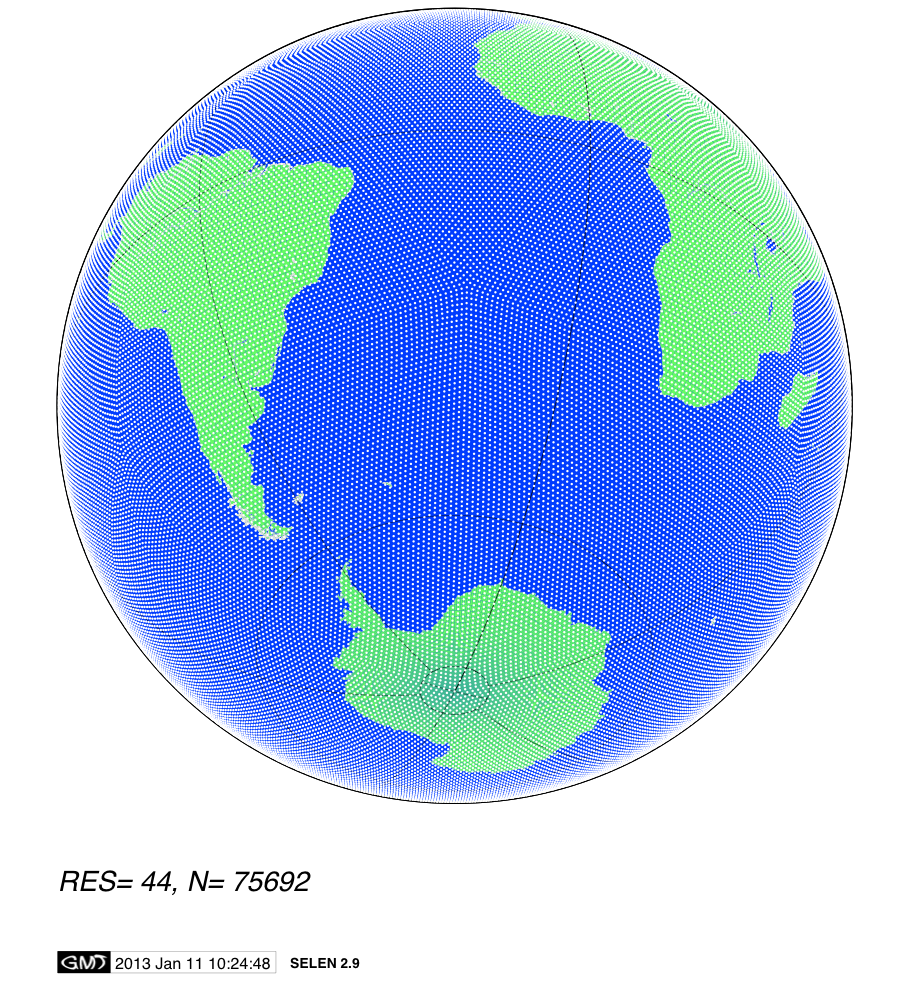
\includegraphics[angle=0,width=0.9\textwidth]{./Figures/px-sphere.png}
\vspace{0cm}
\caption[Tegmark icosahedral pixelization]{\small{Pixelization of the sphere for the \texttt{TEST} run ($\ell_{max}=128$, $R=44$). Data about the grid, including spherical coordinates of ``wet'' (oceanic, blue) and  ``dry'' (continental, green) pixels and postscript figures are found in folder \texttt{depot-TEST/px}. In \selens, wet pixels are separated by dry ones using the GMT program \texttt{gmtselect} \citep{Wessel_and_Smith_1998}. By default, \selen employs the full resolution coastlines of GMT (\texttt{-Df}), and dry (wet) pixels are selected using option \texttt{-Ns/k/s/k/s} (\texttt{-Nk/s/k/s/k}) of \texttt{gmtselect}}.}
\label{fig:pixelization} 
\end{center} 
\end{figure}
\newpage

\begin{figure}[h]
\begin{center}
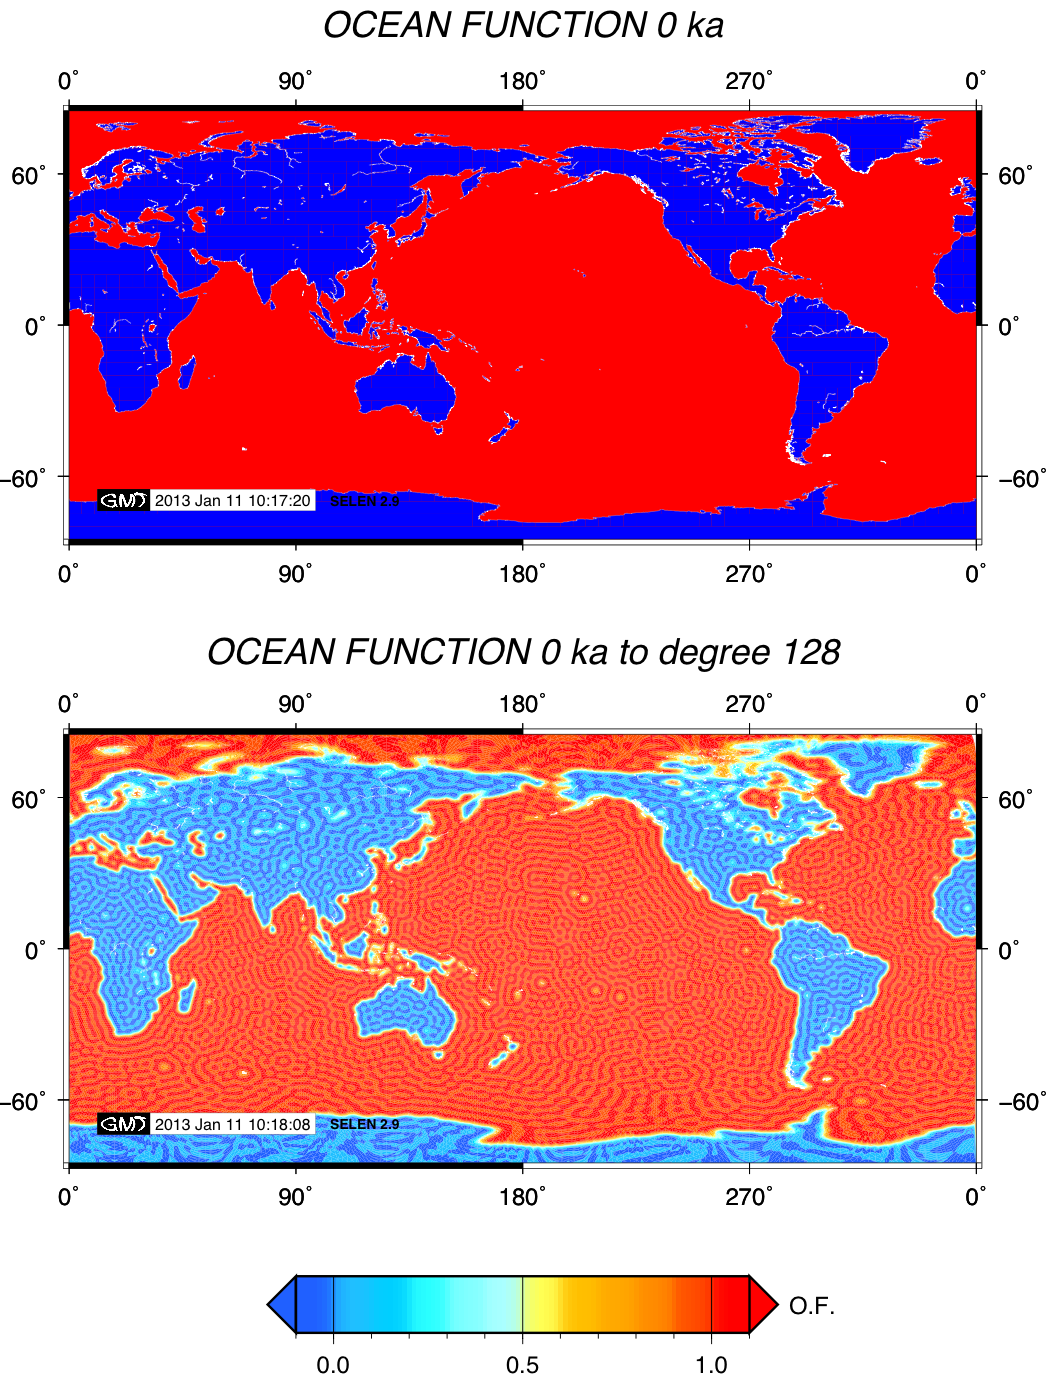
\includegraphics[angle=0,width=0.9\textwidth]{./Figures/of.png}
\vspace{0cm}
\caption[Ocean function]{\small{Original OF (top) and its reconstruction (bottom) obtained by synthesis of the SH coefficients to maximum degree $\ell_{max}=128$ (\texttt{TEST} run). All the OF data are stored in folder \texttt{depot-TEST/of}}.}
\label{fig:ocean-function}  
\end{center}
\end{figure}
\newpage

\begin{figure}[h]
\begin{center}
\vspace{-1em}
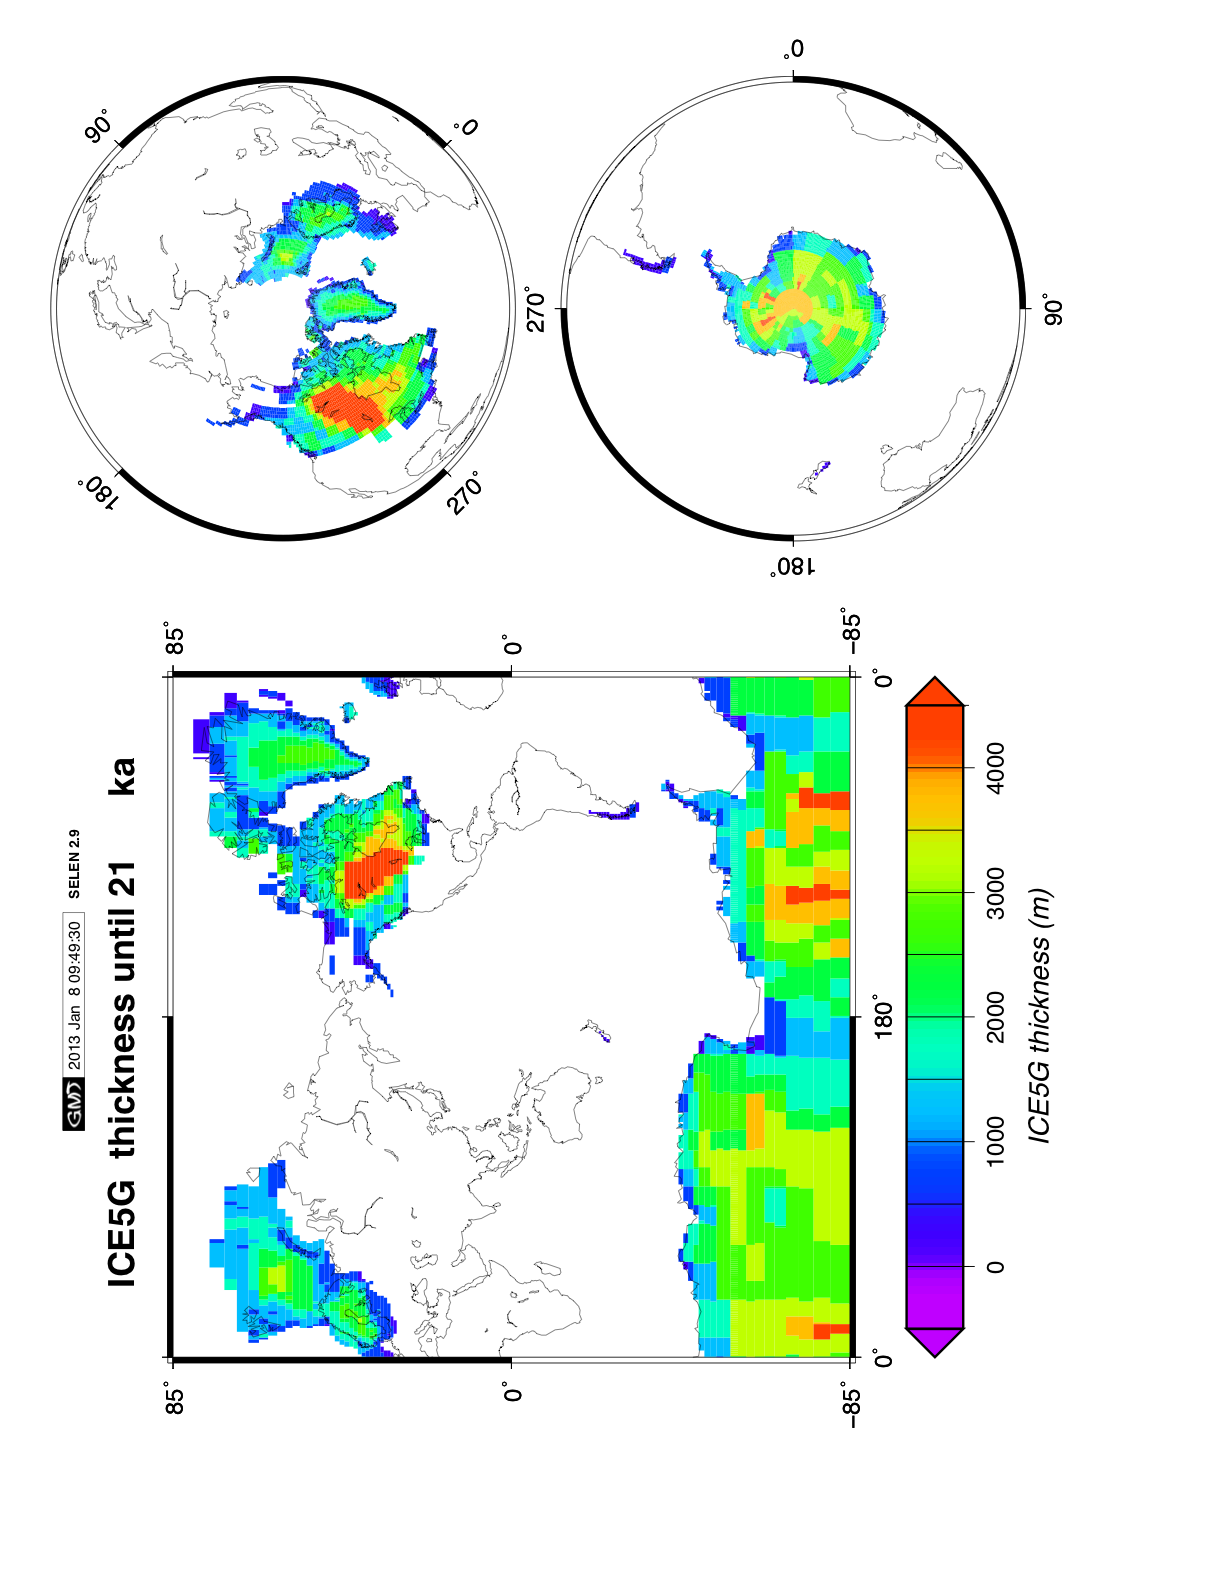
\includegraphics[width=0.71\textwidth, angle=-90]{./Figures/mapice00.png}\vspace{-4em}
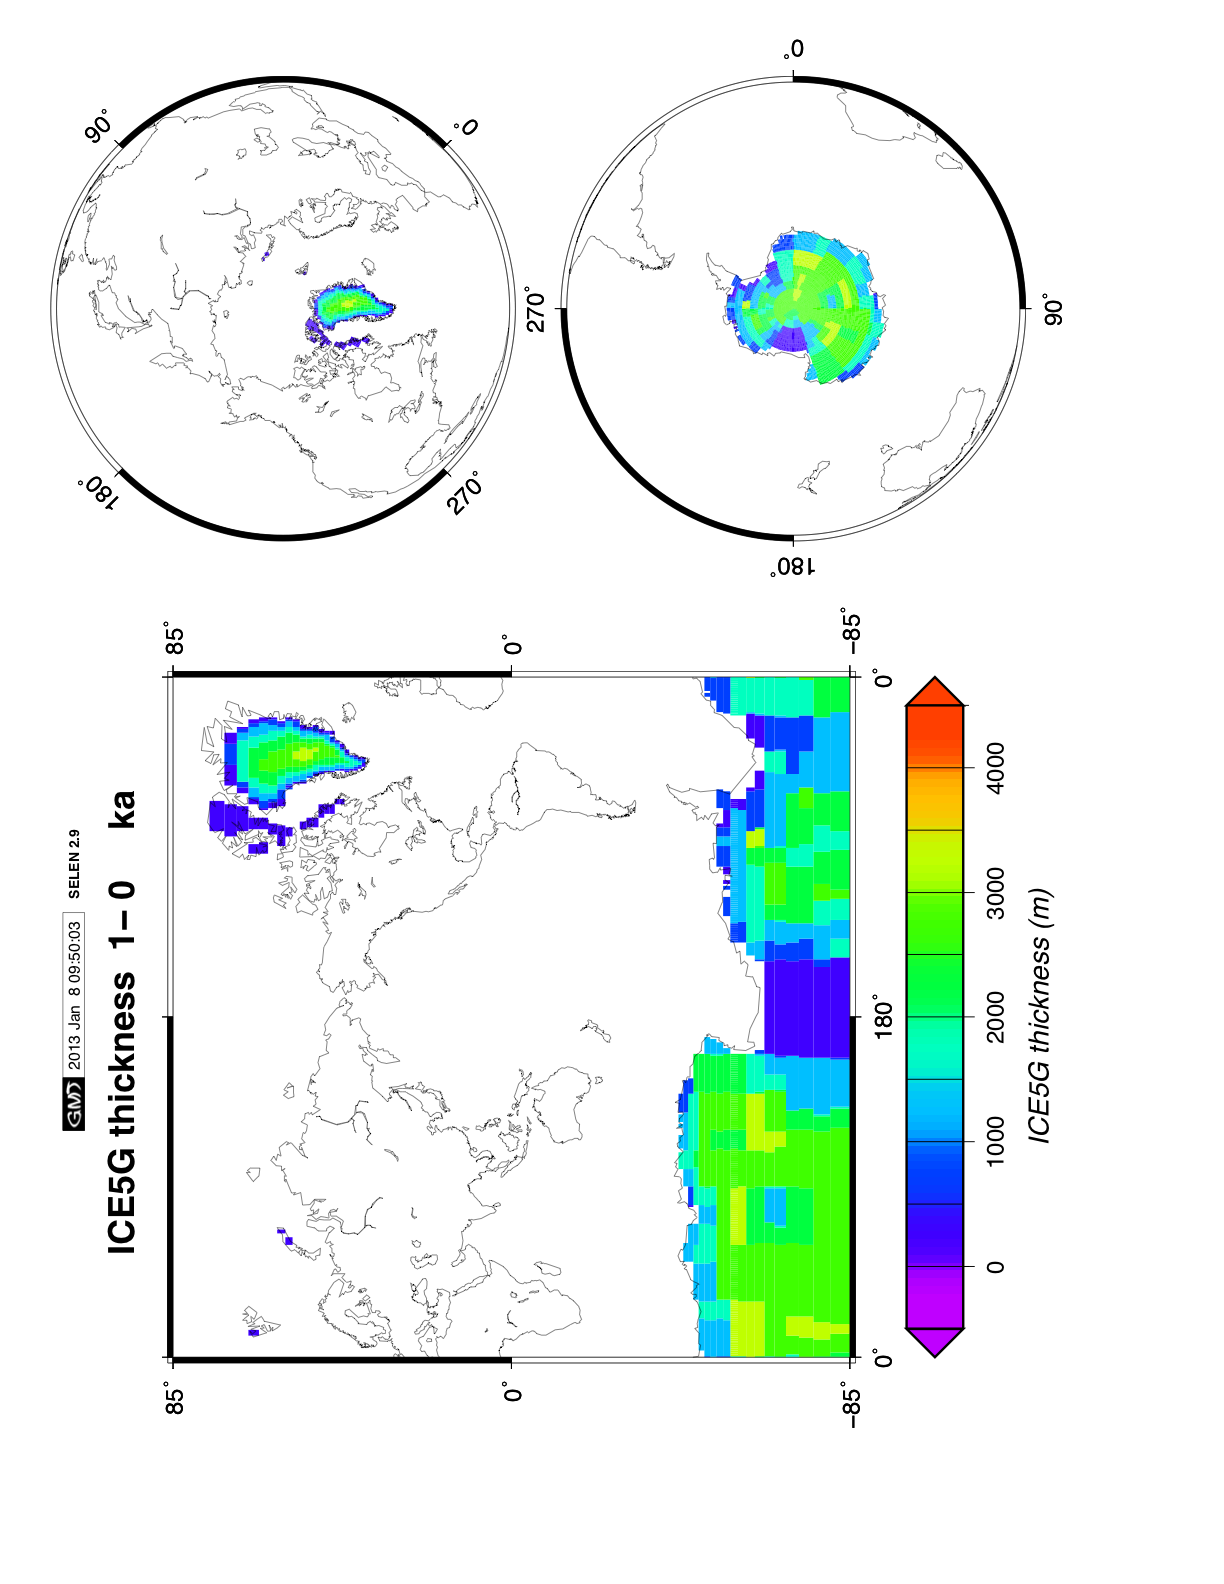
\includegraphics[width=0.71\textwidth, angle=-90]{./Figures/mapice21.png}\vspace{-2em}
\caption[Ice thickness distribution]{\small{Ice thickness $T(\omega,t)$ at the LGM ($21$ kyrs ago, top) and during the most recent 
time increment, between $1$ kyr BP and present time (bottom), according to model ICE--5G \citep{Peltier_2004} (\texttt{TEST run}). 
The time--history of the Equivalent Sea Level for this model is shown in Fig. \ref{fig:eustatic}. Maps
for all the other time steps between LGM and present are available in folder \texttt{depot-TEST/ICE5G/original}.}}
\label{fig:ice5g}
\end{center}
\end{figure}
\newpage

\begin{figure}[h]
\begin{center}
\vspace{1cm}
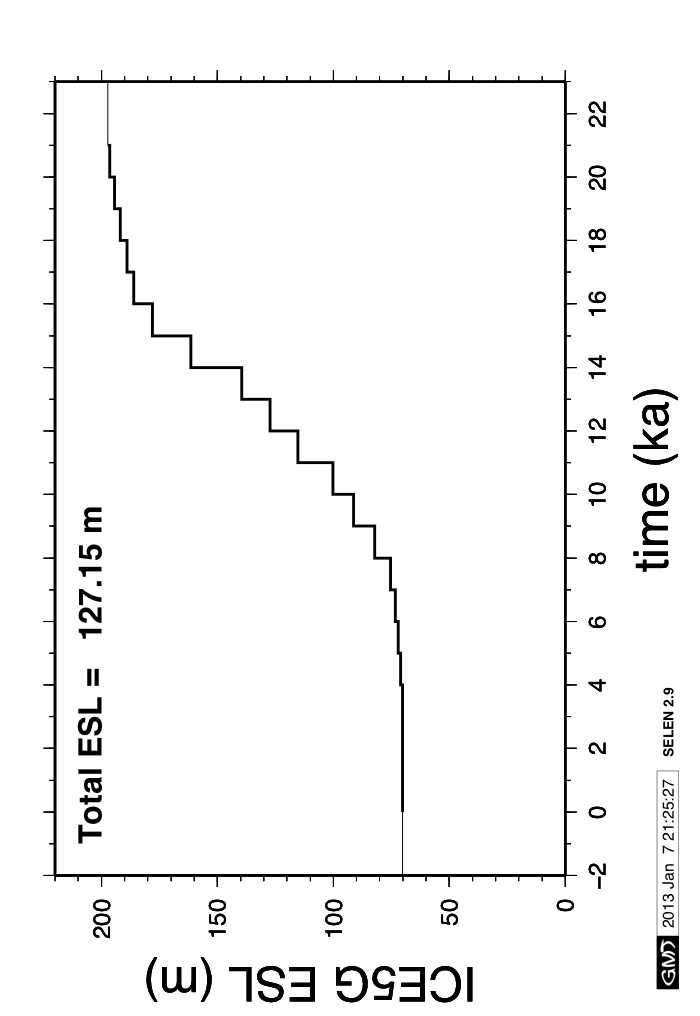
\includegraphics[width=0.6\textwidth, angle=-90]{./Figures/esl.png}
\caption[Equivalent Sea Level]{\small{Equivalent Sea Level for model ICE--5G \citep{Peltier_2004}
(\texttt{TEST} run). At a given time $t$ before present, 
$\textrm{ESL}(t)= (\rho_i/\rho_w)(V_{i}(t)-V_{i}(t_{p}))/A_{o})$, where  $V_{i}(t)$ is the ice volume, 
$V_{i}(t_{p})$ is present day volume, and $A_{o}$ is the area of the oceans surface. Hence, 
according to Eq.~(\ref{eustatic}), the plot of ESL mirrors that of $S^{E}(t)$. The total
ESL variation ($\sim 127$ m) represents the difference between ESL at the LGM ($21$ kyrs ago) and the present day value.}}
\label{fig:eustatic}
\end{center}
\end{figure}
\clearpage

%
% Table: Model parameters ... Table: Model parameters ... Table: Model parameters ... 
%
\begin{table}[p]
\begin{center}
\caption[Model parameters (\texttt{TEST} run)]{Model parameters for model VM2a, employed for the \texttt{TEST} run of \selens. These correspond to the model with \texttt{NV=3}, \texttt{CODE=2} and to the rheological profile described in file \texttt{DATA/vsc\_VM2a.dat}. This model represents a volume--averaged version of the VM2 viscosity profile associated with the ICE--5G model of \citet{Peltier_2004}.}
\begin{tabular}{lccccc}
\hline
Layer                           & Radius                        &Density                        &Shear modulus          &Viscosity                              &       Gravity\\
                                       & (km)                  &(kg m$^{-3}$)          &($\times 10^{11}$ Pa)  &($\times 10^{21}$Pa s) &(m s$^{-2}$)\\
\hline
{Lithosphere}                     & $6281$--$6371$        &$4120$                 &$0.73$                 &$\infty$                               &$9.707$\\
{Upper mantle}    & $5951$--$6281$        &$4120$                 &$0.95$                 &$0.5$                          &$9.672$\\
{Transition zone}                 & $5701$--$5951$        &$4220$                 &$1.10$                 &$0.5$                          &$9.571$\\
{Lower mantle}                    & $3480$--$5701$        &$4508$                 &$2.00$                 &$2.7$                          &$9.505$\\
{Core}                           & $0$--$3480$   & $10925$               &$0$                         &$0$                            &$10.622$\\
\hline
\label{table:vm2a}
\end{tabular}
\end{center}
\end{table}
\newpage

\begin{figure}[h]
\begin{center}
\vspace{1.2cm}
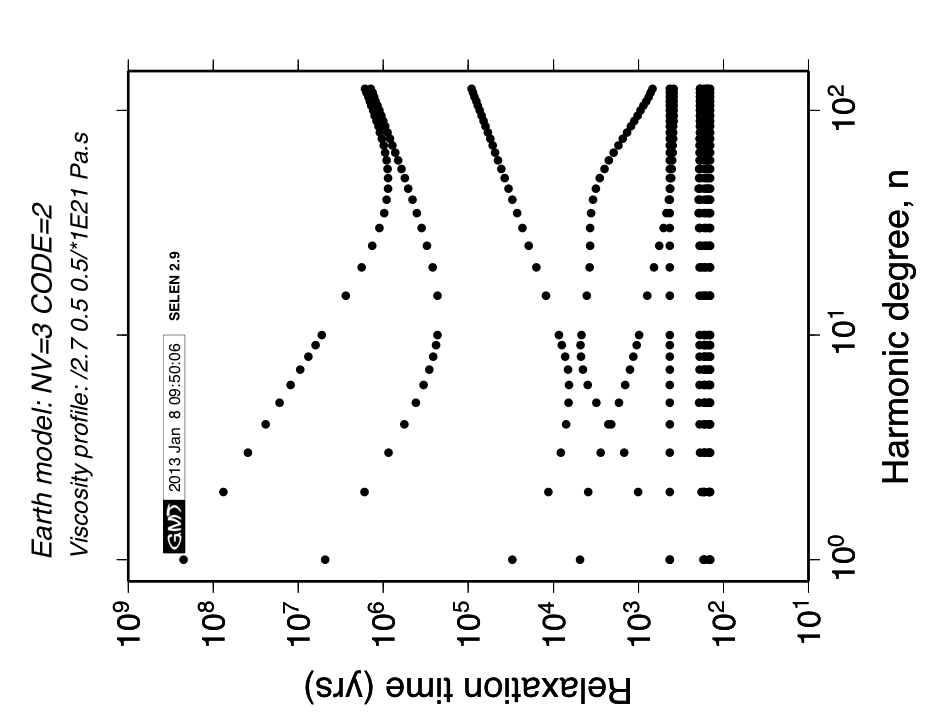
\includegraphics[width=0.90\textwidth, angle=-90]{./Figures/spectrum.png}
\caption[Relaxation spectrum]{\small{Isostatic relaxation spectrum for the rheological profile VM2a (see 
\texttt{TEST} run data in Table \ref{table:vm2a}), showing the relaxation times as a function of harmonic degree $\ell = n$ in the range $1\le \ell \le 128$. The spectrum data are stored in folder \texttt{depot-TEST/Love-Numbers-by-TABOO}. The physical meaning of the spectrum is discussed by e.g.~\citet{Peltier_1974}, \citet{Spada-2003a}, and \citet{Spada_etal_2011}}.}
\label{fig:spectrum}
\end{center}
\end{figure}
\newpage

\begin{figure}[h]
%\vspace{1cm}
\begin{center}
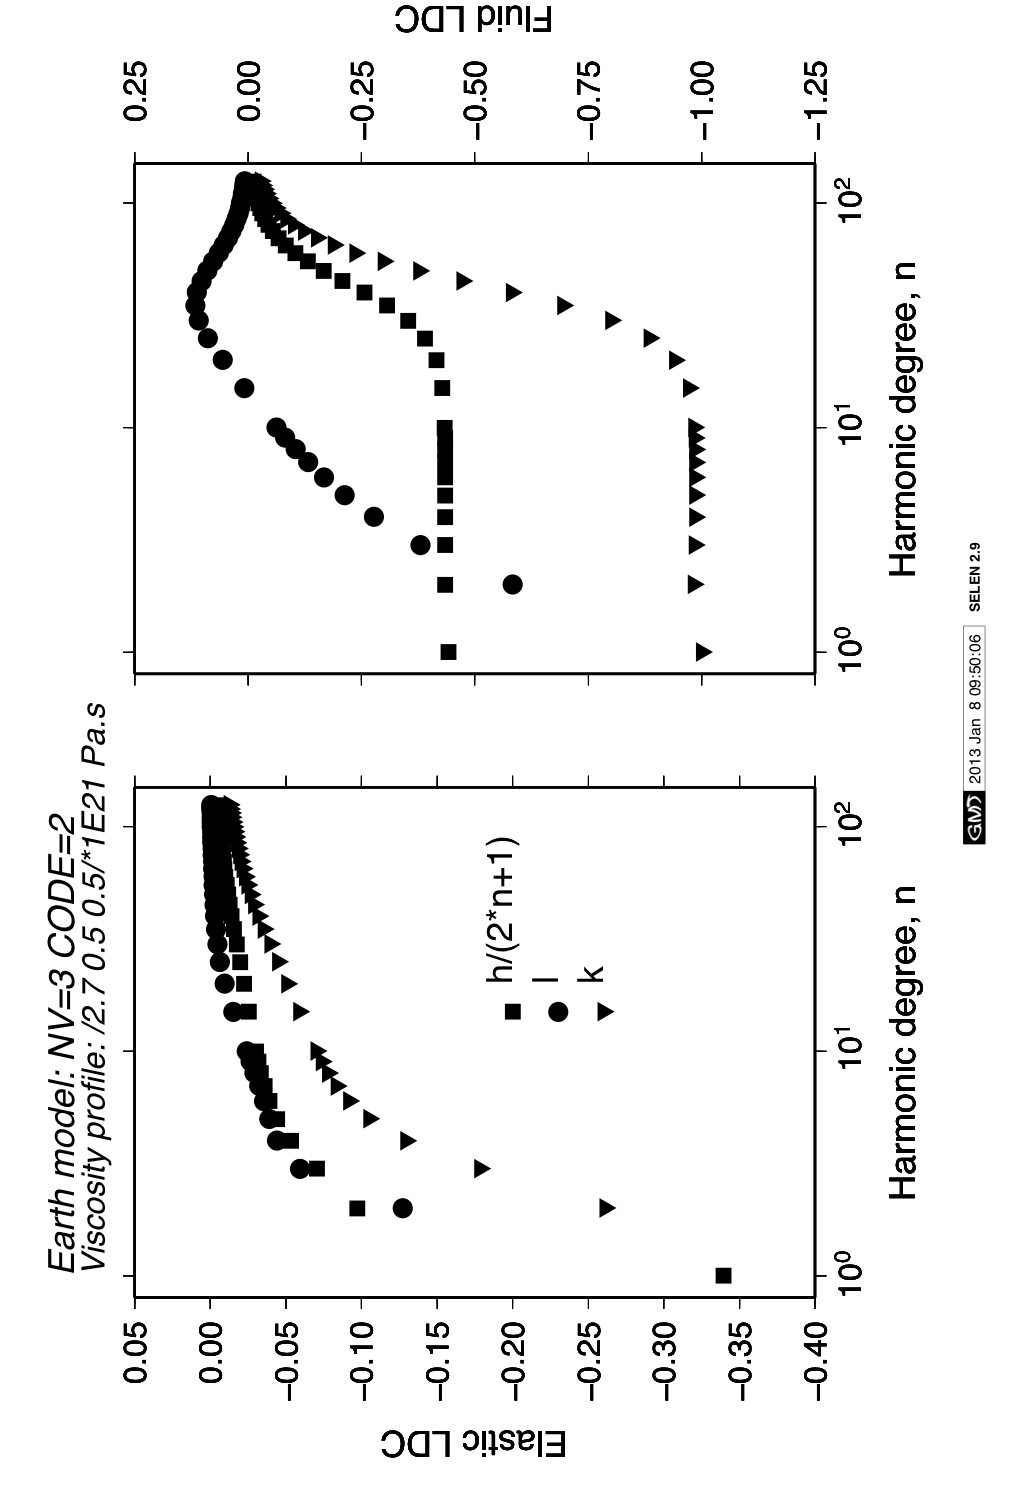
\includegraphics[width=0.68\textwidth, angle=-90]{./Figures/ela-flu.png}
\caption[Load---deformation coefficients (LDCs)]{\small{Elastic (left) and fluid (right) values of the LDCs 
$h$ (associated with vertical displacement), $l$ (horizontal displacement) and $k$ (incremental gravitational potential) for the rheological model VM2a in the \texttt{TEST} run (see Table~\ref{table:vm2a}), as a function of harmonic degree $\ell$. LDC $h$ is normalized by $(2\ell +1)$. For the definition of the LDCs
see e.g.~\citet{Spada-2003a}, and \citet{Spada_etal_2011}}.}
\label{fig:ldcs}
\end{center}
\end{figure}
\newpage

\begin{figure}[h]
\begin{center}
%\vspace{1cm}
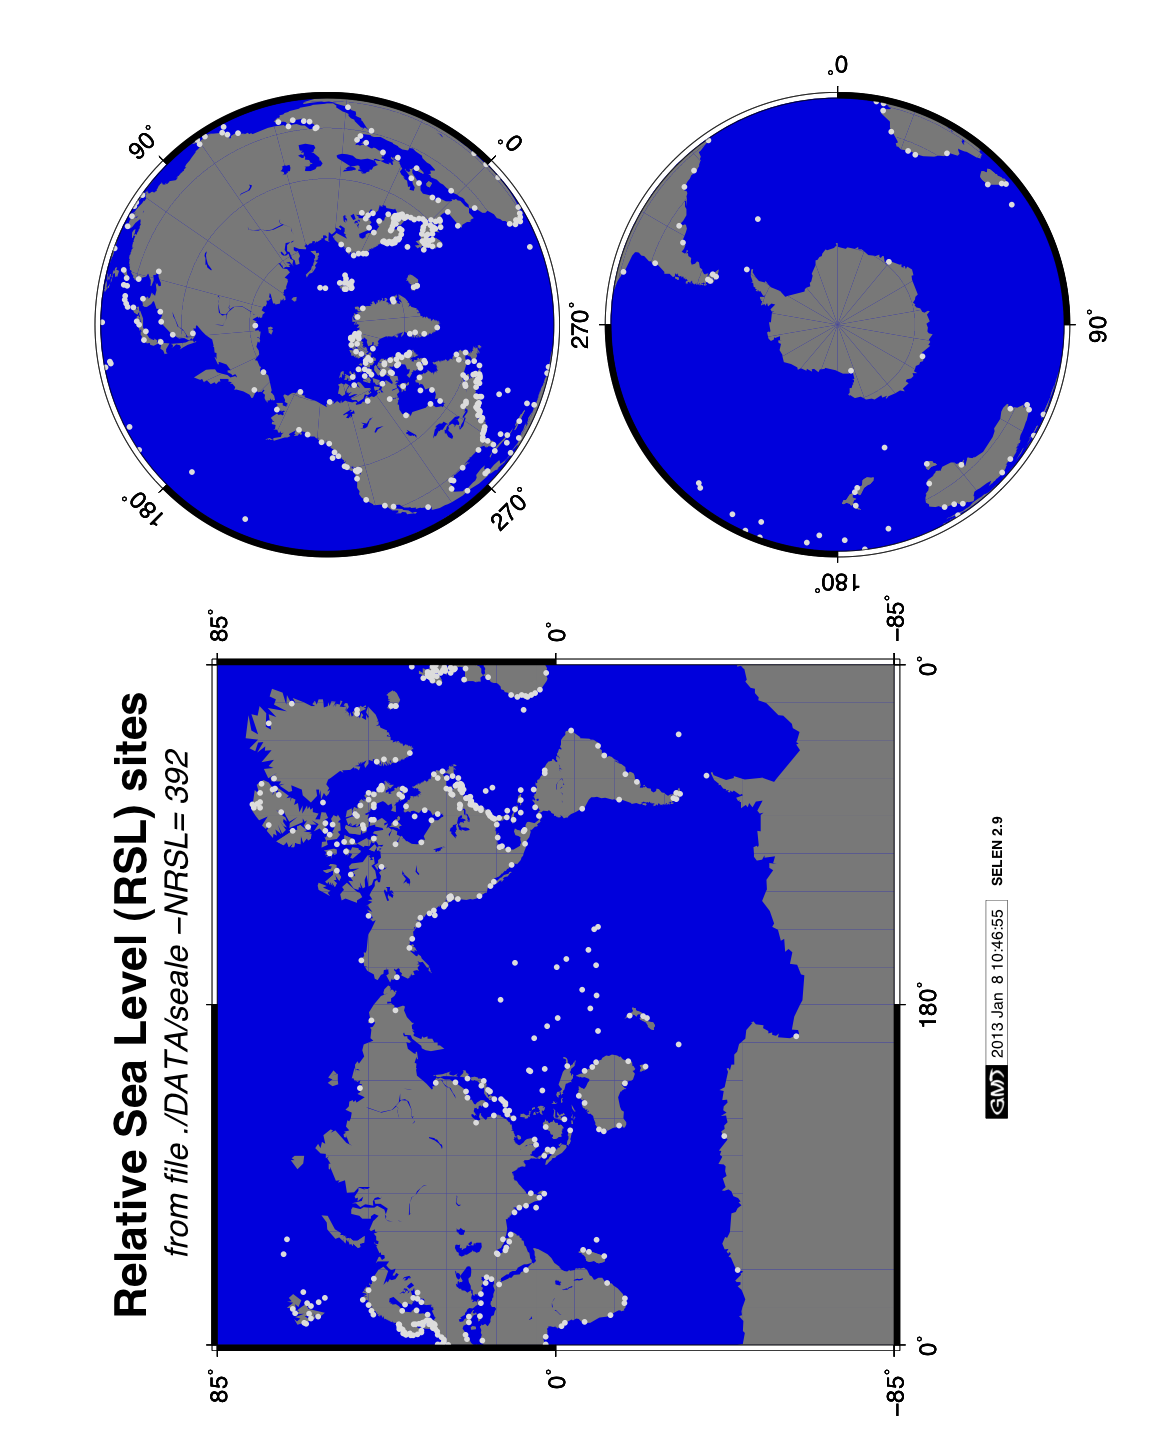
\includegraphics[width=0.82\textwidth, angle=-90]{./Figures/maprsl.png}
\caption[RSL sites]{\small{Geographical distribution of the $392$ sites in file \texttt{sealevel.dat}, from which information about the history of RSL during the last $\sim 15,000$ years is available. This plot 
and more data about these sites are available from de folder \texttt{depot-TEST/rsl/rsl-sites}}.}
\label{fig:rsl-sites}
\end{center}
\end{figure}
\clearpage

\begin{figure}[h]
\begin{center}
\vspace{-1.5cm}
\noindent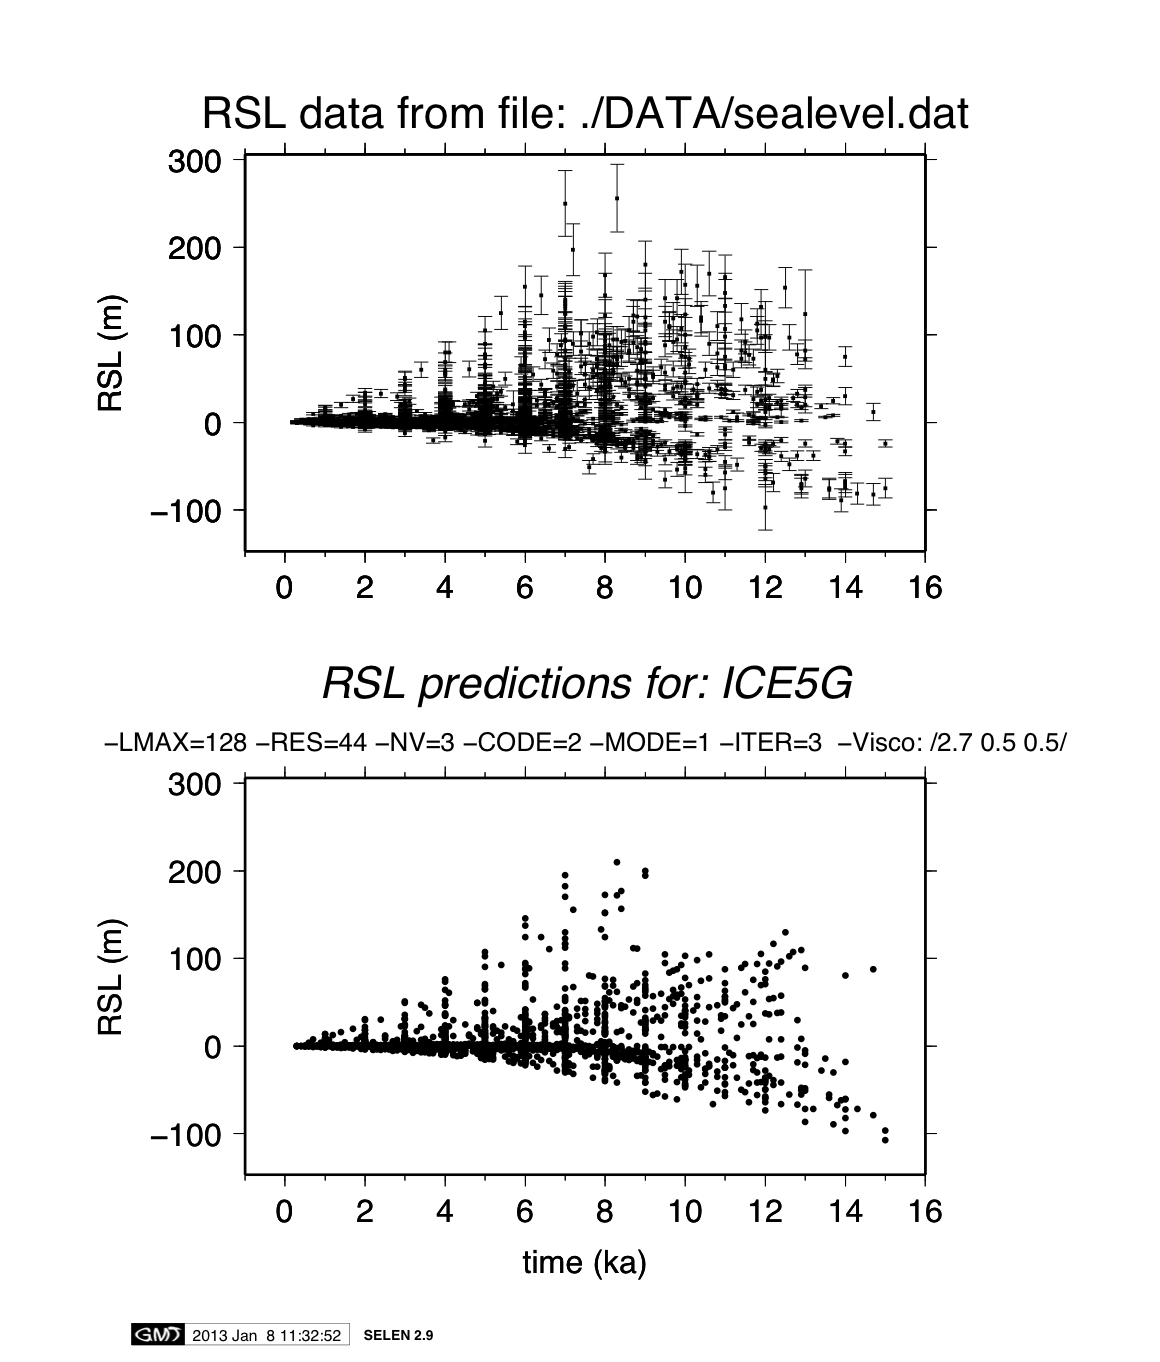
\includegraphics[width=0.95\textwidth, angle=0]{./Figures/scatter-plot.png}
\caption[RSL scatterplot]{\small{Scatterplot showing RSL observations (top) from sites of the compilation of 
\citet{Tushingham_and_Peltier_1992,Tushingham_and_Peltier_1993}. 
RSL predictions at all sites, obtained solving the SLE in our \texttt{TEST} run of \selens, 
are shown in the bottom frame. Data are stored in folder \texttt{depot-TEST/rsl/rsl-scplot}.}}
\label{fig:rsl-scatterplot}
\end{center}
\end{figure}
\newpage

\begin{figure}[h]
\begin{center}
\vspace{0.6cm}
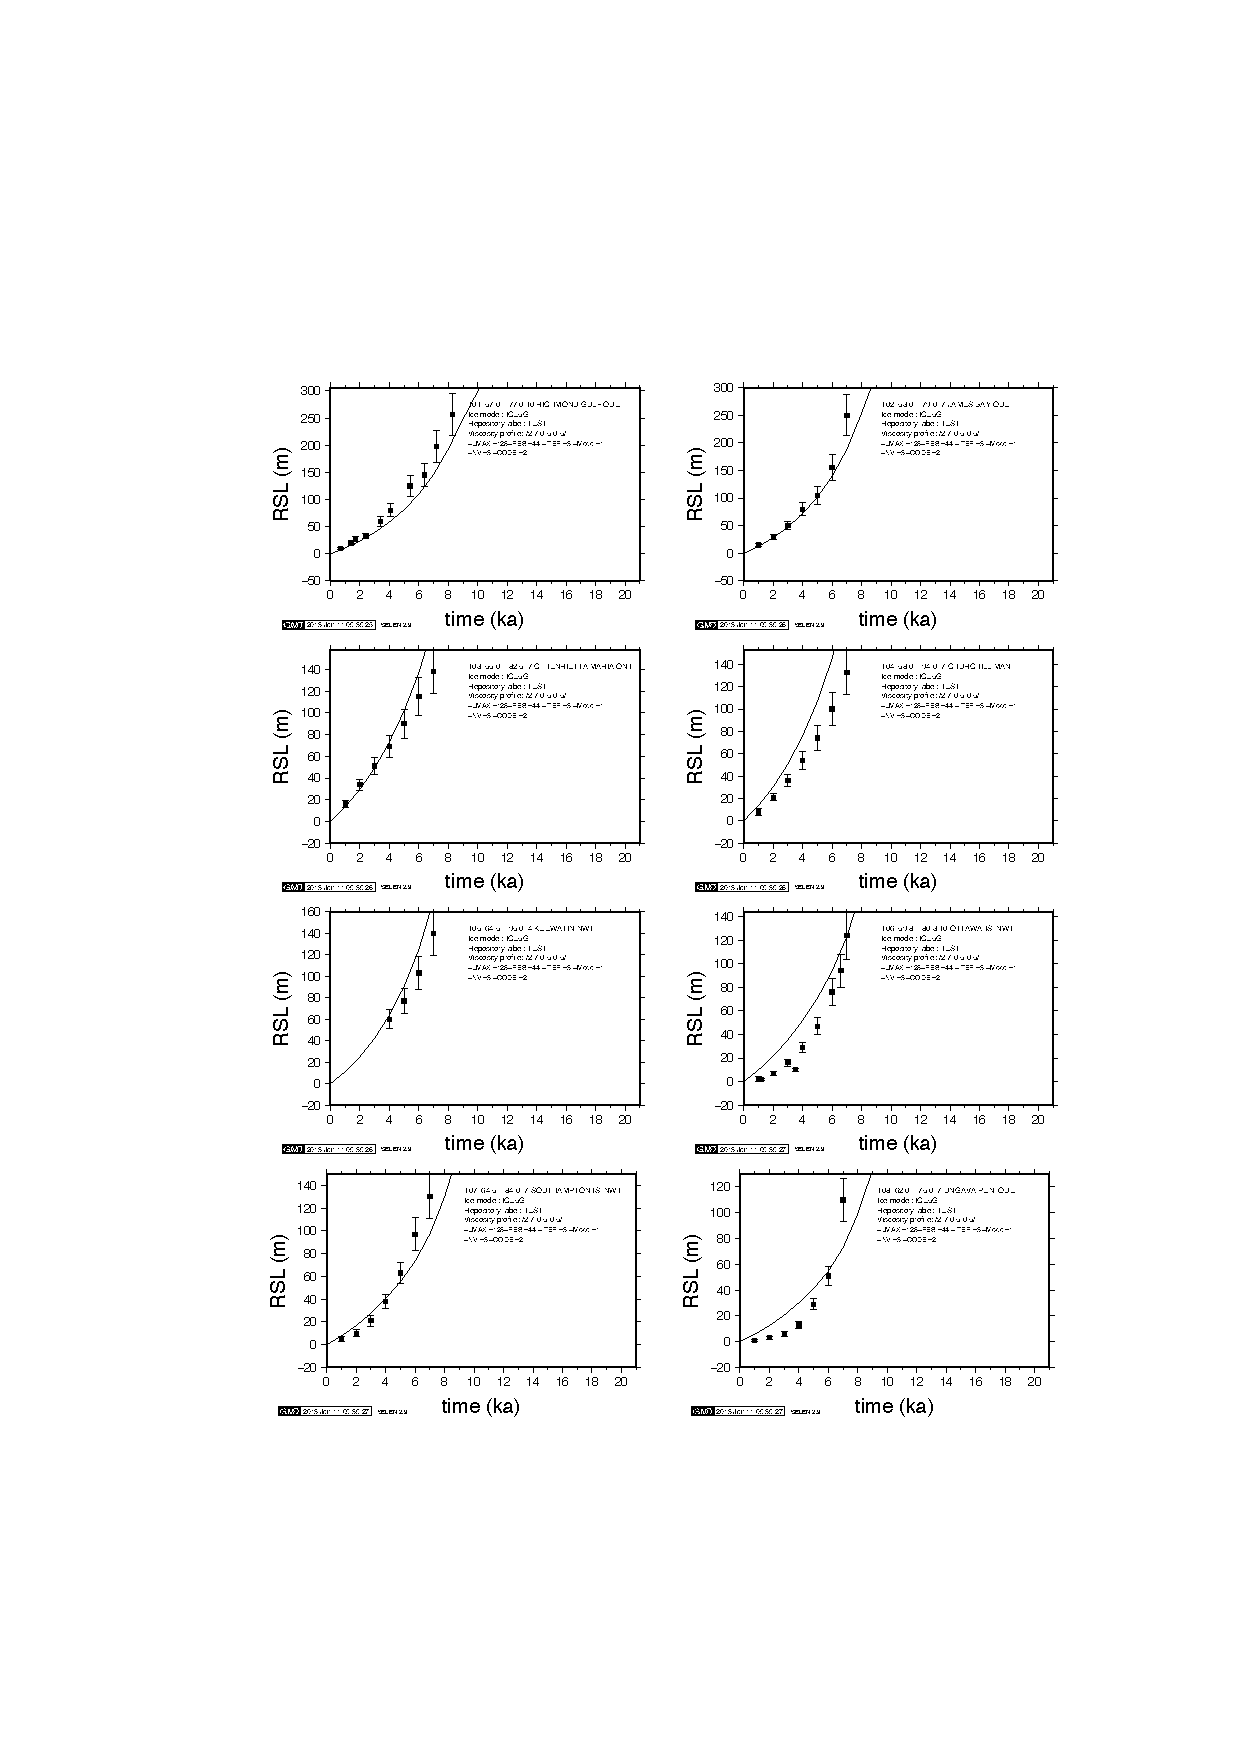
\includegraphics[width=0.9\textwidth,angle=0]{./Figures/rsl-1.pdf}
\caption[Hudson bay RSL curves]{\small{RSL observations (with error bars) pertaining to the eight sites of Hudson bay in file \texttt{sealevel.dat}, compared with \selen predictions (solid curves). Basic parameters 
for the \texttt{TEST} run are summarized in each frame. Postscript and PDF figures are located  
in folders \texttt{depot-TEST/rsl/rsl-curves/ps} and \texttt{depot-TEST/rsl/rsl-curves/pdf}, respectively.}}
\label{fig:rsl-1}
\end{center}
\end{figure}
\newpage

\begin{figure}[h]
\begin{center}
\vspace{0.6cm}
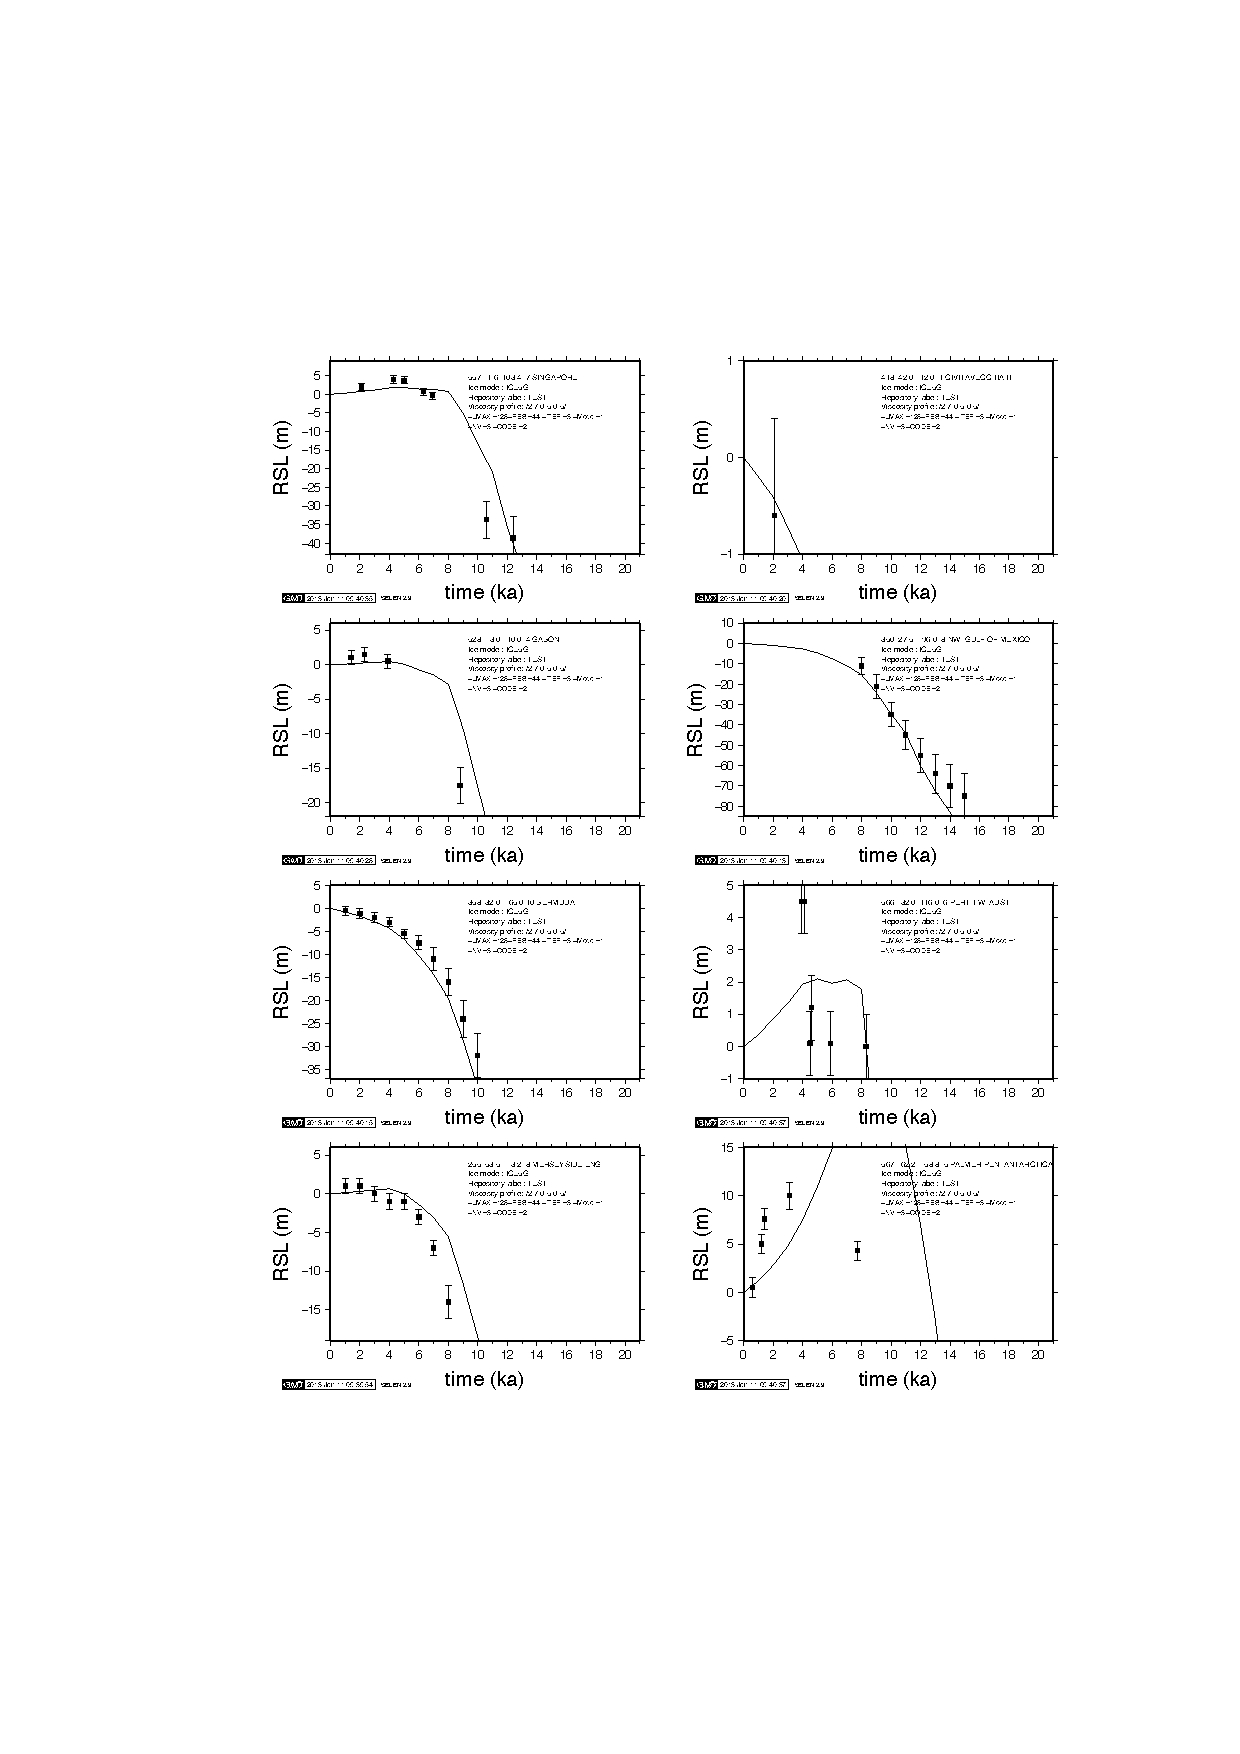
\includegraphics[width=0.9\textwidth,angle=0]{./Figures/rsl-2.pdf}
\caption[Miscellanea RSL curves]{\small{RSL curves at eight miscellanea sites located in the far field of the former ice sheets: Singapore, Civitavecchia (Italy), Gabon, NW Gulf of Mexico, Bermuda, Perth W. Australia, Merseyside (England), and Palmer peninsula (Antarctica). All the RSL predictions for the
\texttt{TEST} run are found in \texttt{depot-TEST/rsl/rsl-curves}}.}
\label{fig:rsl-2}
\end{center}
\end{figure}
\newpage

\begin{figure}[h]
\begin{center}
\vspace{0cm}
\noindent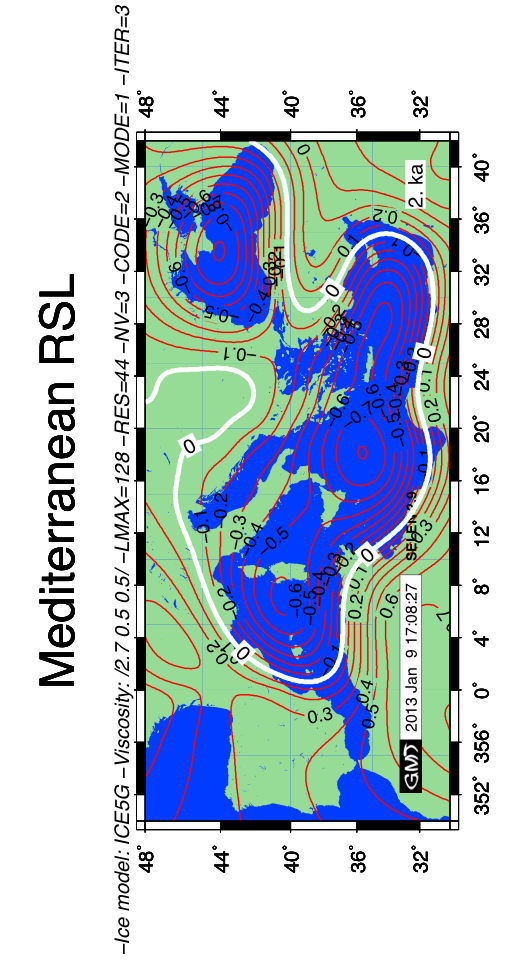
\includegraphics[width=0.71\textwidth, angle=0]{./Figures/rslc-map.png}
\vspace{0cm}
\caption[Holocene RSL in the Mediterranean Sea]{\small{Example of RSL contour plot for the Mediterranean region, obtained at time $2$ kyrs BP setting the configurations file \texttt{DATA/rsl-region.dat} (RSL is given in units of meters). The computations are based on the \selen parameters employed in the \texttt{TEST} run (ice model ICE--5G and rheological parameters in Table \ref{table:vm2a})}.}
\label{fig:med-rslc}
\end{center}
\end{figure}
\newpage

\begin{figure}[h]
\begin{center}
%\vspace{2cm}
\noindent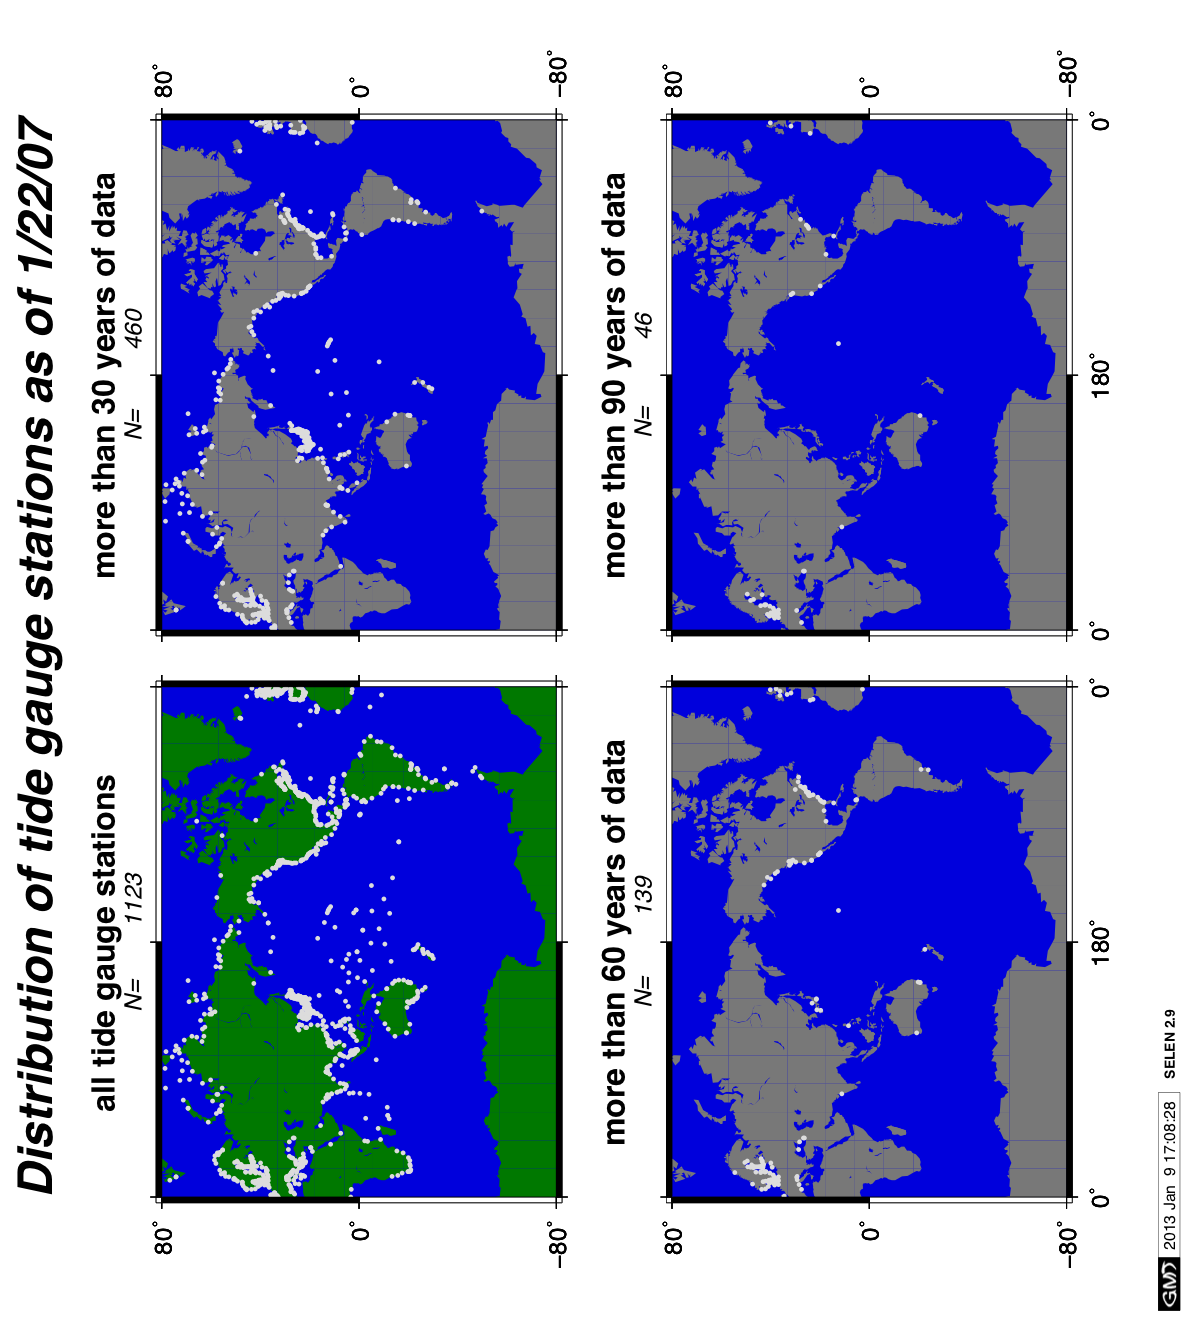
\includegraphics[width=0.90\textwidth, angle=-90]{./Figures/map-tgauges.png}
\caption[Tide gauges locations]{\small{Geographical distribution of the TGs considered in run \texttt{TEST}, according to the number of annual records available from each station in the user--supplied input file \texttt{DATA/rlr-trends.txt}. Data and plots for this analysis are stored in folder 
in \texttt{depot-TEST/tgauges/tgauges-sites} after the execution of \selens.}}
\label{fig:tg-distribution}
\end{center}
\end{figure}
\newpage

\begin{table}[h]
\caption[Geodetic variations at TGs (\texttt{TEST} run)]{\small{Present--day trends of GIA--induced \sealevel change 
(\texttt{s-dot}), 
sea surface variation (\texttt{n-dot}), and vertical velocity of the solid Earth (\texttt{u-dot}), expressed in units of millimeters 
per year, at RLR (Revised Local Reference) 
PSMSL TGs in the user--supplied file \texttt{DATA/rlr-trends.txt} employed for the \texttt{TEST} run). The table 
also contains basic information on the TGs and an header with a short summary of the run parameters. 
This is an excerpt of the ASCII table \texttt{depot-TEST/tauges/tgauges-predictions/ptidegauges}}.}
{\color{black}{\tiny\begin{verbatim}

 2013.01.09 time=17.09.10
 Ice model: ice5g.dat
 Number of mantle layers:            3
 Model code (see TABOO User guide):            2
 Viscosity model: ./VSC/vsc_VM2a.dat
 Thickness of the lithosphere (km): '90.'
 Viscosity (bottom-to-top, Haskell units) '2.7'
 Viscosity (bottom-to-top, Haskell units) '0.5'
 Viscosity (bottom-to-top, Haskell units) '0.5'
 SLE iterations:            3
 SLE mode of solution:            1
 Maximum harmonic degree:          128
 Tegmark resolution:           44
------------------------------------------------------------------------------------------------------------------------------- 
  PSMSL    yrs    range       trend  error     lon       lat       s-dot     n-dot     u-dot    PSMSL station name
  code             yrs            mm/yr        deg       deg       mm/yr     mm/yr     mm/yr    ==================
-------------------------------------------------------------------------------------------------------------------------------  
 010/001   40  1957 - 2003     2.23   0.46   338.067    64.150     0.147    -0.210    -0.357    REYKJAVIK                     
 010/011    6  1958 - 1965     8.07   8.35   337.567    63.833     0.274    -0.219    -0.494    GRINDAVIK                     
 015/011   22  1958 - 2001     1.50   0.34   353.233    62.017     0.645    -0.188    -0.826    TORSHAVN                      
 025/001   44  1949 - 2003    -2.65   0.42    14.250    78.067    -0.888     0.057     0.974    BARENTSBURG                   
 025/002   42  1949 - 1993    -1.36   0.46    14.250    78.067    -0.888     0.057     0.974    BARENTSBURG II (SPITSBERGEN)  
 025/021   20  1977 - 2004    -3.10   0.64    11.933    78.933    -0.312     0.031     0.354    NY-ALESUND                    
 030/001   36  1953 - 1989    -1.26   0.62    62.583    76.200    -2.878     0.093     3.070    RUSSKAYA GAVAN                
 030/003   36  1953 - 1989    -1.28   0.62    62.583    76.183    -2.867     0.093     3.059    RUSSKAIA GAVAN II             
 030/007   19  1960 - 1978     2.43   2.52    60.217    69.600    -0.219    -0.064     0.148    BELYI NOS                     
 030/014   28  1962 - 1990    -4.89   1.07    58.050    80.617    -2.807     0.070     2.992    KRENKELIA (HEISA OSTROV)      
 030/016   23  1950 - 1976    -3.10   1.91    52.700    72.367    -2.132     0.101     2.305    MALYE KARMAKULY               
 030/018   48  1952 - 2005     3.14   0.67    33.050    68.967    -3.090     0.290     3.403    MURMANSK                      
 ...
 [omitted records]
 ...
 240/001   10  1896 - 1913     1.29   1.43     9.367    41.233     0.267    -0.317    -0.587    LA MADDALENA                  
 240/011   26  1897 - 1934     1.64   0.39     9.167    39.200     0.250    -0.324    -0.577    CAGLIARI                      
 250/001   23  1897 - 1921     1.60   0.59     8.017    43.867     0.103    -0.297    -0.402    PORTO MAURIZIO                
 250/011   78  1884 - 1992     1.20   0.07     8.900    44.400     0.070    -0.290    -0.362    GENOVA                        
 250/031   21  1897 - 1920     1.10   0.68    11.817    42.050     0.202    -0.308    -0.512    CIVITAVECCHIA                 
 250/041   11  1901 - 1921     2.28   1.42    14.267    40.867     0.199    -0.314    -0.514    NAPOLI (ARSENALE)             
 250/051   18  1897 - 1921     2.18   0.66    14.267    40.867     0.199    -0.314    -0.514    NAPOLI (MANDRACCIO)           
 250/061    9  1951 - 1964    -2.69   3.08    15.650    38.100     0.276    -0.326    -0.605    REGGIO CALABRIA               
 260/011   15  1897 - 1919     0.98   0.63    13.333    38.133     0.250    -0.326    -0.579    PALERMO                       
 260/028    9  1957 - 1968     8.54   3.68    15.300    36.667     0.314    -0.329    -0.647    CAPO PASSERO                  
 260/031   12  1960 - 1971    -3.02   2.78    15.133    37.500     0.289    -0.328    -0.620    CATANIA                       
 265/001   11  1991 - 2004     0.63   2.62    14.517    35.900     0.290    -0.329    -0.622    VALLETTA                      
 270/006    6  1906 - 1911    -3.49   6.73    17.267    40.433     0.179    -0.313    -0.494    TARANTO                       
 270/011    4  1961 - 1970    -0.58   1.63    18.500    40.133     0.176    -0.314    -0.492    OTRANTO                       
 270/035    3  1970 - 1972     9.00   2.89    12.283    44.500     0.082    -0.284    -0.367    PORTO CORSINI                 
 270/041   18  1889 - 1913     2.04   1.20    12.350    45.417     0.039    -0.273    -0.314    VENEZIA (ARSENALE)            
 270/051   45  1872 - 1919     2.55   0.42    12.333    45.417     0.039    -0.273    -0.314    VENEZIA (S.STEFANO)           
 270/054   82  1909 - 2000     2.39   0.16    12.333    45.433     0.038    -0.273    -0.313    VENEZIA (PUNTA DELLA SALUTE)  
 270/061   96  1905 - 2006     1.17   0.12    13.750    45.650     0.037    -0.268    -0.307    TRIESTE                       
 ...
 [omitted records]
 ...
 970/211    6  1962 - 2005     2.50   1.19   227.033    69.417     1.393     0.104    -1.295    TUKTOYAKTUK                   
 A  /001    4  1967 - 1977     0.92   6.43   303.083   -63.300    -1.313    -0.050     1.272    BAHIA ESPERANZA               
 A  /003   43  1960 - 2004     1.57   0.37   295.733   -65.250    -1.326     0.030     1.361    ARGENTINE ISLANDS             
 A  /005   15  1985 - 2002     5.75   1.85   300.367   -62.483    -1.304    -0.061     1.251    PUERTO SOBERANIA              
 A  /024    8  1958 - 1978    -1.22   1.82   297.133   -64.900    -1.454     0.020     1.480    ALMIRANTE BROWN               
------------------------------------------------------------------------------------------------------------------------------- 
\end{verbatim} }}
\label{tab:test-run-tg}
\end{table}  
\newpage

\begin{figure}[h]
\begin{center}
%\vspace{-0.8cm}
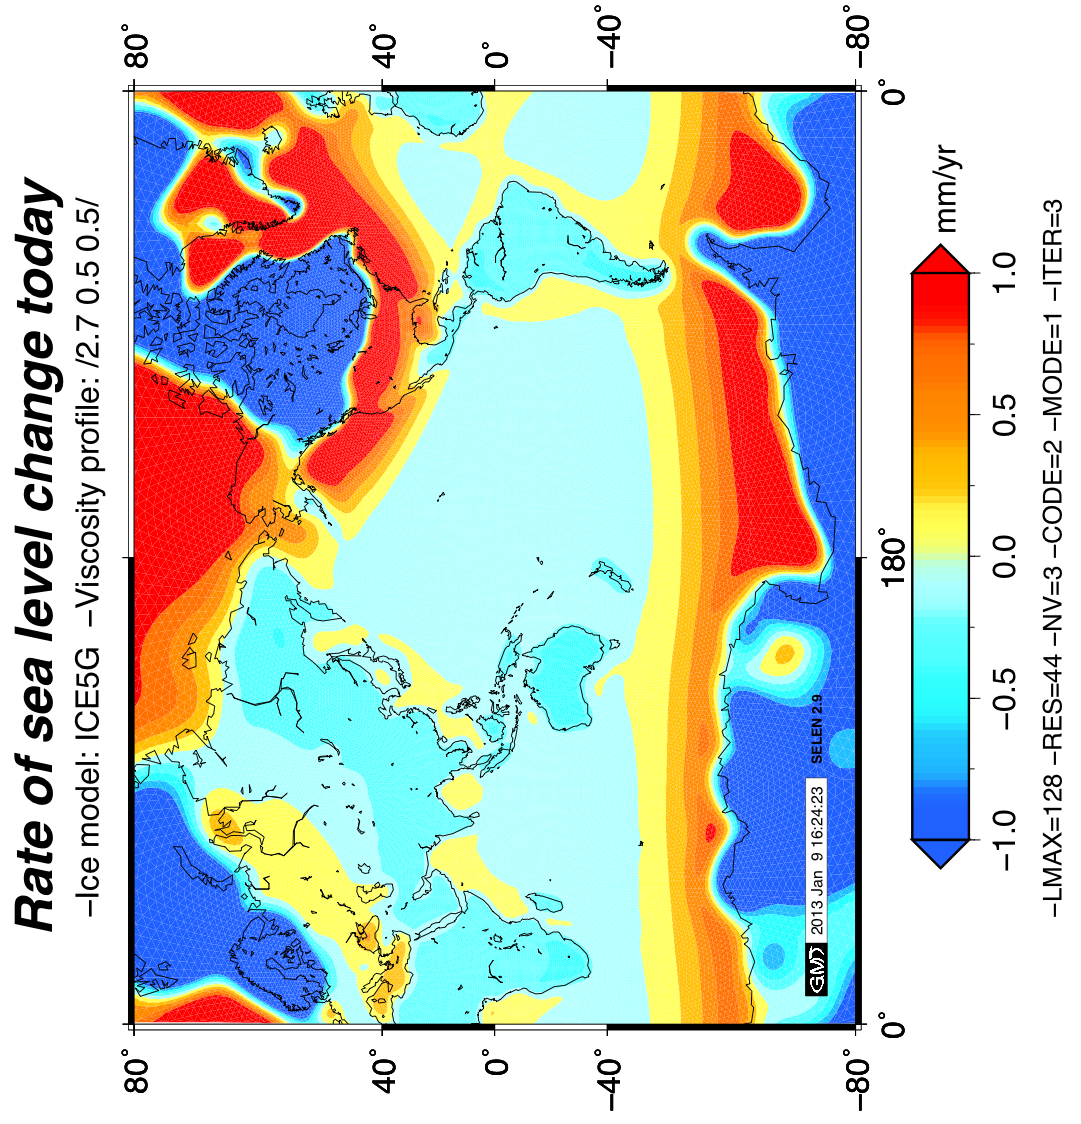
\includegraphics[width=0.9\textwidth, angle=-90]{./Figures/sdotmap.png}
%\vspace{-0.8cm}
\caption[Relative \sealevel fingerprint]{\small{Global map showing the present--day rate of \sealevel change (\textit{\sealevel fingerprint}) associated with GIA ($\dot S$)
for our \texttt{TEST} run. Data and plots for this analysis are found in folder \texttt{depot-TEST/gmaps}. In this map, the $\dot S$ values vary in the range $[-17.01/+3.67]$ mm/yr.}}
\label{fig:sdot}
\end{center}
\end{figure}
\newpage

\begin{figure}[h]
\begin{center}
%\vspace{-0.8cm}
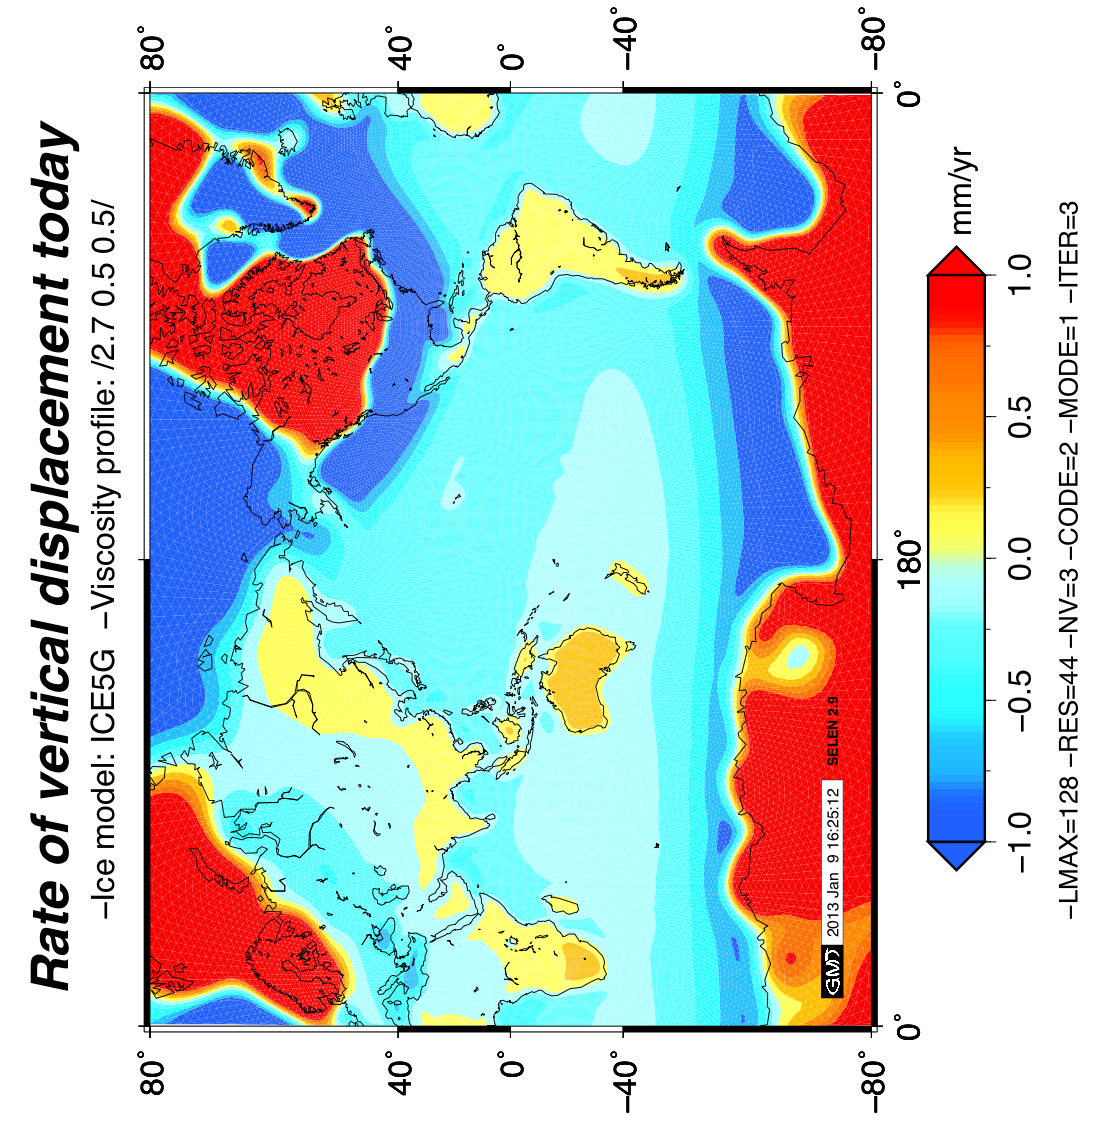
\includegraphics[width=0.9\textwidth, angle=-90]{./Figures/udotmap.png}
%\vspace{-0.8cm}
\caption[Vertical velocity fingerprint]{\small{Global map of the GIA--induced vertical velocity ($\dot U$) for the \texttt{TEST} run. Subsiding and uplifting areas are shown by blue and red hues, respectively. 
The range of the $\dot U$ values is $[-3.53/+19.24]$ mm/yr.}}
\label{fig:udot}
\end{center}
\end{figure}
\newpage

\begin{figure}[h]
\begin{center}
%\vspace{-0.8cm}
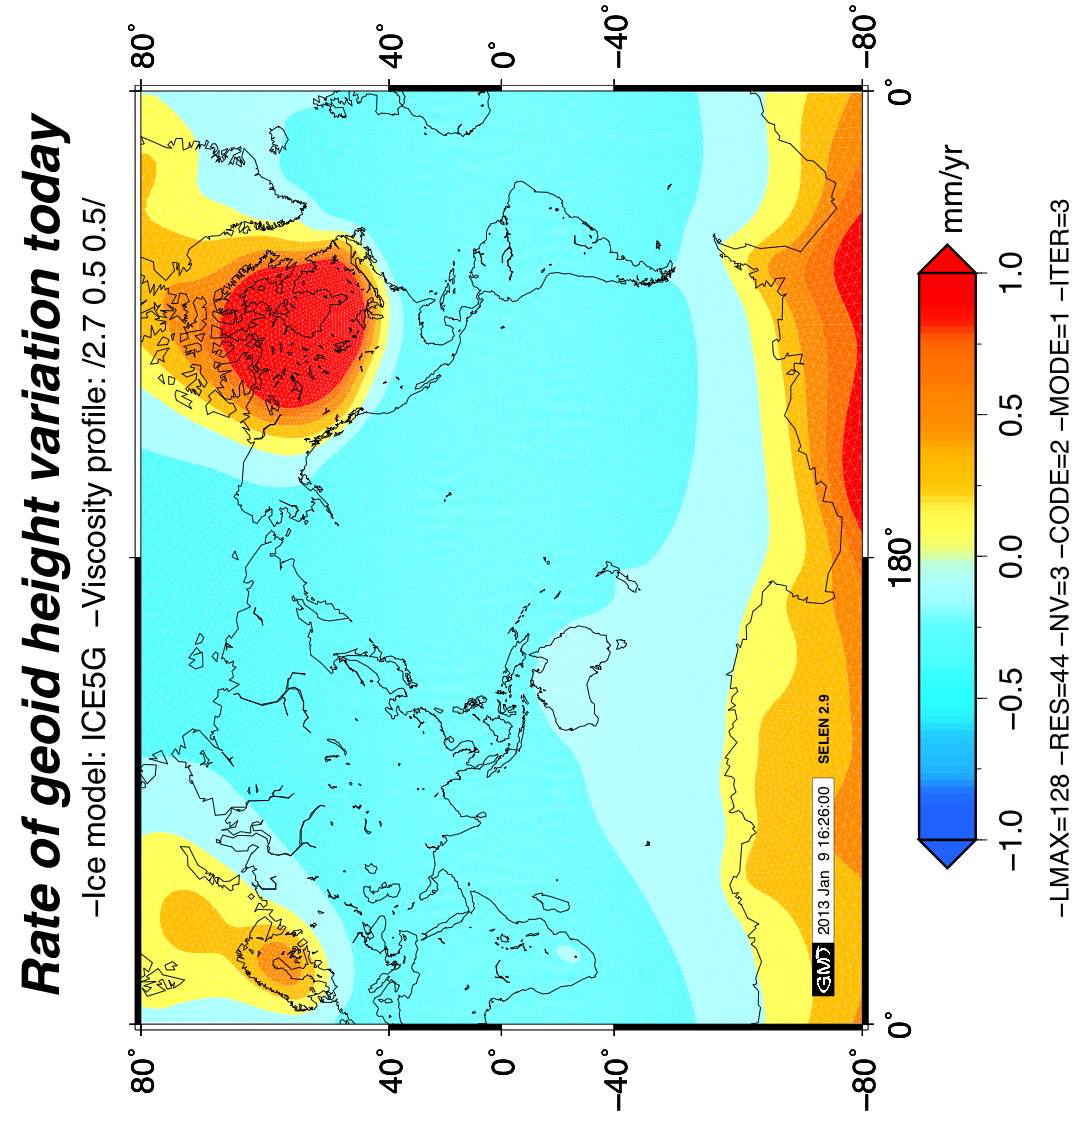
\includegraphics[width=0.9\textwidth, angle=-90]{./Figures/ndotmap.png}
%\vspace{-0.8cm}
\caption[Absolute \sealevel fingerprint]{\small{Rate of sea surface variation induced by GIA (\textit{absolute} \sealevel variation), relative to the Earth's center of mass ($\dot N$), for run \texttt{TEST}. In this map, the range of variation of $\dot N$ is $[-0.40/+2.35]$ mm/yr.}}
\label{fig:ndot}
\end{center}
\end{figure}
\newpage

\begin{figure}[p]
\begin{center}
%\vspace{2cm}
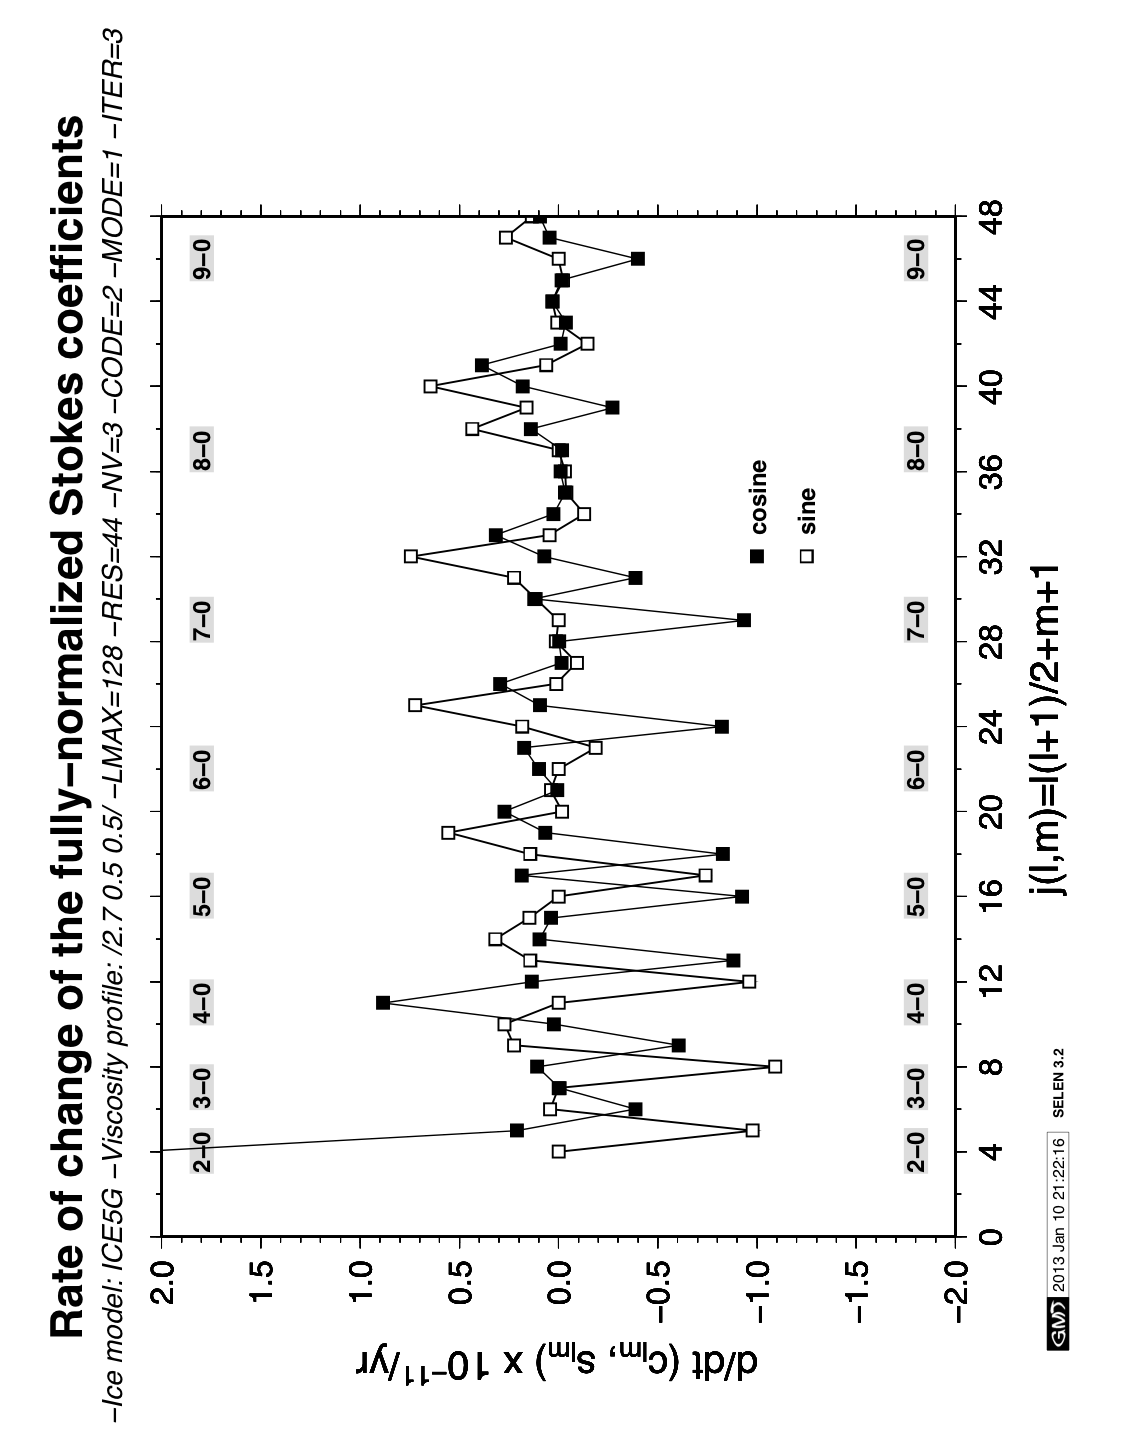
\includegraphics[width=0.78\textwidth, angle=-90]{./Figures/stokes.png}
\caption[Time variation of the Stokes coefficients]{\small{Time--derivatives of the Stokes coefficients of the Earth's gravity field associated with GIA, as a function of the generalized harmonic degree $j=\ell(\ell+1)/2+m+1$ for $2\le \ell\le 9$ and $0\le m \le\ell$, for the \texttt{TEST} run of \selens. Output data for this analysis are stored in folder \texttt{depot-TEST/stokes} after the execution of \selens.}}
\label{fig:stokes}
\end{center}
\end{figure}
\clearpage

\section{Appendices}

\subsection{\selen Fortran units}
%%%%%%%%%%%%%%%%%%%%%%%%%%%%%%%%%%
%
% Table: Fortran units Table: Fortran units Table: Fortran units Table: Fortran units 
%
\begin{table}[!hbp] 
\begin{center}
\caption[{\selen Fortran units}]{\selen Fortran 90 program units.  Source files are stored in the \texttt{src} folder.}
\begin{tabular}{ll}
\\
\hline
Unit name &  Purpose and comments  \\
\hline
\texttt{config.f90} &  \selen setup program  \\[-0.0em]
\texttt{esl.f90} & Equivalent Sea Level \\[-0.0em]
\texttt{geo.f90} & Time variations of geodetic quantities \\[-0.0em]
\texttt{gmaps.f90} & Synthesis of geodetic quantities on global maps \\[-0.0em]
\texttt{harmonics.f90} & Include file with various SH tools and utilities \\[-0.0em]
\texttt{ms.f90} & GMT multi--segment files from ice data \\[-0.0em]
\texttt{of\_dv.f90}& Degree variance of the Ocean Function \\[-0.0em]
\texttt{px.f90}& Pixelization tools (including the Tegmark algorithm)\\[-0.0em]
\texttt{px\_rebuild.f90}& Retrieves pixelization data from an existing pixel table file \\[-0.0em]
\texttt{px\_rec.f90}& Reorganizes the pixelization data \\[-0.0em]
\texttt{rec\_ice.f90}& SH reconstruction of the ice thickness \\[-0.0em]
\texttt{rec\_of.f90}& SH reconstruction of the Ocean Function  \\[-0.0em]
\texttt{rmaps.f90}& Synthesis of geodetic quantities on regional maps \\[-0.0em]
\texttt{rsl.f90}& Relative Sea Level curves \\[-0.0em]
\texttt{rsl\_zones.f90}& Geometry of the Relative Sea Level ``Clark's zones''  \\[-0.0em]
\texttt{rslc.f90}& Relative Sealevel Contour lines for regional analyses \\[-0.0em]
\texttt{sh.f90}& SHs at the grid pixels \\[-0.0em]
\texttt{sh\_of.f90}& SH coefficients for the Ocean Function \\[-0.0em]
\texttt{sh\_rsl.f90}& SHs at the RSL sites \\[-0.0em]
\texttt{sh\_rslc.f90}& SHs for regional analysis and RSL contours  \\[-0.0em]
\texttt{sh\_tgauges.f90}& SHs at the TG sites  \\[-0.0em]
\texttt{shape\_factors.f90}& ``Shape factors'' for the ice elements \\[-0.0em]
\texttt{shice.f90}& SH decomposition of the ice model \\[-0.0em]
\texttt{shtools.f90}& A SHTOOLS interface for the SH analysis \\[-0.0em]
\texttt{sle.f90}& The SLE solver \\[-0.0em]
\texttt{stokes.f90}& Variations of the Stokes coefficients of the gravity field \\[-0.0em]
\texttt{tgauges.f90}& Present--day rate of \sealevel change at the TG sites \\[-0.0em]
\texttt{tb.F90}& The TABOO code \\[-0.0em]
\texttt{wnw.f90} &  Numerical test for the SH orthogonality (`window function")\\
\hline
\label{table:fortran-units}
\end{tabular}
\end{center}
\end{table}
\clearpage 

\subsection{Structure of the \selen output data}
\begin{table}[!hbp] 
\begin{center}
\caption[{\selen output data}]{Structure of the output data in the \texttt{depot} folder of \selens.}
\begin{tabular}{ll}
\\
\hline
{Folder} & Content   \\
\hline
\texttt{ICE5G}                     & Data about the ice model\\[0.0em]
\texttt{~~~ICE5G/esl}                     & ESL \\[0.0em]
\texttt{~~~ICE5G/original}                     & Ice thickness data \\[0.0em]
\texttt{~~~ICE5G/reconstructed}                     & SH reconstruction of ice thickness data\\[0.0em]
\texttt{~~~ICE5G/sh}                     & SH coefficients of the ice model \\[0.0em]
\texttt{Love-Numbers-by-TABOO}            & Love numbers data\\[0.0em]
\texttt{TABOO}   & TABOO input files \\[0.0em]
\texttt{geod}   & Predictions at geodetic sites\\[0.0em]
\texttt{~~~geod/3dmaps}   & Regional maps (in progress) \\[0.0em]
\texttt{~~~geod/sites}   & Geodetic predictions at specific sites \\[0.0em]
\texttt{gmaps}   & Global fingerprints (data and plots) \\[0.0em]
\texttt{log}   & Log files of \selen and TABOO \\[0.0em]
\texttt{of}   & Ocean function data and plots \\[0.0em]
\texttt{~~~of/degree\_variance}   & Ocean function degree variance \\[0.0em]
\texttt{px}   & Various pixelization data and plots \\[0.0em]
\texttt{rmaps}   & Regional fingerprints (data and maps) \\[0.0em]
\texttt{rsl}   & Relative Sea Level (RSL) data folder \\[0.0em]
\texttt{~~~rsl-contours} & RSL contour plot \\[0.0em]
\texttt{~~~rsl-curves} & RSL curves at specific sites \\[0.0em]
\texttt{~~~rsl-misfit}  & Misfit between RSL data and predictions \\[0.0em]
\texttt{~~~rsl-scplot} & Scatterplot of RSL data \\[0.0em]
\texttt{~~~rsl-sites} & Data and plots regarding RSL sites \\[0.0em]
\texttt{~~~rsl-table} & Summary table of RSL data and predictions \\[0.0em]
\texttt{~~~rsl-zones} & RSL zones \\[0.0em]
\texttt{stokes}   &  Stokes coefficients data \\[0.0em]
\texttt{tgauges}   & Tide gauges (TGs) \\[0.0em]
\texttt{~~~tgauges-predictions}  & Predictions at TGs   \\[0.0em]
\texttt{~~~tgauges-scplots}  & TG data scatterplot \\[0.0em]
\texttt{~~~tgauges-sites} & Maps of TG sites\\[0.0em]
\texttt{wnw}   & ``Window test'' for the ocean function \\
\hline
\label{table:folders}
\end{tabular}
\end{center}
\end{table}
\clearpage


\subsection{Ice sheets models in \selen}
%
% Table: Ice models ... Ice models ... Ice models ...
%
\begin{table}[!hbp] 
\begin{center}
\caption[{Ice sheets models}]{Ice sheets models available in the \texttt{ICE-MODELS} folder of \selens. 
For all these models, the details of the chronology and the history of the ice thickness 
are given in the file headers. A rigorous definition of disk-- and cap--shaped 
ice sheets geometries are given by \citet{Spada_etal_2011}. The volume of the ice sheets can be 
assessed running \selen and with option \texttt{221} set to \texttt{'y'}, which will provide the ESL curve 
(an example is given in Fig.~\ref{fig:eustatic} for model ICE--5G.}
\begin{tabular}{lll}
\\
\hline
Ice model file &  Description & Notes \\
\hline
\texttt{alpsc.dat}             &  Alpine ice sheet  & See \citet{Spada_etal_2009} \\
\texttt{~~~~alpsf.dat}         &  a few variants  & ... \\
\texttt{~~~~alpsh.dat}         &  ...  & ... \\
\texttt{~~~~alpst.dat}         &  ...  & ...  \\
\texttt{disk\_off.dat}         &  disk-shaped ice sheet & Instantaneous melting  \\
\texttt{disk\_on.dat}          &  ...                   & Instantaneous freezing \\
\texttt{icap\_off.dat}         &  cap-shaped ice sheet  & Instantaneous melting  \\
\texttt{icap\_on.dat}          &  ...                   & Instantaneous freezing  \\
\texttt{ice1.dat}              &  The ICE--1 ice model  & \citet{Peltier_and_Andrews_1976}\\
\texttt{~~~~ice1\_eup.dat}     &  ICE-1 sub--aggregate  & Europe \\
\texttt{~~~~ice1\_gre.dat}     &  ...                   & Greenland\\
\texttt{~~~~ice1\_nam.dat}     &  ...                   & North America and Canada\\
\texttt{ice3g.dat}             & The ICE--3G ice model  & \citet{Tushingham_and_Peltier_1991}\\
\texttt{~~~~ice3g\_and.dat}    & ICE-3G sub--aggregate   & Andes \\
\texttt{~~~~ice3g\_ant.dat}    & ...                    & Antarctica \\
\texttt{~~~~ice3g\_bal.dat}    & ...                    & Baltic region \\
\texttt{~~~~ice3g\_bar.dat}    & ...                    & Barents Sea  \\
\texttt{~~~~ice3g\_bri.dat}    & ...                    & British Isles  \\
\texttt{~~~~ice3g\_gre.dat}    & ...                    & Greenland\\
\texttt{~~~~ice3g\_ice.dat}    & ...                    & Iceland  \\
\texttt{~~~~ice3g\_nam.dat}    & ...                    & North America and Canada  \\
\texttt{~~~~ice3g\_sib.dat}    & ...                     & Siberia  \\
\texttt{ice5g.dat}            & The ICE--5G ice model   & \citet{Peltier_2004}\\
\texttt{~~~~ice5g\_and.dat}   & ICE-5G sub--aggregate   & Andes \\
\texttt{~~~~ice5g\_ant.dat}   & ...                     & Antarctica \\
\texttt{~~~~ice5g\_fen.dat}   & ...                     & Fennoscandia \\
\texttt{~~~~ice5g\_gre.dat}   & ...                     & Greenland \\
\texttt{~~~~ice5g\_icl.dat}   & ...                    & Iceland \\
\texttt{~~~~ice5g\_lau.dat}   & ...                    & Laurentide \\
\texttt{~~~~ice5g\_nwz.dat}   & ...                    & New Zaeland \\
\hline
\label{table:ice-models}
\end{tabular}
\end{center}
\end{table}
\clearpage


\subsection{Configuration file for the \texttt{TEST} run}\label{sec:sample-config}
For the sake of the reader's convenience, file \texttt{config.dat} for the \texttt{TEST}
run described in Section~\ref{section:test-run} is copied below. This file is 
available from the \selen distribution package. 

{\color{black}{\scriptsize\begin{verbatim}

!!!!!!!!!!!!!!!!!!!!!!!!!!!!!!!!!!!!!!!!!!!!!!!!!!!!!
  This is file "config.dat" for SELEN 2.9 - 
!!!!!!!!!!!!!!!!!!!!!!!!!!!!!!!!!!!!!!!!!!!!!!!!!!!!!

~~~~~~~~~~~~~~~~~~~~~~~~~~~~~~~~~~~~~~~~~~~~~~~~~~~~~~~~~~~~~~~~~~~~~~~~~~~~~~~~~~~~~~~~~~~~~~~~
The user can configure SELEN by the switches below. Any option is to be written within primes 
(e. g., 'option'). A three-digits, left aligned numerical code is provided for each entry (e. 
g., 001). 

In section 1 (settings) the user supplies the spatial resolution, the ice sheets distribution, 
and the Earth model viscoelastic structure. This allows one to solve the Sea Level Equation but 
no graphical output is obtained. 

In section 2 (outputs), a number of optional outputs can be scheduled, including tables and plots 
of numerical results. The required GMT scripts are automatically generated according to the 
options chosen. 

For help, comments, or suggestion, you can contact the authors at the addresses below or consult 
the SELEN web page at http://geodynamics.org/cig/software/selen

Contact: Giorgio Spada <giorgio DOT spada AT gmail DOT com> 
~~~~~~~~~~~~~~~~~~~~~~~~~~~~~~~~~~~~~~~~~~~~~~~~~~~~~~~~~~~~~~~~~~~~~~~~~~~~~~~~~~~~~~~~~~~~~~~~

!!!!!!!!!!!!!!!!!!!!!!!!!!!!!!!!!!!!!!!!!!!!!!!!!!!!!
 This is SECTION (1) of "config.dat": SELEN settings
!!!!!!!!!!!!!!!!!!!!!!!!!!!!!!!!!!!!!!!!!!!!!!!!!!!!!

====> PURGING option ----------------------------------------------------------
110  Purging the wdir before & after execution                      'y'
     [see config.f90 for purged filenames extensions ]

====> SOLUTION of the SLE -----------------------------------------------------
130    Iterations & mode of solution                              '3'    '1' 	    			 	
Modes:  1= Gravitationally self-consistent (GSC)
        2= Elastic GSC / 3="Eustatic" / 4="Woodward" / 5="No Ice" 

====> MAXIMUM HARMONIC DEGREE -------------------------------------------------
140    LMAX     				                       '128'  

====> REFERENCE FRAME ---------------------------------------------------------
145    Includes degree 1 Love numbers (CM/CE frames)             'y'  'CM'   

====> TEGMARK RESOLUTION ------------------------------------------------------
150    R                  				             '44'
151    Prepare a new pixel table (y/n, filename)         'y' 'px-table-r44.dat'

====> RHEOLOGICAL MODEL -------------------------------------------------------
160    Rheological profile info:                         '3' '2' 'vsc_VM2a.dat'  

====> ICE MODEL ---------------------------------------------------------------
170    Ice file name                                               'ice5g.dat'  
171    Prepare a new SH ice file (y/n, filename)       'y'  'ice5g-l128.dat'
172    Ice history time step (kyrs)                       '1.0' 

====> SPHERICAL HARMONICS (SH) FILE AT PIXELS ---------------------------------
180    A new SH file (y/n, filename)                    'y'  'sh-r44-l128.bin'  

====> OCEAN FUNCTION (OF) -----------------------------------------------------
190    A new OF SH decomposition (y/n, filename)         'y'  'of-l128.dat'

====> REPOSITORY LABEL --------------------------------------------------------
195    The depot name  (four characters)                 'TEST' 

!!!!!!!!!!!!!!!!!!!!!!!!!!!!!!!!!!!!!!!!!!!!!!!!!!!!
 This is SECTION (2) of "config.dat: SELEN outputs
!!!!!!!!!!!!!!!!!!!!!!!!!!!!!!!!!!!!!!!!!!!!!!!!!!!!

====> EXECUTION of the GMT SCRIPTS -------------------------------------------- 
200    Execution of GMT scripts during the SELEN run (y/n)     'y'

====> PIXELIZATION & WINDOW ---------------------------------------------------
205    Pixelization maps (y/n)                                  'y'
206    Window function evaluation & plot (y/n)                     'n'

====> OCEAN FUNCTION (OF) -----------------------------------------------------
210    Present-day OF map & reconstruction (y/n)                'y'
215    Plot of OF degree variance (y/n)                            'n'

====> ICE MODEL ---------------------------------------------------------------
220    Maps of original ice sheets  (y/n)                	      'y' 
221    Plot of Equivalent Sea Level (ESL)  (y/n)       		     'y' 
222    Reconstruction & mapping of the ice sheets (y/n)  	    'n'

====> EARTH MODEL SPECTRAL PROPERTIES -----------------------------------------
230    Plot LDCs, relaxation spectrum & residues for normal modes  (y/n)   'y'      

====> RSL PREDICTIONS AT SPECIFIC SITES ---------------------------------------
240    RSL analysis, database & format                'y'  'sealevel.dat'   '0'
241    Plot of RSL sites distribution                         'y' 
242    Site-by-site RSL predictions vs data & plots          'y'  'y'
243    Scatterplot of RSL data & predictions       	    'y' 
244    Misfit between RSL data & predictions               'n'
245    Table with all RSL data & predictions              'y'

====> RSL REGIONS -------------------------------------------------------------
250    Gobal RSL zones  	                           'n'
251    Regional RSL contour lines                           'y'   'rsl-region.dat'

====> SEA LEVEL CHANGE AT TIDE-GAUGE STATIONS --------------------------------- 
260    Tide-gauge (TG) analysis & database                    'y' 'rlr-trends.txt'      
261    Plot of TG stations distribution                      'y'
262    TG data scatterplot   	                            'n' 
263    Table of S, N, and U-dot predictions at TG sites    'y'  

====> GLOBAL PRESENT-DAY RATES ------------------------------------------------
270    Global maps of dot S, U & N               	  'y' 

====> 3D VELOCITY -------------------------------------------------------------
275    -Up, North, East, S, and N rates for sites in file       'n' 'NA_KK.txt'

====> REGIONAL PRESENT-DAY RATES ---------------------------------------------- 
280    Regional maps of dot S, U, & N 	           'n'	     
281      -1 Italy                                   'y'
282      -2 Mediterranean     		             'y'
283      -3 Europe     		                      'y'
284      -4 Fennoscandia   		               'y'
285      -5 Greenland                                   'y'
286      -6 North America  			         'y'
287      -7 Antarctica   		                  'y'

====> STOKES COEFFICIENTS (SC) ------------------------------------------------
290    Rate of change of SC & range of degrees for plot      'y'  '2'  '20'
\end{verbatim} }}


\subsection{Output flow}\label{sec:flow}

The execution of \selen should produce the following output flow on the monitor. The three main
execution steps, described in Section \ref{sec:execution}, are marked on the right side of the page.  The symbol \texttt{[...]} indicates output messages that have been omitted for the sake of clarity.

{\color{Blue}{\scriptsize\begin{verbatim}

- - - - - - - - - - - - - - - - - - - - - - - - - - - - -

     SELEN, a Sea levEL EquatioN solver, Version 2.9

   Send comments, requests of help and suggestions to:
                <giorgio.spada@gmail.com>
                            -
                  Copyright(C) 2008-2013
              Giorgio Spada, Daniele Melini,
            Florence Colleoni & Paolo Stocchi
                          * * *
     This programs comes with  ABSOLUTELY NO WARRANTY
 This is free software and you are welcome to distribute
              it under certain conditions.
    For details, visit  <http://www.gnu.org/licenses/>
                  or edit file COPYING
- - - - - - - - - - - - - - - - - - - - - - - - - - - - -


----------------------------
 >>> 1. Executing SELEN  ...
----------------------------

---> Output data will be stored into directory DEPOTS/depot-TEST

---> Purging the working directory:

---> PX.F90: Hicosahedral pixelization of the sphere       +------------------------------+
[...]                                                      | - STEP 1: Grid, SHs and LDCs |
                                                           +------------------------------+                                                       
---> px.gmt: Separating wet from dry pixels
[...]

---> PX_REC.F90: Merging the wet & dry pixels tables

---> pxmap.gmt: Producing pixelization maps                                                                                
     - wet pixels
     - dry pixels
     - Spherical map of wet and dry pixels

---> SH.F90: Building the spherical harmonics
     - Maximum degree is:          128
     - JMAX is:        8385
     - Resolution is:           44
[...]

---> REC_OF.F90: Reconstructing and mapping the ocean function
[...]

---> Importing ice5g.dat from ICE-MODELS/

---> SHAPE_FACTORS.F90: Computing the shape factors for model: ice5g.dat
[...]

---> SHICE.F90: Computing SH coefficients for the ice model
     - Read        11388   elements from ice5g.dat
[...]

---> MS.F90: Creating multi-segment files for ice sheets maps

---> mapice.gmt: Creating ps images of original ice sheets
[...]

---> TB.F90: Load-deformation coefficients by TABOO (Normal Modes)
     - Calling TABOO
[...]
[...]                                                     +-------------------------------+
[...]                                                     | - STEP 2: Solution of the SLE |
[...]                                                     +-------------------------------+

---> SLE.F90: Solving the Sea Level Equation - SLE - for FIXED coastlines
[...]
     - Starting the recursion                           
     - step  1 of 3
     - step  2 of 3
     - step  3 of 3                                +--------------------------------------+
[...]                                              | - STEP 3: Computation of geophysical |
[...]                                              |           and geodetic variables     |
[...]                                              +--------------------------------------+

---> RSL.F90: Predicting RSL at the sites of database: ./DATA/sealevel.dat
     - Computing the harmonics at the RSL sites
     - Computing sinthetic RSL curves
[...]

---> TGAUGES.F90: Dot-S, U, and N predictions at tide gauges
     - There are        1123 sites in file ./DATA/rlr-trends.txt
     - Rate of sealevel change at site
     -            1 of        1123 REYKJAVIK                     
[...]

---> GMAPS.F90: Global maps of dot S, U and N at present time
[...]
---> STOKES.F90: Present-time rate of change of Stokes coefficients
[...] 
         
------------------------------------                                          +-----------+
 >>> 2. Cleaning up the directory...                                          | - Cleanup |
------------------------------------                                          +-----------+
[...]

- - - - - - - - - - - - - - - - - - - - - - - - - - - - -

     SELEN, a Sea levEL EquatioN solver, Version 2.9

   Send comments, requests of help and suggestions to:
                <giorgio.spada@gmail.com>
                            -
                  Copyright(C) 2008-2013
              Giorgio Spada, Daniele Melini,
            Florence Colleoni & Paolo Stocchi
                          * * *
     This programs comes with  ABSOLUTELY NO WARRANTY
 This is free software and you are welcome to distribute
              it under certain conditions.
    For details, visit  <http://www.gnu.org/licenses/>               +--------------------+
                  or edit file COPYING                               | - End of execution | 
- - - - - - - - - - - - - - - - - - - - - - - - - - - - -            +--------------------+


 >>> Outputs for this run are available in directory: DEPOTS/depot-TEST
\end{verbatim} }} 
\clearpage

\subsection{Conventions for Spherical Harmonics}\label{sec:shs}
In the SLE theory and in program \selens, we 
adopt \textit{complex, $4\pi$--normalized spherical harmonic (SH) functions}: 
\begin{equation}\label{eq:ylm}
{\cal Y}_{\ell m}(\omega) = 
\sqrt{(2\ell +1)\frac{(\ell -m)!}{(\ell +m)!}}
P_{\ell m} (\cos\theta) \textrm{e}^{im\lambda}, 
\end{equation}
where $\omega\equiv (\theta,\lambda)$, $\theta$ is colatitude ($0\le \theta\le \pi$), $\lambda$ is longitude ($0\le \lambda\le 2\pi$), $\ell$ is the harmonic degree ($\ell =0, 1, \ldots$), $m$ is the order 
($m=0, 1, \ldots, \ell$) and $P_{\ell m}(\cos\theta)$ are the associated Legendre polynomials
\begin{equation}\label{eq:plm}
P_{\ell m} (x) =  (-1)^m (1-x^2)^{\frac{m}{2}} \frac{d^m}{dx^m} P_\ell (x), 
\end{equation}
where factor $(-1)^{m}$ is known as the 
Condon--Shortley phase, and 
\begin{equation}
P_\ell(x) = \frac{1}{2^\ell \ell !} \frac{d^\ell}{dx^\ell}(x^2-1)^\ell
\end{equation} 
are the Legendre polynomials. 

SHs with negative order are defined by
\begin{equation}\label{eq:ylm-negative-order}
{\cal Y}_{\ell, -m}(\omega) = {\cal Y}^\ast_{\ell m}(\omega),
\end{equation}
where the asterisk denotes the complex conjugate. By definition (\ref{eq:ylm}), the orthogonality 
condition of the SHs reads 
\begin{equation}
\int_{0}^{2\pi} \int_{0}^\pi {\cal Y}_{\ell m}(\omega) {\cal Y}^*_{\ell' m'}(\omega) d\omega =
4\pi \delta_{\ell \ell'}\delta_{mm'}, 
\end{equation}
where 
\begin{equation}
d\omega \equiv \sin \theta d\theta d\lambda
\end{equation}
and $\delta_{ij}$ is Kronecker delta. In \selens, the SHs are computed numerically 
using routines from the {SHTOOLS} package\footnote{http://www.ipgp.fr/wieczor/SHTOOLS/SHTOOLS.html}.

\subsection{Availability of SELEN}
Program \selen (version 2.9) is hosted by the CIG at the page: \texttt{http://geodynamics.org/cig/software/selen}. \\

\noindent \selen is also available from the web page \textit{http://hpc.rm.ingv.it/selen}, or from the authors. 

\subsection{Related software}
%\marginpar{FINIRE}
\begin{description}
\item[TABOO.] Program TABOO is a post--glacial rebound calculator written in Fortran 90. It is \textit{not} a SLE solver. \selen includes the basic components of TABOO in order to compute the LDCs (see program \texttt{tb.F90}). TABOO, along with its documentation, is available from the Samizdat press\footnote{http://samizdat.mines.edu/taboo/}, 
\item[\textit{s}TABOO.] This is a light version of TABOO, written for absolute beginners. It has been 
written for the students of the PhD course/workshop on Sea Level Rise and Ice Sheets,
held at Center for Ice and Climate, University of Copenhagen (21-25 May, 2012). It
comes with installation instructions and can be obtained by email from GS, 
\item[ALMA.] Program ALMA\footnote{http://www.fis.uniurb.it/spada/ALMA\_minipage.html} \citep{Spada_2008} computes the LDCs for multi--layered Earth models with a generalized Maxwell rheology, adopting a special method of inversion for Laplace transforms~\citep{Spada_and_Boschi_2006}. 
\end{description}

\subsection{Previous reference documents}
Previous versions of \selen and of the theory behind have been described in various papers and documents. 
In these works, the readers can find more details and hints, as well as various references to previous
relevant papers on the subject: 
\begin{itemize}
\item The theory behind the SLE is described in a booklet\footnote{http://samizdat.mines.edu/sle/sle.pdf}
published from the Samizdat Press\footnote{http://www.samizdat.edu} in 2005. This material has been subsequently 
revised and reorganized, and published by \citet{Spada_and_Stocchi_2006}, 
\item the work by \citet{Spada_and_Stocchi_2007} contains a condensed theory of the SLE and illustrates the 
first version of \selens, which in this document is referred to as \selen 1.0, 
\item The current version of \selen (2.9) is presented in the manuscript by \citet{Spada_etal_2012b} (arXiv:1212.5061),
where also some applications are discussed. The present manual is essentially a user--oriented version of this paper.  
\item The Sea Level Equation page on Wikipedia\footnote{http://en.wikipedia.org/wiki/Sea\_level\_equation}
gives a short definition of the SLE.
\end{itemize}

\subsection{SELEN benchmarks}

During the last few years, in the framework of the European COST Action ES0701 ``Improved Constraints on Models of 
Glacial Isostatic Adjustment''\footnote{http://www.cost-es0701.geoenvi.org/}, various benchmark tests on GIA modeling have been performed. 

Until present, the results concerning Post Glacial Rebound modeling have been published in the paper by \cite{Spada_etal_2011}. In
this work, program TABOO (based on the Viscoelastic Normal Modes method of \citeauthor{Peltier_1974}~\citeyear{Peltier_1974}) has been successfully tested against various programs used in the community, often based on completely different techniques. Since \selen computes the LDCs using TABOO, and the LDCs enter the 
Green's functions that appear in the SLE, the \cite{Spada_etal_2011} benchmark
has validated these fundamental components of the program. 

\begin{figure}[!hbp] 
\begin{center}
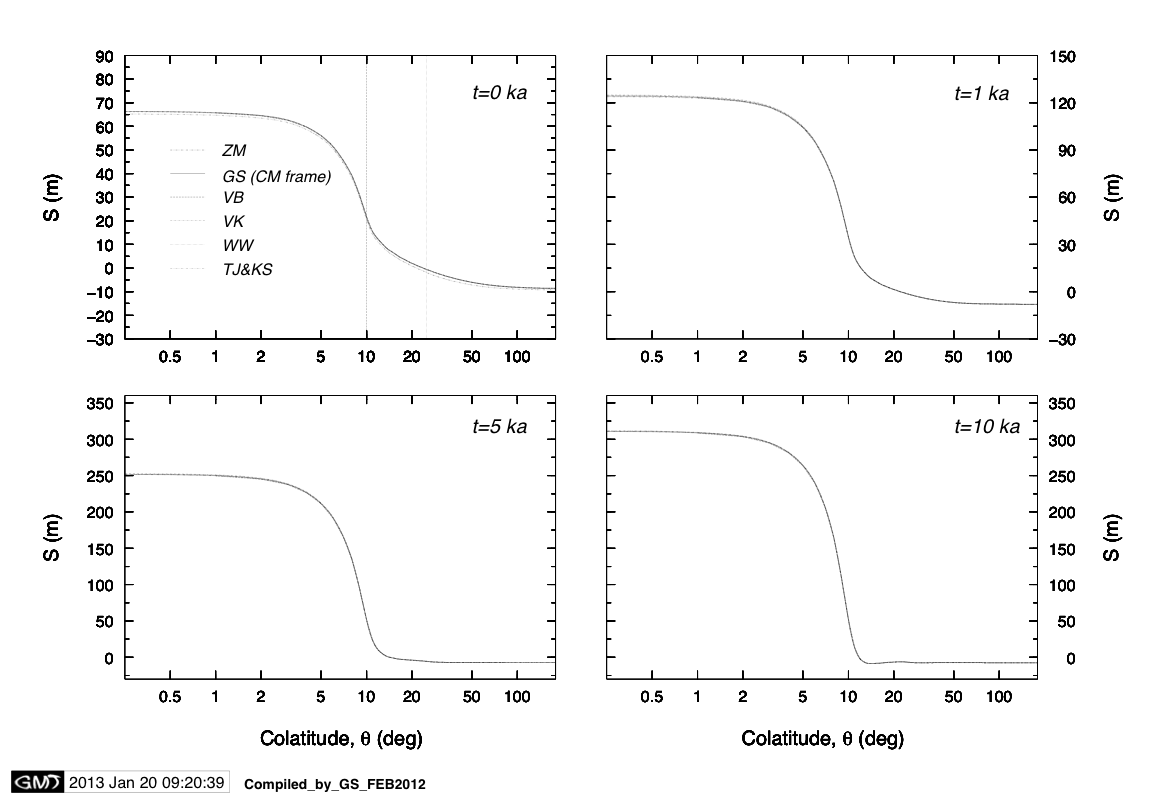
\includegraphics[angle=0,width=0.9\textwidth]{./Figures/s-benchmark.png}
\vspace{0cm}
\caption[SLE benchmark]{\small{Sea level change $S(\omega,t)$ and a function of colatitude, for various times after the load is
imposed $(t=0)$, for the benchmark test described in \cite{Spada_etal_2011}. Vertical segments in the top left frame mark the margin 
of the ice load and the (fixed) continent--ocean boundary.}}
\label{fig:benchmark} 
\end{center} 
\end{figure}

The idea of a SLE benchmark dates back to the mid 1990s, and was first launched by the colleagues Georg Kaufmann and Paul Johnston (the whole story and subsequent developments are reviewed in the Introduction of the \citet{Spada_etal_2011} paper, where some useful links are also given). At the current stage (January 2013), a number of tests computations have been performed in the context of the European COST Action ES0701, and a manuscript is in preparation. 

In Fig.~\ref{fig:benchmark} we show the outcomes of some SLE computations independently performed by Valentina Barletta (VB),
Zdenek Martinec (ZM), Tom James and Karen Simons (TJ\& KS), Volker Klemann (VK), {Wouter van der Wal} (WW)
and myself (GS, based on a suitably designed version of \selens). Here, the SLE is solved assuming an ocean--continents distribution with zonal symmetry wrt the axis $\theta=0^\circ$. The continent, which extends to colatitude $\theta=25^\circ$, is loaded by a ice sheet with 
parabolic profile (i.e., a \textit{cap}, see \citeauthor{Spada_etal_2011}~\citeyear{Spada_etal_2011}) having a thickness of $1500$ m at the
centre and half amplitude $\alpha=10^\circ$, and characterized by a Heaviside time--history (the load is switched on at time $t=0$). The ice and water density are $\rho_w=1000$ kg m$^{-3}$ and $\rho_i =920$ kg m$^{-3}$, respectively. 
Shorelines are not allowed to migrate horizontally and the Earth is not rotating. The rheological model is the same employed in the \citet{Spada_etal_2011} exercise (i.e., the five--layer, incompressible viscoelastic model M3--L70--V01, see their Table 3). \selen has been configured for a ``gravitationally self--consistent'' mode of solutions with three
iterations, with a grid resolution parameter \texttt{R=44}, and a maximum harmonic degree \texttt{LMAX=128}. The SLE is
solved in the CM frame. 

Fig.~\ref{fig:benchmark}, which illustrates the history and the spatial pattern of $S(\omega,t)$, indicates that the various numerical solutions of the SLE are, for this axisymmetric test, substantially in agreement. New tests, which are under way, are
dealing with the
more challenging case of a realistic ocean function and a complex ice sheets distribution. 

\clearpage

\begin{thebibliography}{99}

\bibitem[Amdahl(1967)]{Amdahl_1967}
Amdahl G (1967) 
Validity of the single processor approach to achieving large--scale computing capabilities.
AFIPS Conference Proceedings, 30:483--485, AFIPS Press.

\bibitem[Clark {et al.}(1978)]{Clark_etal_1978}
Clark JA, Farrell WE, Peltier WR (1978) 
Global changes in postglacial sea level: a numerical calculation.  
Quat. Res. 9:265--287. 

%\bibitem[Dahlen(1976)]{Dahlen_1976}
%Dahlen FA (1976)
%The passive influence of the oceans upon the rotation of the Earth. 
%Geophys. J. R. Astron. Soc. 46:363--406.

\bibitem[Farrell and Clark(1976)]{Farrell_and_Clark_1976}
Farrell WE, Clark JA (1976) 
On postglacial sea--level. 
\gjras 46:647--667. 

\bibitem[Milne(1998)]{Milne_1998}
Milne GA (1998) 
Refining models of the glacial isostatic adjustment process.
Ph. D. Dissertation, University of Toronto, Toronto, CA, (126 pp). 

%\bibitem[Milne and Mitrovica(1998)]{Milne_and_Mitrovica_1998}
%Milne GA, Mitrovica JX (1998) 
%Postglacial sea--level change on a rotating Earth. 
%\gji 133(1):1--19, doi:10.1046/j.1365-246X.1998.1331455.x 

%\bibitem[Mitrovica and Milne(2003)]{Mitrovica_and_Milne_2003}
%Mitrovica JX, Milne GA (2003) 
%On post--glacial sea level: I. General theory. 
%\gji 154(2):253--267, doi:10.1046/j.1365-246X.2003.01942.x 

%\bibitem[Mitrovica {et al.}(2003)]{Mitrovica_etal_2003}
%Kendall RA, Mitrovica JX, Milne GA (2003) 
%On post--glacial sea level: II. Numerical formulation and
%comparative results on spherically symmetric models
%\gji 161(2):679--706, doi: 10.1111/j.1365-246X.2005.02553.x 

\bibitem[Mitrovica and Peltier(1991)]{Mitrovica_and_Peltier_1991}
Mitrovica JX, Peltier WR (1991) 
On post--glacial geoid subsidence over the equatorial ocean. 
\jgr 96:20,053--20,071.

\bibitem[Mitrovica {et al.}(1994)]{Mitrovica_etal_1994}
Mitrovica JX, Davis JL, Shapiro II (1994) 
A spectral formalism for computing three--dimensional deformations due to surface loads. 
\jgr 99:7057--7073.

\bibitem[OpenMP(2005)]{Openmp_2005}
OpenMP (2005) 
OpenMP Application Program Interface, Version 2.5. OpenMP Architecture Review Board, 
http://www.openmp.org/mpdocuments/spec25.pdf (last accessed 2011). 

\bibitem[Peltier(1974)]{Peltier_1974}
Peltier WR (1974) 
The impulse response of a Maxwell earth. 
Rev. Geophys. Space Phys. 12:649--669.  

\bibitem[Peltier and Andrews(1976)]{Peltier_and_Andrews_1976}
Peltier WR, Andrews TS (1976)
Glacial--isostatic adjustment, I, The forward problem, 
Geophys. J. R. Astr. Soc. 46:605-646. 

%\bibitem[Peltier \textit{et al.}(1978)]{Peltier_etal_1978}
%Peltier, W. R., Farrell, W. E., Clark, J. A., 1978.  
%Glacial isostasy and relative sea level: a global finite element model. 
%Tectonophys. 50, 81--110. 

\bibitem[Peltier(2004)]{Peltier_2004}
Peltier WR (2004)
Global glacial isostasy and the surface of the Ice--Age Earth: the ICE--5G(VM2) model and GRACE. 
Annu. Rev. Earth Pl. Sc. 32:111--149.  

\bibitem[Spada(2003a)]{Spada-2003a}
Spada G (2003) 
The theory behind TABOO. 
Samizdat Press, Golden, Colorado (http://samizdat.mines.edu/taboo/teoria.pdf) 

\bibitem[Spada(2003b)]{Spada-2003b}
Spada G (2003) 
TABOO user guide 
Samizdat Press, Golden, Colorado (http://samizdat.mines.edu/taboo/user\_guide.pdf)
  
\bibitem[Spada~{et al.}(2004)]{tabooeos}
Spada G, Antonioli A, Boschi L, Cianetti S, Galvani G, Giunchi C, Perniola B, 
  Piana Agostinetti N, Piersanti A, Stocchi P (2004) 
  Modeling Earth's post--glacial rebound.
  \eos  85:62--64.  

\bibitem[Spada and Boschi(2006)]{Spada_and_Boschi_2006}
Spada G, Boschi L (2006) 
Using the Post--Widder formula to compute the Earth's viscoelastic Love numbers. 
Geophys. J. Int., 166(1):309--321. doi: 10.1111/j.1365- 246X.2006.02995.x

\bibitem[Spada and Stocchi(2006)]{Spada_and_Stocchi_2006}    
  Spada G, Stocchi P (2006) 
  The Sea Level Equation, Theory and Numerical Examples. 
  Aracne, Roma.
  
\bibitem[Spada and Stocchi(2007)]{Spada_and_Stocchi_2007}   
  Spada G, Stocchi P (2007) 
  \selens: a Fortran 90 program for solving the ``Sea Level Equation'', 
  Comput. and Geosci. 33(4):538--562. doi: 10.1016/j.cageo.2006.08.006

\bibitem[Spada(2008)]{Spada_2008}
Spada G (2008) 
ALMA, a Fortran program for computing the visco--elastic Love numbers of a spherically symmetric planet. 
Comput. and Geosci. 4(6):667-687. doi: 0.1016/j.cageo.2007.12.001.

\bibitem[Spada~{et al.}(2009)]{Spada_etal_2009}
Spada G, Stocchi P, Colleoni F (2009)
Glacio--isostatic Adjustment in the Po Plain and in the Northern Adriatic Region.
Pure appl. geophys. 166:1303--1318. doi: 10.1007/s00024-004-0498-9

\bibitem[Spada~{et al.}(2011)]{Spada_etal_2011}
Spada G, Barletta VR, Klemann V, Riva REM, Martinec Z, Gasperini P, 
Lund B, Wolf D, Vermeersen LLA, King M (2011) A 
benchmark study for glacial--isostatic adjustment codes. \gji 185:106--132. 
doi:10.1111/j.1365-246X.2011.04952.x

\bibitem[Spada and Galassi(2012)]{Spada_and_Galassi_2012}
Spada G, Galassi G (2012)
New estimates of secular sea level rise from tide gauge data and GIA modelling.
\gji 191(3):1067--1094, doi:10.1111/j.1365-246X.2012.05663.x

\bibitem[Spada~{et al.}(2012a)]{Spada_etal_2012a}
Spada G, Ruggieri G, Sorensen LS, Nielsen K, Melini D., Colleoni F (2012a) 
Greenland uplift and regional sea level changes from ICESat observations and GIA modelling.
\gji {189}:1457--1474. doi: 10.1111/j.1365-246X.2012.05443.x

\bibitem[Spada~{et al.}(2012b)]{Spada_etal_2012b}
Spada G, Melini D, Galassi G, Colleoni F (2012b) 
Modeling sea level changes and geodetic variations by glacial isostasy: the improved SELEN code  
(http://arxiv.org/abs/1212.5061). 

\bibitem[Stocchi and Spada(2007)]{Stocchi_and_Spada_2007}
Stocchi P, Spada G (2007)    
Glacio and hydro--isostasy in the Mediterranean Sea: Clark's zones and role of remote ice sheets.
Ann. Geophys. 50(6):741--761. 

\bibitem[Tegmark(1996)]{Tegmark_1996}
Tegmark M (1996)  
An icosahedron--based method for pixelizing the celestial sphere.  
ApJ Letters 470:L81--L84 (http://arxiv.org/pdf/astro-ph/9610094v1.pdf). 

\bibitem[Tushingham and Peltier(1991)]{Tushingham_and_Peltier_1991}
Tushingham AM, Peltier  WR (1991) 
ICE--3G - A new global model of late Pleistocene deglaciation based upon geophysical predictions 
of Post--Glacial relative sea level change.
\jgr 96:4497--4523. 

\bibitem[Tushingham and Peltier(1992)]{Tushingham_and_Peltier_1992}
Tushingham AM, Peltier WR (1992) 
Validation of the ICE--3G model of W\"urm--Winsconsin deglaciation using a global data base of relative sealevel histories. 
\jgr 97:3285--3304. 

\bibitem[Tushingham and Peltier(1993)]{Tushingham_and_Peltier_1993}
Tushingham AM, Peltier WR (1993)   
Relative Sea Level Database. IGPB PAGES/World Data Center--A
for Paleoclimatology Data Contribution Series \# 93--106. 
NOAA/NGDC Paleoclimatology Program, Boulder, USA. 

\bibitem[Wessel and Smith(1998)]{Wessel_and_Smith_1998}
Wessel P, Smith WHF (1998)   
New, improved version of generic mapping tools released. 
\eos 79:579.

\bibitem[Woodward(1888)]{Woodward_1888}
Woodward RS (1888) 
On the form and position of mean sea level.  
United States Geol. Survey Bull. 48:87--170. 

%\bibitem[Wu and Peltier(1983)]{Wu_and_Peltier_1983} 
%Wu, P., Peltier, W. R., 1983. 
%Glacial isostatic adjustment and the free--air gravity anomaly as a constraint on deep 
%mantle viscosity. 
%Geophys. J. R. Astron. Soc. 74, 377--449. 

\end{thebibliography}

\clearpage

\begin{figure}[h]
\begin{center}
\vspace{6cm}

\includegraphics[angle=0,width=1\textwidth]{./Figures/logo_SELEN29.png}
\vspace{0cm}
%\caption[The \selen logo]{\small{The \selen logo is an artwork by Florence Colleoni (2009).}}
%\label{fig:logo} 
\end{center} 
\end{figure}


\end{document}
